% Initial version by Darian Muresan, Ph.D.
% dmuresan@stevens.edu
% Edit and adjust as needed.
\documentclass[12pt]{cornell}
\usepackage[usenames, dvipsnames]{xcolor}

% add index support
%\usepackage{imakeidx}
\usepackage{makeidx}
%\makeindex

% graphing programs
\usepackage{color}
\usepackage{psfrag}
\usepackage{verbatim}
\usepackage{fancyhdr}
%\usepackage{titlesec}
\usepackage{fancyvrb} 
% hyperlink programs
%\usepackage{url}

\usepackage{minted}        % enables the minted environment
\usemintedstyle{friendly}  % optional style
% better typewriter font + proper encodings
\usepackage[T1]{fontenc}
\usepackage{lmodern}        % or \usepackage{newtxtext,newtxmath} if your template uses Times
\usepackage{inconsolata}    % nicer \texttt, helps avoid OMS font-shape warnings

% URLs/paths that can break across lines
\usepackage{url}            % \url and \path
\usepackage{hyperref}

% minted (remember: enable Shell escape in Overleaf settings)
\usepackage{minted}
\usemintedstyle{friendly}
\setminted{breaklines, breakanywhere, fontsize=\small}


% Does not work with LaTeX=>PDF
\usepackage[pdfmark, 
breaklinks=true, 
colorlinks=true,
citecolor=blue,
linkcolor=blue,
menucolor=black,
pagecolor=black,
urlcolor=blue
]{hyperref} % links in pdf

%\usepackage[colorlinks]{hyperref} % links in dvi
\usepackage{listings}
\usepackage{amsfonts} 
\usepackage{amssymb} 
%\usepackage{tabto}

\usepackage{tabularx,colortbl}
\usepackage[chapter]{algorithm} 
\usepackage{algorithmic} 
\usepackage{blindtext}

\definecolor{DarkGreen}{rgb}{0,0.6,0}
\definecolor{mygreen}{rgb}{0,0.6,0}
\definecolor{mygray}{rgb}{0.5,0.5,0.5}
\definecolor{mymauve}{rgb}{0.58,0,0.82}

\usepackage{tocloft}
\usepackage{amsmath}
\usepackage{tcolorbox}
\usepackage{enumitem}
\usepackage{longtable}
%\usepackage{textcomp}
\usepackage{txfonts}
\usepackage{pstool}

%part for \part titles
%chap for \chapter titles
%sec for \section titles
%subsec for \subsection titles
%subsubsec for \subsubsection titles
%para for \paragraph titles
%subpara for \subparagraph titles
%fig for figure \caption titles
%subfig for subfigure \caption titles
%tab for table \caption titles
%subtab for subtable \caption titles


% update chapter number spacing
\setlength{\cftchapnumwidth}{2em}
\setlength{\cftsecnumwidth}{2.5em}
\setlength{\cftsubsecnumwidth}{3.5em}
\setlength{\cftsubsubsecnumwidth}{4.5em}

\addtolength{\cftsecindent}{0.5em}
\addtolength{\cftsubsecindent}{0.5em}
\addtolength{\cftsubsubsecindent}{0.5em}

%\titlespacing*{\chapter}{0pt}{-50pt}{20pt}
%\titleformat{\chapter}[display]{\normalfont\huge\bfseries}{\chaptertitlename\ 
%\thechapter}{20pt}{\Huge}
%\pagestyle{fancy}
%\pagestyle{cornell}
%
%\rhead{F054-021-0172}
%\chead{Nonlinear Enhancement of Visual Target Detection (AF05-T021)}
%\lhead{GSTI}
%\lfoot{\scriptsize Use or disclosure of data on this page is subject
%to the restriction on the title page of this proposal.}
%\cfoot{}
%\rfoot{\thepage}

\newfont{\Bp}{msbm10}
\newfont{\BpBig}{msbm10 scaled\magstep2}
\newfont{\Sc}{eusm10}
\newfont{\ScBig}{eusm10 scaled\magstep3}
\newfont{\Fr}{eufm10}
\newfont{\FrBig}{eufm10 scaled\magstep1}

% some commands:
\newcommand{\dxi}{{\tt m\_xDeltaInput}}
\newcommand{\dyi}{{\tt m\_yDeltaInput}}
\newcommand{\dci}{{\tt m\_cDeltaInput}}
\newcommand{\dxo}{{\tt m\_xDeltaOutput}}
\newcommand{\dyo}{{\tt m\_yDeltaOutput}}
\newcommand{\dco}{{\tt m\_cDeltaOutput}}
\newcommand{\ttf}[1]{{\tt #1}}
\newcommand{\tbl}[2]{{\begin{tabular}{c} #1 \\ #2 \end{tabular}}}

\newcommand{\urltwo}[2]{\mbox{\href{#1}{\tt #2}}}
\newcommand{\qnorm}[1]{\|#1\|_{\bQ}}
\newcommand{\qdot}[2]{\lrb #1, #2 \rrb_{\bQ}}
\newcommand{\kdot}[2]{\lrb #1, #2 \rrb_{\bf k}}
\newcommand{\tdot}[2]{\lrb #1, #2 \rrb}
\newcommand{\mydiff}[2]{\lrb #1 - #2 \rrb}
\newcommand{\lena}{\textit{lena}}
\newcommand{\barb}{\textit{barbara}}
\newcommand{\boat}{\textit{boat}}
\newcommand{\leaves}{\textit{leaves}}
\newcommand{\rings}{\textit{rings}}
\newcommand{\treg}{\textit{train region}}
\newcommand{\dreg}{\textit{denoise region}}
\newcommand{\oreg}{\textit{overlap region}}
\newcommand{\sil}{\sigma_l^2}
\newcommand{\sn}{\sigma^2}
\newcommand{\bn}{{\mbox{\bf \FrBig N}}}
\newcommand{\n}{\mbox{\Fr N}}
%\newcommand{\bn}{\bf N}
%\newcommand{\n}{N}
\newcommand{\bY}{\textbf{Y}}
\newcommand{\bX}{\textbf{X}}
\newcommand{\bb}{\textbf{b}}
\newcommand{\bu}{\textbf{u}}
\newcommand{\bv}{\textbf{v}}
\newcommand{\by}{\textbf{y}}
\newcommand{\bx}{\textbf{x}}
\newcommand{\be}{\textbf{e}}
\newcommand{\bz}{\textbf{z}}
\newcommand{\bs}{\textbf{s}}
\newcommand{\bw}{\textbf{w}}
\newcommand{\bQ}{\textbf{Q}}
\newcommand{\bphi}{\textbf{$\phi$}}
\newcommand{\lsb}{\left[}
\newcommand{\rsb}{\right]}
\newcommand{\lrb}{\left(}
\newcommand{\rrb}{\right)}
\newcommand{\lcb}{\left\{}
\newcommand{\rcb}{\right\}}
\newcommand{\R}{\mbox{\BpBig R}}
\newcommand{\F}{{\cal F}}
\newcommand{\Fk}{\mbox{\Sc F}}
\newcommand{\bQF}{\textbf{Q}_{\mbox{\Sc F}}}
\newcommand{\N}{{\cal N}}
\newcommand{\xlz}{X_l(z)}
\newcommand{\xhz}{X_h(z)}
\newcommand{\xz}{X(z)}
\newcommand{\pr}{ perfect reconstruction }
\newcommand{\smb}{Smith-Barnwell }
\newcommand{\xw}{X(e^{j\omega})}
\newcommand{\xmw}{X(-e^{j\omega})}
\newcommand{\dw}{D(e^{j\omega})}
\newcommand{\dmw}{D(-e^{j\omega})}
\newcommand{\ew}{E(e^{j\omega})}
\newcommand{\emw}{E(-e^{j\omega})}
\newcommand{\fw}{F_0(e^{j\omega})}
\newcommand{\fmw}{F_0(-e^{j\omega})}
\newcommand{\hoz}{H_1(z)}
\newcommand{\hzz}{H_0(z)}
\newcommand{\goz}{G_1(z)}
\newcommand{\gzz}{G_0(z)}
\newcommand{\hzw}{H_{0}(e^{j\omega})}
\newcommand{\hzmw}{H_{0}(-e^{j\omega})}
\newcommand{\hzcw}{H_{0}(e^{-j\omega})}
\newcommand{\how}{H_1(e^{j\omega})}
\newcommand{\homw}{H_1(-e^{j\omega})}
\newcommand{\gzw}{G_0(e^{j\omega})}
\newcommand{\gzmw}{G_0(-e^{j\omega})}
\newcommand{\gow}{G_1(e^{j\omega})}
\newcommand{\gomw}{G_1(-e^{j\omega})}
\newcommand{\wl}{e^{-jwL}}
\newcommand{\aqua}{\textit{AQua with OR }}
\newtheorem{theorem}{Theorem}
\newtheorem{lemma}{Lemma}
\newtheorem{corollary}{Corollary}
\newtheorem{claim}{Claim}
\newtheorem{definition}{Definition}
\newenvironment{proof}{\noindent{\em Proof.}}{\ \hfill Q.E.D.}
%\newtheorem{moduleCount}{L}
\newcommand*{\labelfile}[1]{%
  \label{file:#1}%
}

% Use this to label requirements, use cases, user stories, etc.
% This is where we can add different spellings for different types of 
% requirements, use cases, user stories, etc.
% \newtheorem{requirementKind}{Requirement Spelling}
\newtheorem{reqkFunctional}{Functional Requirement}
\newtheorem{reqkQuality}{Quality Requirement}
\newtheorem{reqkConstraint}{Constraint Requirement}
\newtheorem{reqkInterface}{Interface Requirement}
\newtheorem{reqkBusiness}{Business Requirement}
% Use cases
\newtheorem{useCase}{Use Case}
% User story
\newtheorem{userStory}{User Story}

% command for adding a version to the document
\newcommand{\VERSION}{Version 0.0.0}

% Family -- enter the name of the family that it belongs to: Chapter, Figure, Table, etc.
% Name -- name of the family member: file name, table name, etc.
\newcommand{\FamilyName}[2]{\hyperref[#1::#2]{#2}\index{#2}\xspace}
% Family -- same as above
% Name -- same as above
% Reference -- shorthand for the 'Name'.  It will show as Reference_NameID
% Kind -- underscore(_), space, or dash (-)
\newcommand{\FamilyNameReferenceKind}[4]{\hyperref[#1::#2]{$#3#4{\ref*{#1::#2}}$}}
% newcommand{Family,Label}
\newcommand{\FamilyLabel}[2]{\label{#1::#2}}


% for use cases
\newcommand{\UseCaseLabel}[1]{\FamilyLabel{UseCase}{#1}}
\newcommand{\UseCaseName}[1]{\FamilyName{UseCase}{#1}}
\newcommand{\UseCaseReference}[1]{\FamilyNameReferenceKind{UseCase}{#1}{UC}{_}}
% UseCase name with stacked reference
\newcommand{\UseCaseNameWSReference}[1]{\begin{tabular}{c}\UseCaseName{#1} \\ (\UseCaseReference{#1}) \end{tabular}}
% UseCase name with inline reference
\newcommand{\UseCaseNameWIReference}[1]{\UseCaseName{#1} (\UseCaseReference{#1})}

% for chapters
\newcommand{\ChapterName}[1]{\FamilyName{Chapter}{#1}}
\newcommand{\ChapterLabel}[1]{\FamilyLabel{Chapter}{#1}}
\newcommand{\ChapterReference}[1]{\FamilyNameReferenceKind{Chapter}{#1}{Chapter}{\mbox{ }}}
% Chapter name with inline (WI) reference 
\newcommand{\ChapterNameWIReference}[1]{\ChapterName{#1} (\ChapterReference{#1})}

% for figures
\newcommand{\FigureName}[1]{\FamilyName{Figure}{#1}}
\newcommand{\FigureLabel}[1]{\FamilyLabel{Figure}{#1}}
\newcommand{\FigureReference}[1]{\FamilyNameReferenceKind{Figure}{#1}{Figure}{\mbox{ }}}
% Figure name with stacked (WS) reference
\newcommand{\FigureNameWSReference}[1]{\begin{tabular}{c}\FigureName{#1} \\ (\FigureReference{#1}) \end{tabular}}
% Figure name with inline (WI) reference 
\newcommand{\FigureNameWIReference}[1]{\FigureName{#1} (\FigureReference{#1})}

% for tables
\newcommand{\TableName}[1]{\FamilyName{Table}{#1}}
\newcommand{\TableLabel}[1]{\FamilyLabel{Table}{#1}}
\newcommand{\TableReference}[1]{\FamilyNameReferenceKind{Table}{#1}{Table}{\mbox{ }}}

% for requirements
% RequirementLabel[Kind][Label]
\newcommand{\RequirementLabel}[2]{\FamilyLabel{#1}{#2}}
\newcommand{\RequirementName}[2]{\FamilyName{#1}{#2}}
\newcommand{\RequirementReference}[2]{\FamilyNameReferenceKind{#1}{#2}{#1}{_}}
% Requirements name with stacked (WS) reference
\newcommand{\RequirementNameWSReference}[2]{\begin{tabular}{c}\RequirementName{#1}{#2} \\ (\RequirementReference{#1}{#2}) \end{tabular}}
% Requirements name with inline (WI) reference 
\newcommand{\RequirementNameWIReference}[2]{\RequirementName{#1}{#1} (\RequirementReference{#1}{#2})}

% for requirements
% RequirementLabel[Kind][Label]
\newcommand{\UserStoryLabel}[2]{\FamilyLabel{#1}{#2}}
\newcommand{\UserStoryName}[2]{\FamilyName{#1}{#2}}
\newcommand{\UserStoryReference}[2]{\FamilyNameReferenceKind{#1}{#2}{R}{_}}
% Requirements name with stacked (WS) reference
\newcommand{\UserStoryNameWSReference}[2]{\begin{tabular}{c}\RequirementName{#1}{#2} \\ (\RequirementReference{#1}{#2}) \end{tabular}}
% Requirements name with inline (WI) reference 
\newcommand{\UserStoryNameWIReference}[2]{\RequirementName{#1}{#1} (\RequirementReference{#1}{#2})}



\lstset{ %
  backgroundcolor=\color{white},   % choose the background color; you must add \usepackage{color} or \usepackage{xcolor}
  basicstyle=\footnotesize,        % the size of the fonts that are used for the code
  breakatwhitespace=false,         % sets if automatic breaks should only happen at whitespace
  breaklines=true,                 % sets automatic line breaking
  captionpos=b,                    % sets the caption-position to bottom
  commentstyle=\color{DarkGreen},    % comment style
  deletekeywords={...},            % if you want to delete keywords from the given language
  escapeinside={\%*}{*)},          % if you want to add LaTeX within your code
  extendedchars=true,              % lets you use non-ASCII characters; for 8-bits encodings only, does not work with UTF-8
  %frame=single,                   % adds a frame around the code
  keepspaces=true,                 % keeps spaces in text, useful for keeping indentation of code (possibly needs columns=flexible)
  keywordstyle=\color{blue},       % keyword style
  language=C++,                    % the language of the code
  morekeywords={*,...},            % if you want to add more keywords to the set
  numbers=left,                    % where to put the line-numbers; possible values are (none, left, right)
  numbersep=5pt,                   % how far the line-numbers are from the code
  numberstyle=\tiny\color{mygray}, % the style that is used for the line-numbers
  rulecolor=\color{black},         % if not set, the frame-color may be changed on line-breaks within not-black text (e.g. comments (green here))
  showspaces=false,                % show spaces everywhere adding particular underscores; it overrides 'showstringspaces'
  showstringspaces=false,          % underline spaces within strings only
  showtabs=false,                  % show tabs within strings adding particular underscores
  stepnumber=1,                    % the step between two line-numbers. If it's 1, each line will be numbered
  stringstyle=\color{mymauve}     % string literal style
  %tabsize=2,                      % sets default tabsize to 2 spaces
  %caption=\lstname                % show the filename of files included with \lstinputlisting; also try caption instead of title
}


% Uncomment draftcopy to get the word DRAFT boldly across the first page
%   By the way, xdvi won't show it but it will come out when you print
%\usepackage[light,all]{draftcopy}		% DRAFT on first page
%\draftcopySetGrey{.97}
%\draftcopyName{Confidential}{150}
%\draftcopFirstPage{1}

% Uncomment drafthead to get the date and DRAFT in the header of pages
% that are normallly numbered on the top, pages 2-n of each chapter for example
% This doesn't work with centered page numbers: \pagestyle{cornellc}
%\usepackage{drafthead}

% glossaries to organize the document glossary
%\usepackage[toc,chapter,numberedchapter = autolabel]{glossaries}
\usepackage{glossaries}

% glossary creation
\newglossaryentry{must}
{	name={MustHave},
	description={This defines the first highest priority requirement.
	All of the tasks, requirements, or anything that is marked this way are
	build in the current version}
}

\newglossaryentry{should}
{	name={ShouldHave},
	description={This defines the second highest priority requirement. The system should implement 
	all of the tasks, requirements, or anything that is marked this way, but if 
	resources are limited, it can be left out of the current version.
	Build in next version}
}

\newglossaryentry{could}
{	name={CouldHave},
	description={This defines the third highest priority requirement.The system could implement 
	all of the tasks, requirements, or anything that is marked this way, but if 
	resources are limited, it can be left out of the current and next version.
	Build in two versions from now}
}

\newglossaryentry{would}
{	name={WouldHave},
	description={This defines the lowest priority requirement.  The system would like to implement 
all of the tasks, requirements, or anything that is marked this way, but only
if resources are available. It can be left out of all future versions}
}

%\makeglossaries
\makenoidxglossaries
\makeindex

% Including selective chapters:
% use this to selectively process chapters, etc.  Put a % in front of
% the sections that you don't want done this time.  Includes are
% used instead of \input so that LaTeX will keep track of chapters and
% pages without processing everything.  Don't let any spaces creep in
% around the words or it will not work!

\includeonly{
prologue,
% itIntroduction,
itHosts,
itPasswords,
itLinuxCommands,
itAppendix, 
itProjectProposal,
itAWSDeployment,
itLaTeXDocker,
itBugzilla,
itOverleaf, 
itDomainNames,
itGitHubActions
}


\begin{document}

\pagenumbering{roman}
\singlespacing
% File: prologue.tex
% Thesis prologue:  Title page, acknowledgements, table of contents,
% list of figures, and list of tables.
%
% this file is to be \include'd after the \begin{document}

% Cornell-style title page
\begin{titlepage}
        \title{SSW 590 Group 11}
        \author{Charles Villa, Justin Phan, Benedict Martinez, Jacky Lei \\ cvilla@stevens.edu, jphan1@stevens.edu, bmartin5@stevens.edu, jlei7@stevens.edu }
        \conferraldate{}{\today} \maketitle
\end{titlepage}

% Copyright page
%\begin{copyrightpage}
\makecopyright
%\end{copyrightpage}

% Abstract: the abstract body is pulled from the file abstract.tex;
%  the title is pulled from the \title command in the titlepage section
\begin{abstract}
        %\makeabstitle
        \input abstract      % puts the abstract file here
\end{abstract}

% Biographical information pulled from file bio.tex
%\begin{biosketch} \input bio \end{biosketch}

% Dedication (optional):  pulls information from file dedication.tex
%\begin{dedication} 
%\input dedicate 
%\end{dedication}

% Acknowledgements:  pulls information from file acknow
%\begin{acknowledgements} \input acknow \end{acknowledgements}

% Table of contents
\contentspage

% If you have no tables or figures put a % in front of the list page line
% List of tables
\tablelistpage

% List of figures
\figurelistpage

\setcounter{page}{1}        % set page counter
\pagenumbering{arabic}      % set page number style
\pagestyle{fancy}         % top right page numbers
%\pagestyle{cornell}
%\pagestyle{cornellc}       % centered page numbers, disables drafthead

\renewcommand{\chaptermark}[1]{\markboth{#1}{}}
\renewcommand{\sectionmark}[1]{\markright{#1}{}}

\fancyhead{} % clear all fields

\lhead{Chapter \thechapter}
%\lhead{\thechapter}
\chead{\leftmark}
\rhead{\thepage}


\lfoot{Chapter \thechapter}
\cfoot{\copyright Stevens -- \today \mbox{} -- Do Not Distribute!}
\rfoot{\thepage}

\renewcommand{\headrulewidth}{0.4pt}
\renewcommand{\footrulewidth}{0.4pt}

%\rhead{F054-021-0172}
%\chead{Nonlinear Enhancement of Visual Target Detection (AF05-T021)}
%\lhead{GSTI}
%\lfoot{\scriptsize Use or disclosure of data on this page is subject
%to the restriction on the title page of this proposal.}
%\cfoot{}
%\rfoot{\thepage}


\singlespacing
% \chapter{Introduction \\
\small{\textit{-- Author Name}}
\index{introduction} 
\index{Chapter!Introduction}
\label{Chapter::Introduction}}

 
All projects should have a small introduction.  Here we provide some
example LaTeX commands.  The first example, which is commented out in LaTeX,
is how to introduce an EPS file as an image into the document.

Here is a sample citation \cite{GM1998}.

\begin{verbatim}
\begin{figure}
\psfrag{a }{\Large stvDataObject}
\psfrag{b }{\large Object 1}
\psfrag{c }{\large Object 2}
\psfrag{d }{\large Object N}
\psfrag{e }{\large $Count:N$}
\psfrag{f }
{\hspace{-0.2in}\large \begin{tabular}{c} Sample \\ Table \end{tabular}}
\centering
\scalebox{1}{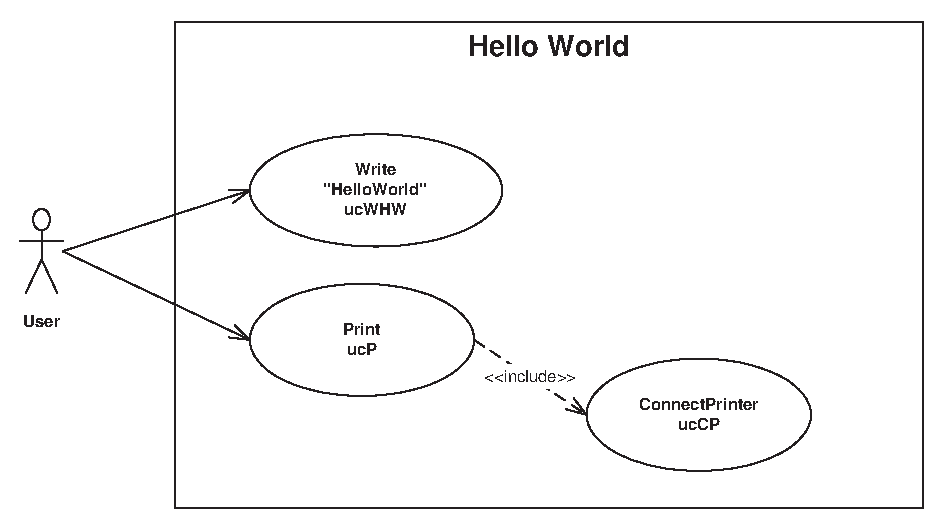
\includegraphics{eps/dsnHelloWorld.eps}}
\caption{\label{Figure::dsnHelloWolrd} Sample EPS image.}
\end{figure}
\end{verbatim}

\noindent
If using Overleaf, then you include a PNG or a JPG file as shown next:

\begin{verbatim}
\begin{figure}
\centering
\scalebox{0.8}{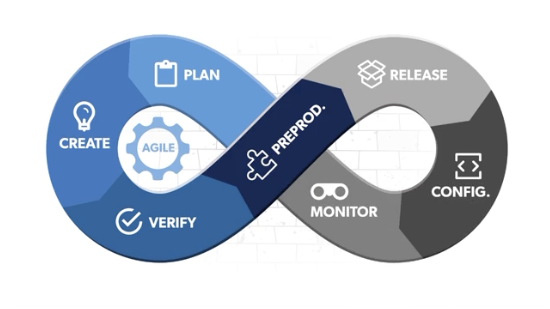
\includegraphics{png/stvAgileProcess.png}}
\caption{\label{Figure::stvAgile} PNG Image included.}
\end{figure}
\end{verbatim}

%\begin{figure}
%\centering
%\scalebox{0.8}{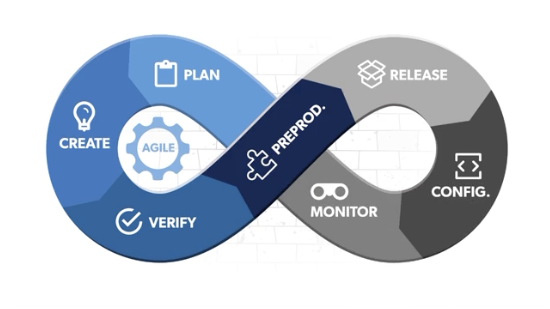
\includegraphics{png/stvAgileProcess.png}}
%\caption{\label{Figure::stvAgileProcess} PNG Image included.}
%\end{figure}

If compiling on Windows, as LaTeX-to-PDF (and not LaTeX-to-PS-to-PDF), 
you need to comment out the pdfmark package from itManual.tex:

\begin{verbatim}
%\usepackage[pdfmark, 
%breaklinks=true, 
%colorlinks=true,
%citecolor=blue,
%linkcolor=blue,
%menucolor=black,
%pagecolor=black,
%urlcolor=blue
%]{hyperref} % links in pdf
\end{verbatim}

\section{Compiling EPS files with PSFrag on Overleaf}

In the header file un-comment the following lines. (Viewable only in the .tex code, not in PDF):

	%\usepackage{graphicx} 
	%\usepackage[process=all]{pstool}
	%\usepackage[ 
	%breaklinks=true, 
	%colorlinks=true,
	%citecolor=blue,
	%linkcolor=blue,
	%menucolor=black,
	%urlcolor=blue
	%]{hyperref}
	%%%%%% 
	%%% NOTE IF LOADING hyperref PACKAGE
	%%% These lines are required ≥TL2020 due to 
	%%% incompatibility between hyperref and preview
	%%% (See https://github.com/latex3/hyperref/issues/166#issuecomment-760157370)
	%\makeatletter
	%\providecommand\HyPL@Entry[1]{}
	%\AddToHook{env/document/begin}{%
	%\@ifpackageloaded{preview}{
	%\ifPreview
		%\let\Hy@FirstPageHook\relax
		%\let\Hy@EveryPageAnchor\relax
	%\fi}{}}
	%\makeatother
	%\end{verbatim}
	%
	%\noindent
	%Then when using the image, use this syntax:
	%\begin{verbatim}
	%\begin{figure}
	%\centering
	%\psfragfig[width=1.0\linewidth]{<path to figure>}{
    %\psfrag{P0 }{\hspace{-0.5in} Test $\sum_0^N$ }
	%}
	%\caption{\label{<label name>} <Caption name>.}
	%\end{figure}

Note that with psfrag used this way, we cannot include references in the psfrag command.  
We can only replace text and use mathematical formulas.

Here is an example glossary term for \gls{should}.
\chapter[Hosts]{Hosts\\\small{\textit{-- Charles, Justin, Benedict, Jacky}}}
\label{Chapter::Hosts}
\index{Chapter!Hosts}

\begin{longtable}{|p{2.5cm}||p{5cm}||p{2.5cm}||p{6.5cm}|}
\caption{Hosts Table (Edited after Bugzilla Assignment)\label{Table::HostsTable}}\\
\hline
\textbf{Name} & \textbf{IP Address (or IP:Port)} & \textbf{OS} & \textbf{Job} \\
\hline
\endfirsthead
\hline
\textbf{Name} & \textbf{IP Address (or IP:Port)} & \textbf{OS} & \textbf{Job} \\
\hline
\endhead

devbox & 10.0.0.10 & Windows & Primary workstation used for coding and pushing commits to GitHub repositories. \\
\hline

database & 10.0.0.11 & Linux & Stores all persistent project data and connects to the backend API host. \\
\hline

testing & 10.0.0.12 & Linux & Dedicated environment for integration and regression testing prior to deployment. \\
\hline

api & 10.0.0.13 & Ubuntu 22.04 & Backend REST API server responsible for serving requests between frontend and database. \\
\hline

Bugzilla Docker & 174.138.69.132:8080 & Ubuntu & Docker container hosting Bugzilla (public HTTP access via port 8080). \\
\hline

Overleaf Docker & 104.236.74.225:80 & Ubuntu & Overleaf Community Edition instance (public HTTP access on port 80). \\
\hline

\end{longtable}

\chapter[Passwords]{Passwords\\\small{\textit{-- Charles, Justin, Benedict, Jacky}}}
\label{Chapter::Passwords}
\index{Chapter!Passwords}

\begin{longtable}{|p{3.5cm}||p{4.5cm}||p{8cm}|}
\caption{Password Table \label{Table::PasswordTable}}\\
\hline
\textbf{User / Account} & \textbf{Password (Hint)} & \textbf{Server Rules / Notes} \\
\hline
\endfirsthead
\hline
\textbf{User / Account} & \textbf{Password (Hint)} & \textbf{Server Rules / Notes} \\
\hline
\endhead

bugzilla\_admin & \texttt{<KEY><N>@bugzilla} & For the Bugzilla Docker container (\texttt{174.138.69.132:8080}). Follows the shared key rule format. \\
\hline

overleaf\_maintainer & \texttt{<KEY><N>@overleaf} & For the Overleaf Docker container (\texttt{159.65.44.227:80}). Same structure as others for maintainability. \\
\hline

api\_svc & \texttt{<KEY><N>@api} & Used by the backend API host (\texttt{10.0.0.13}). \\
\hline

db\_admin & \texttt{<KEY><N>@db} & Used for the main database host (\texttt{10.0.0.11}). \\
\hline

devbox\_admin & \texttt{<KEY><N>@devbox} & Used for the development workstation (\texttt{10.0.0.10}). \\
\hline

tester & \texttt{<KEY><N>@testing} & Used for the testing host (\texttt{10.0.0.12}). \\
\hline

\end{longtable}

\noindent
Each password follows our shared group convention: a short English word beginning and ending with the same letter (\texttt{<KEY>}), followed by a number equal to twice the number of vowels in that word (\texttt{<N>}), and ending with the site tag. This system allows easy password rotation while keeping host associations clear and consistent.

\chapter{Linux Commands \\
\small{\textit{-- Charles, Justin, Benedict, Jacky}}
\index{Linux Commands} 
\index{Chapter!Linux Commands}
\label{Chapter::Linux Commands}}

\section{Part A: Navigation \& File Ops}
\begin{itemize}
    \item 1: 
        \begin{lstlisting}[language=Python]
(base) jackylei@Jackys-MacBook-Pro lx-test % pwd
/Users/jackylei/lx-test
        \end{lstlisting}
    \item 2: 
        \begin{lstlisting}[language=Python]
(base) jackylei@Jackys-MacBook-Pro lx-test % ls -a -lh
total 136
drwxr-xr-x@ 12 jackylei  staff   384B Sep 15 16:56 .
drwxr-x---+ 58 jackylei  staff   1.8K Sep 13 22:14 ..
-rw-r--r--@  1 jackylei  staff   6.0K Sep 15 16:53 .DS_Store
drwxr-xr-x@  3 jackylei  staff    96B Sep 15 16:52 archive
-rw-r--r--@  1 jackylei  staff    48K Sep 13 22:14 blob.bin
lrwxr-xr-x@  1 jackylei  staff    13B Sep 13 22:14 link-to-file1 -> src/file1.txt
-rw-r--r--@  1 jackylei  staff     0B Sep 15 16:56 notes.md
-rw-r--r--@  1 jackylei  staff    56B Sep 15 16:56 people.csv
drwxr-xr-x@  5 jackylei  staff   160B Sep 13 22:14 src
-rw-r--r--@  1 jackylei  staff    56B Sep 13 22:14 sys.log
drwxr-xr-x@  3 jackylei  staff    96B Sep 15 16:04 tmp
-rw-r--r--@  1 jackylei  staff    28B Sep 13 22:14 words.txt
        \end{lstlisting}
    \item 3: 
        \begin{lstlisting}[language=Python]
(base) jackylei@Jackys-MacBook-Pro lx-test % [ -d tmp ] && cp -v src/file1.txt tmp
src/file1.txt -> tmp/file1.txt
        \end{lstlisting}
    \item 4: 
        \begin{lstlisting}[language=Python]
(base) jackylei@Jackys-MacBook-Pro lx-test % mv -v old.txt archive/
old.txt -> archive/old.txt
        \end{lstlisting}
    \item 5: 
        \begin{lstlisting}[language=Python]
(base) jackylei@Jackys-MacBook-Pro lx-test % touch notes.md
        \end{lstlisting}
    \item 6:     
        \begin{lstlisting}[language=Python]
(base) jackylei@Jackys-MacBook-Pro lx-test % du -h src
        \end{lstlisting}
\end{itemize}

\section{Part B: Viewing \& Searching}
\begin{itemize}
    \item 7: 
        \begin{lstlisting}[language=Python]
(base) jackylei@Jackys-MacBook-Pro lx-test % cat -n sys.log
     1	INFO boot ok
     2	WARN disk low
     3	ERROR fan fail
     4	INFO shutdown
        \end{lstlisting}
    \item 8:
        \begin{lstlisting}[language=Python]
(base) jackylei@Jackys-MacBook-Pro lx-test % cat sys.log | grep "ERROR"
ERROR fan fail
        \end{lstlisting}
    \item 9:
        \begin{lstlisting}[language=Python]
(base) jackylei@Jackys-MacBook-Pro lx-test % grep -o -i '[[:alnum:]]\+' words.txt | sort -u | wc -l
       4
        \end{lstlisting}
    \item 10:
        \begin{lstlisting}[language=Python]
(base) jackylei@Jackys-MacBook-Pro lx-test % cat words.txt | grep -i "g"
Gamma
gamma
        \end{lstlisting}
    \item 11:
        \begin{lstlisting}[language=Python]
(base) jackylei@Jackys-MacBook-Pro lx-test % head -2 people.csv
id,name,dept
1,Ada,EE
        \end{lstlisting}
    \item 12:
        \begin{lstlisting}[language=Python]
(base) jackylei@Jackys-MacBook-Pro lx-test % tail -3 sys.log
WARN disk low
ERROR fan fail
INFO shutdown
        \end{lstlisting}
\end{itemize}

\section{Part C: Text Processing}
\begin{itemize}
    \item 13: 
        \begin{lstlisting}[language=Bash]
awk -F ',' 'NR > 1 {print $2}' people.csv
        \end{lstlisting}

        \begin{figure}[H]
            \centering
            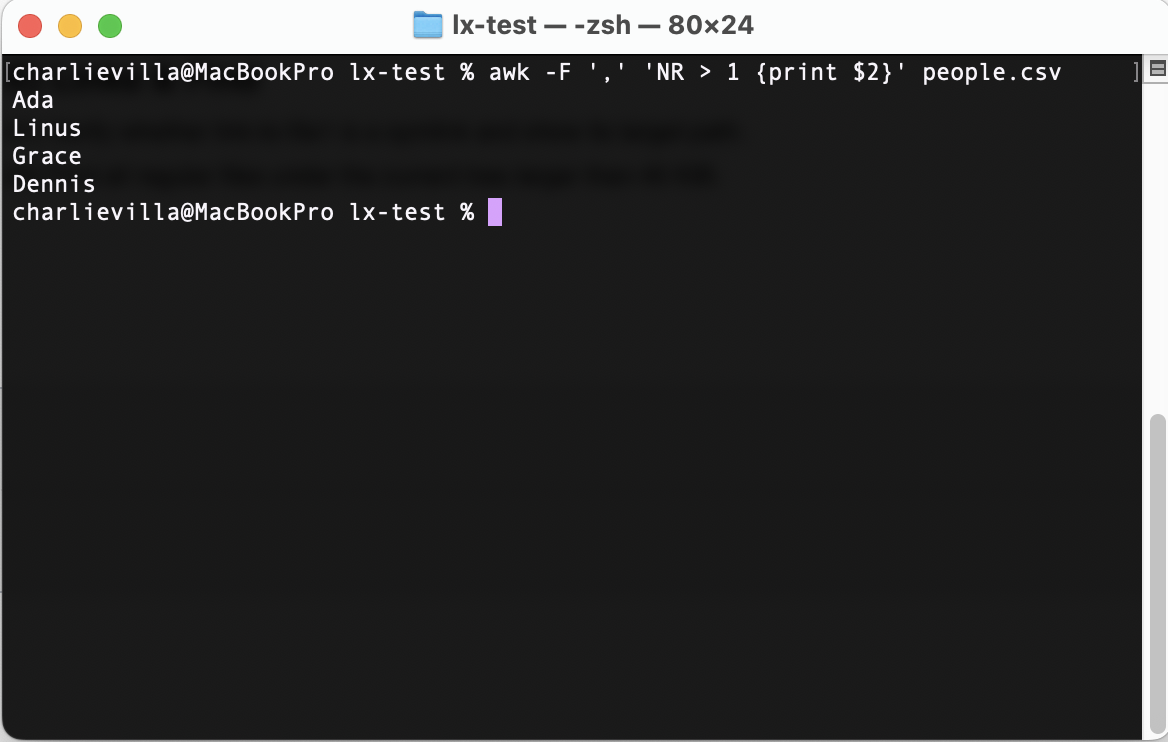
\includegraphics[width=15cm, height=10cm]{png/LinuxProblemSetPicsPNG/part_c_13.png}
            \caption{Part C \#13 Terminal Output}
            \label{fig:part C 13}
        \end{figure}
    \item 14: 
        \begin{lstlisting}[language=Bash]
sort -f -u words.txt
        \end{lstlisting}

        \begin{figure}[H]
            \centering
            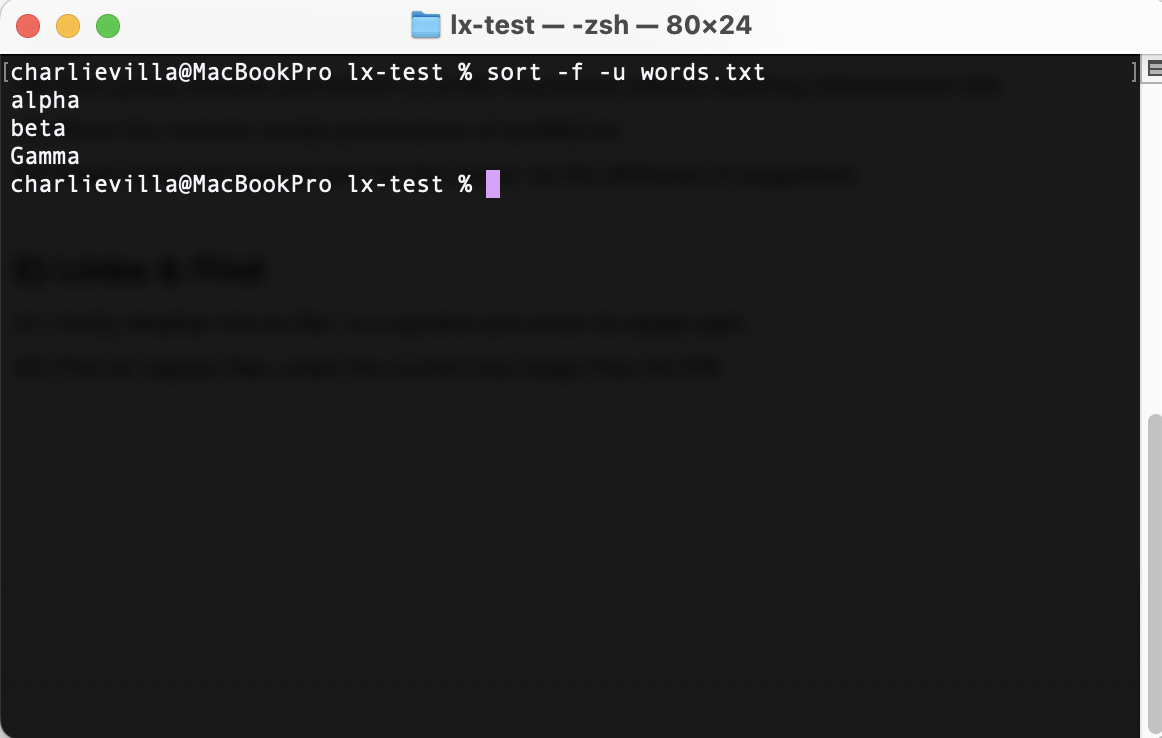
\includegraphics[width=15cm, height=10cm]{png/LinuxProblemSetPicsPNG/part_c_14.png}
            \caption{Part C \#14 Terminal Output}
            \label{fig:part C 14}
        \end{figure}
    \item 15: 
    \begin{lstlisting}[language=Bash]
find src/ -type f -exec sed -i.bak 's/three/3/g' {} +
    \end{lstlisting}

    No terminal output for question 15
    \item 16: 
        \begin{lstlisting}[language=Bash]
wc src/*.txt
        \end{lstlisting}

        \begin{figure}[H]
            \centering
            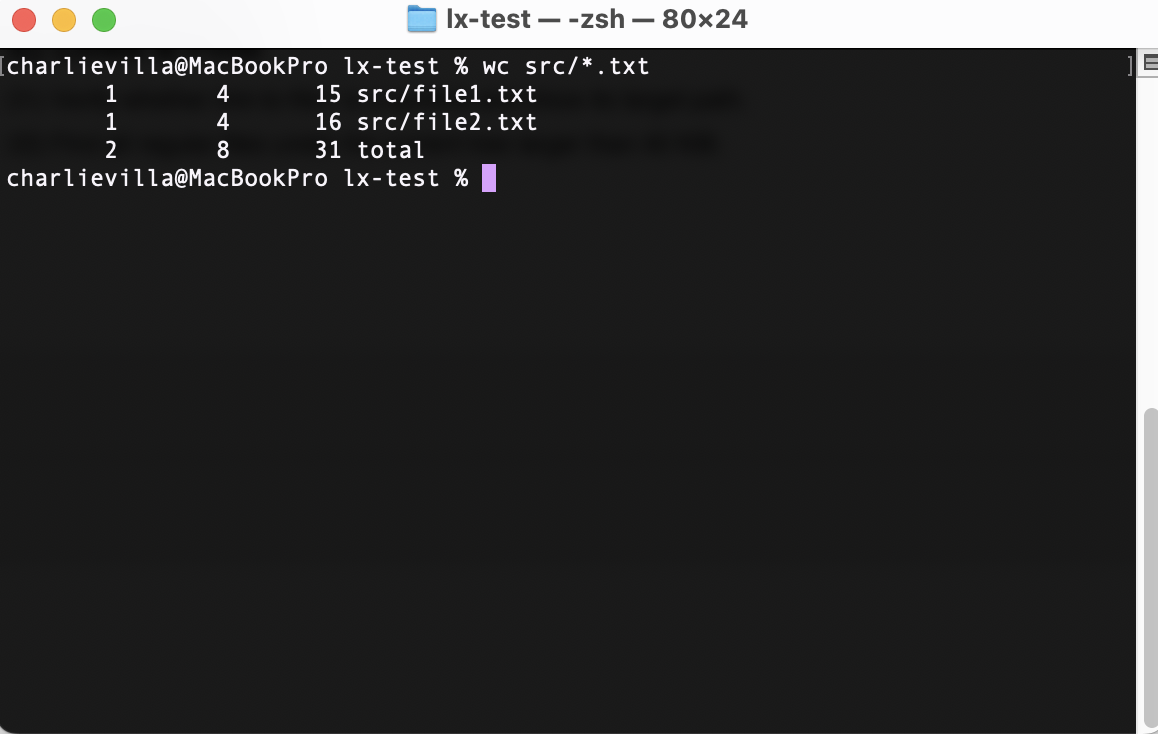
\includegraphics[width=15cm, height=10cm]{png/LinuxProblemSetPicsPNG/part_c_16.png}
            \caption{Part C \#16 Terminal Output}
            \label{fig:partC 16}
        \end{figure}
\end{itemize}

\section{Part D: Permissions \& Ownership}
\begin{itemize}
    \item 17: 
        \begin{lstlisting}[language=Bash]
chmod 700 tmp/
        \end{lstlisting}

        No terminal output for question 17
    \item 18: 
        \begin{lstlisting}[language=Bash]
chmod -R g+x src/lib
        \end{lstlisting}

        No terminal output for question 18
    \item 19: 
    \begin{lstlisting}[language=Bash]
stat -f %p src/file2.txt
    \end{lstlisting}

    \begin{figure}[H]
        \centering
        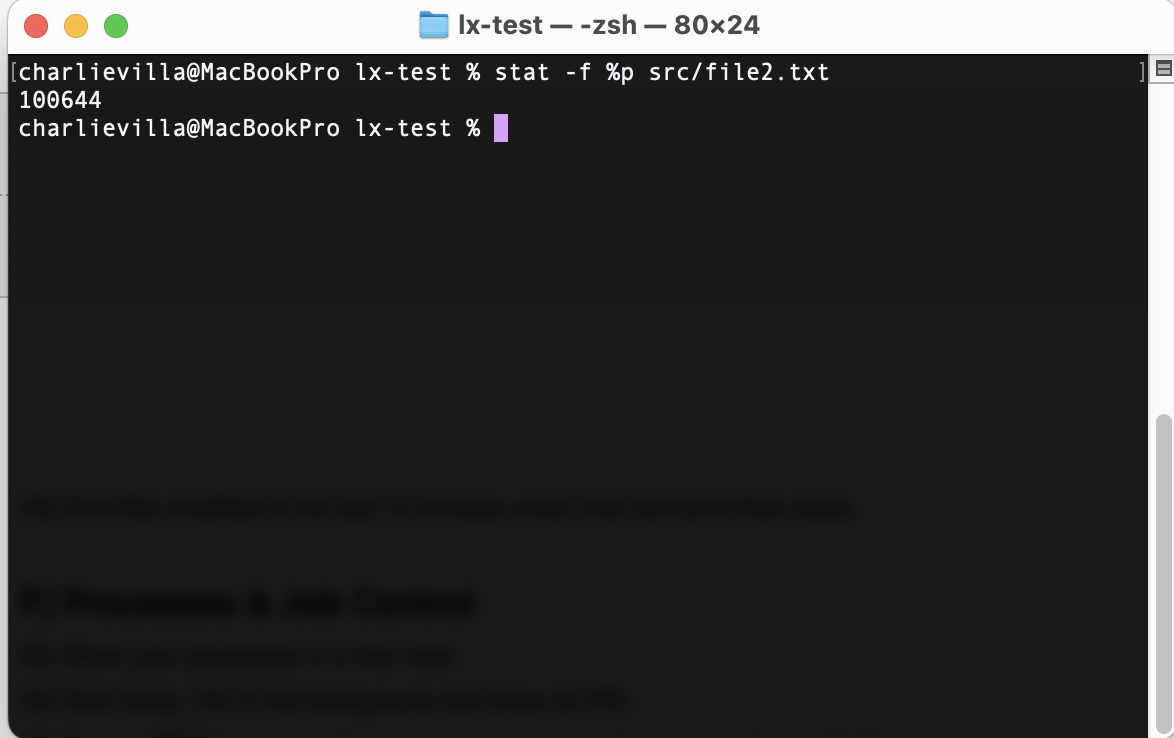
\includegraphics[width=15cm, height=10cm]{png/LinuxProblemSetPicsPNG/part_d_19.png}
        \caption{Part C \#19 Terminal Output}
        \label{fig:partC 19}
    \end{figure}
    \item 20: 
    \begin{lstlisting}[language=Bash]
touch notes.md
chflags uappnd notes.md
    \end{lstlisting}

    No terminal output for question 20
\end{itemize}

\section{Part E: Links \& Find}
\begin{itemize}
    \item 21: 
    \begin{lstlisting}[language=Bash]
ls -l link-to-file1
    \end{lstlisting}

    \begin{figure}[H]
        \centering
        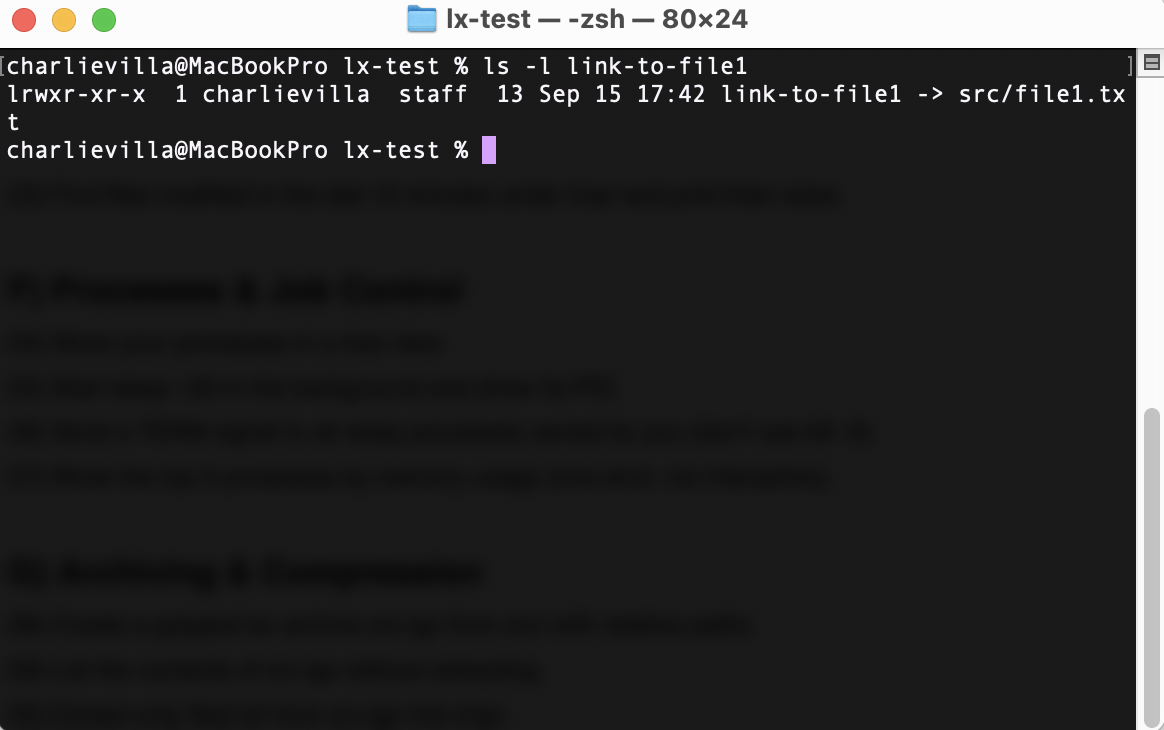
\includegraphics[width=12cm, height=7cm]{png/LinuxProblemSetPicsPNG/part_e_21.png}
        \caption{Part C \#21 Terminal Output}
        \label{fig:partC 21}
    \end{figure}    
    \item 22: 
    \begin{lstlisting}[language=Bash]
find . -type f -size +40k
    \end{lstlisting}

    \begin{figure}[H]
        \centering
        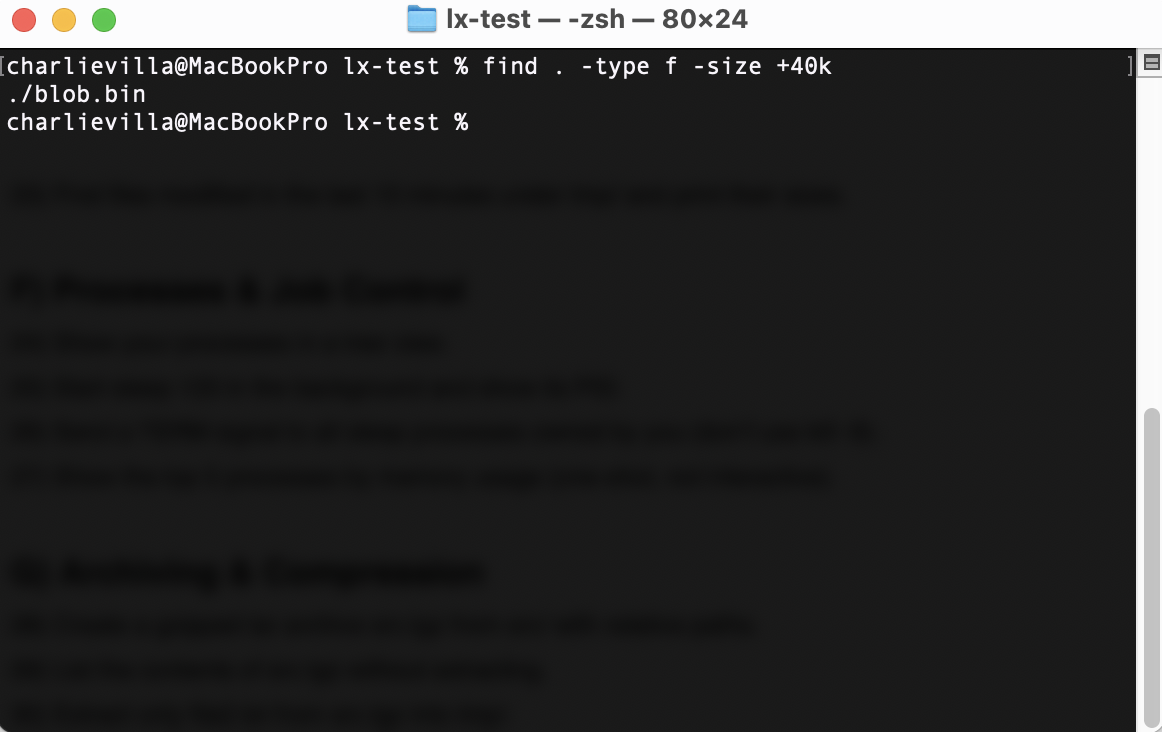
\includegraphics[width=12cm, height=7cm]{png/LinuxProblemSetPicsPNG/part_e_22.png}
        \caption{Part C \#22 Terminal Output}
        \label{fig:partC 22}
    \end{figure}  
    \item 23: 
    \begin{lstlisting}[language=Bash]
touch tmp/some-new-file.txt
find tmp/ -type f -mmin -10 -exec stat -f "%z %N" {} +
    \end{lstlisting}

    Created a new file with "touch" because the tmp/ directory was empty before it.

    \begin{figure}[H]
        \centering
        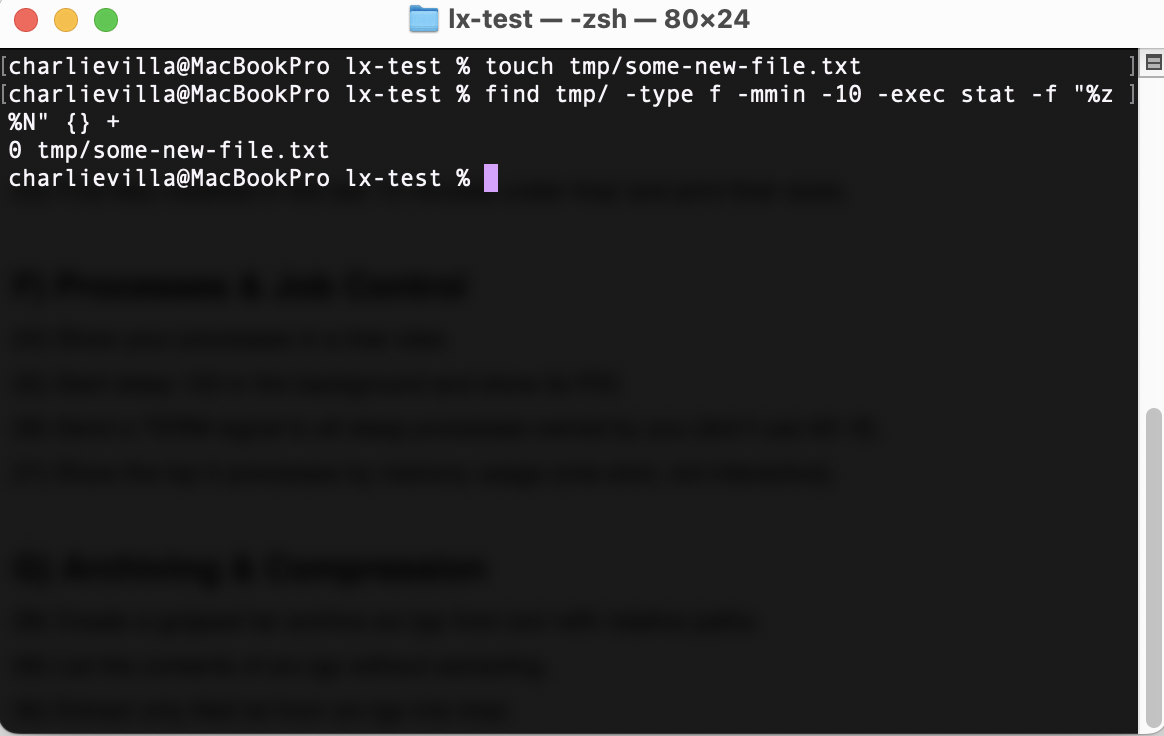
\includegraphics[width=12cm, height=7cm]{png/LinuxProblemSetPicsPNG/part_e_23.png}
        \caption{Part C \#23 Terminal Output}
        \label{fig:partC 23}
    \end{figure}  
\end{itemize}

\section{Part F: Processes \& Job Control}
\begin{itemize}
    \item 24: Tree View:
    \begin{figure}[H]
        \centering
        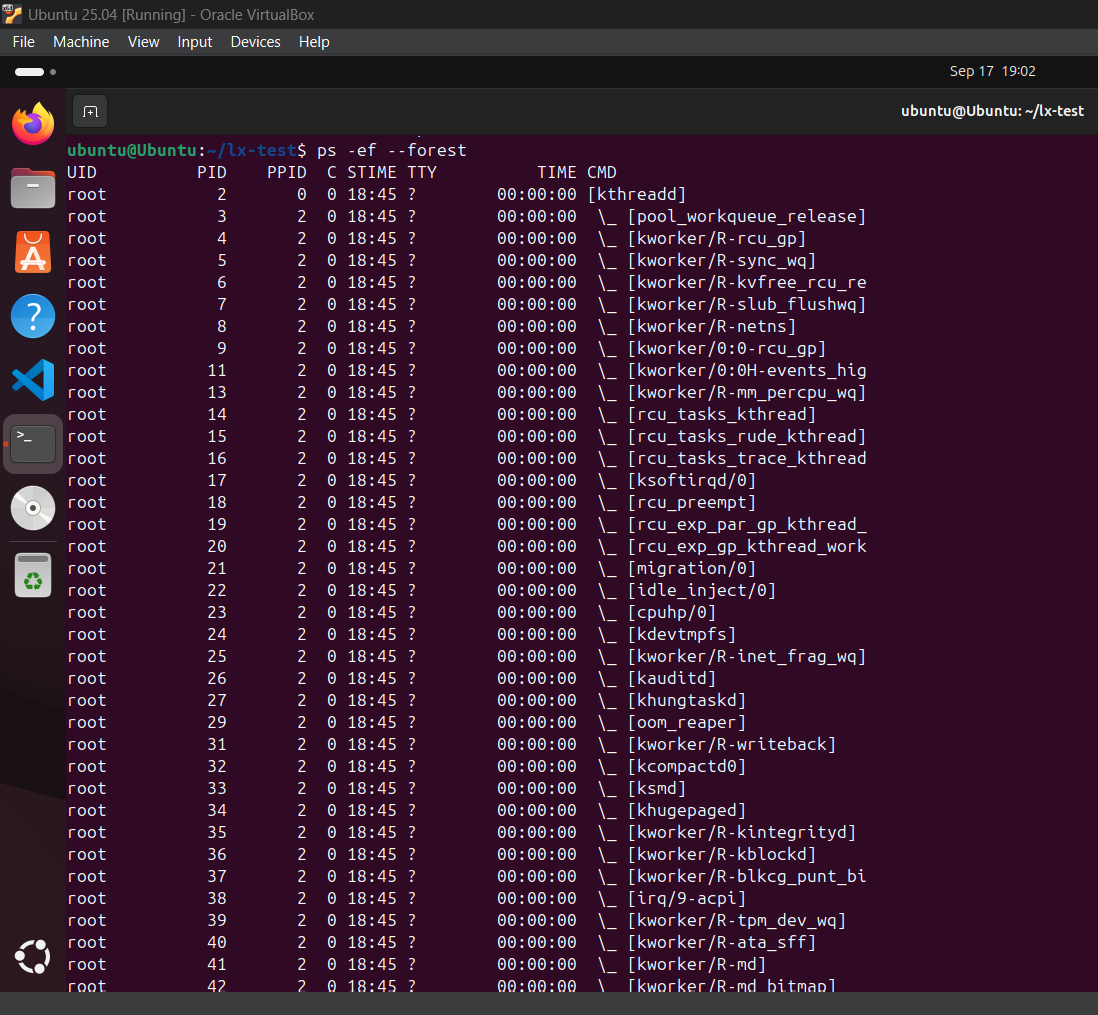
\includegraphics[width=15cm, height=10cm]{png/LinuxProblemSetPicsPNG/TreeView1.png}
        \caption{Part F \#24 Tree View 1}
        \label{fig:partF 24 Tree 1}
    \end{figure}
    \begin{figure}[H]
        \centering
        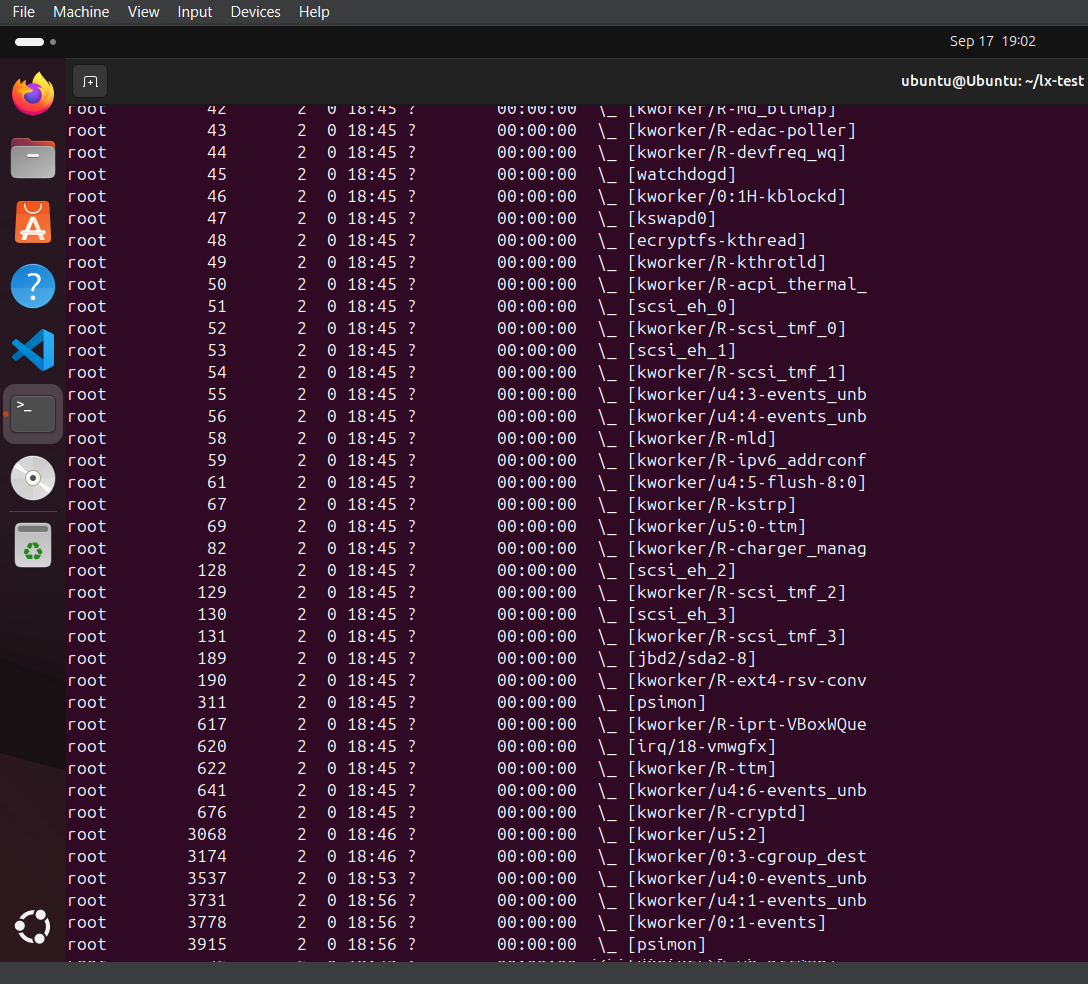
\includegraphics[width=15cm, height=10cm]{png/LinuxProblemSetPicsPNG/TreeView2.png}
        \caption{Part F \#24 Tree View 2}
        \label{fig:partF 24 Tree 2}
    \end{figure}
    \begin{figure}[H]
        \centering
        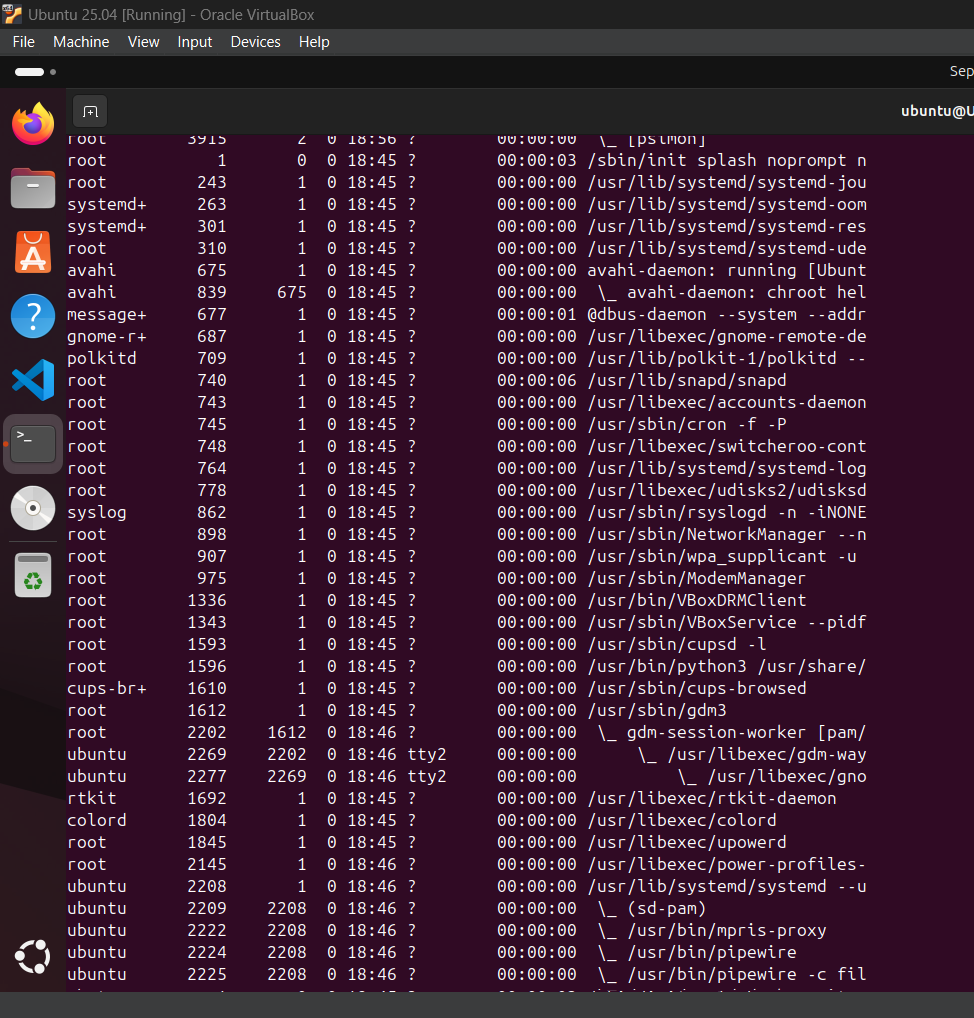
\includegraphics[width=15cm, height=10cm]{png/LinuxProblemSetPicsPNG/TreeView3.png}
        \caption{Part F \#24 Tree View 3}
        \label{fig:partF 24 Tree 3}
    \end{figure}
    \begin{figure}[H]
        \centering
        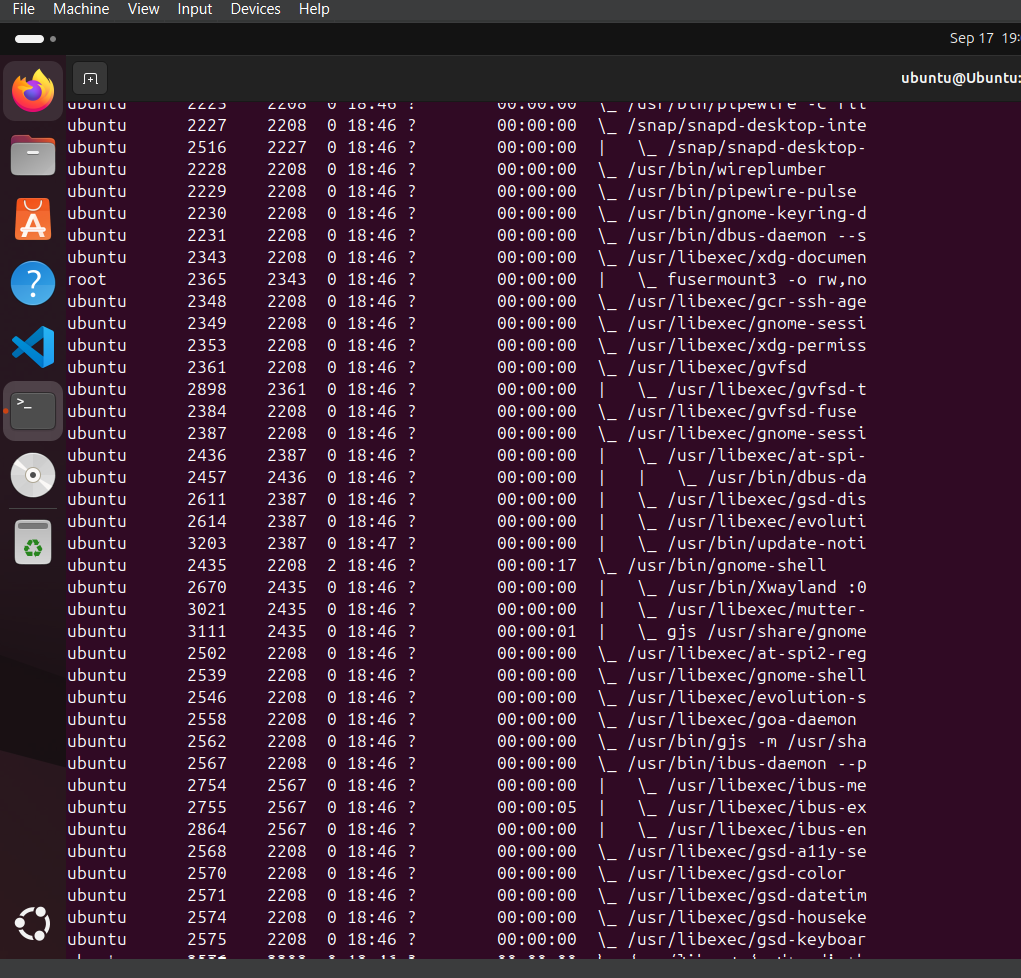
\includegraphics[width=15cm, height=10cm]{png/LinuxProblemSetPicsPNG/TreeView4.png}
        \caption{Part F \#24 Tree View 4}
        \label{fig:partF 24 Tree 4}
    \end{figure}
    \begin{figure}[H]
        \centering
        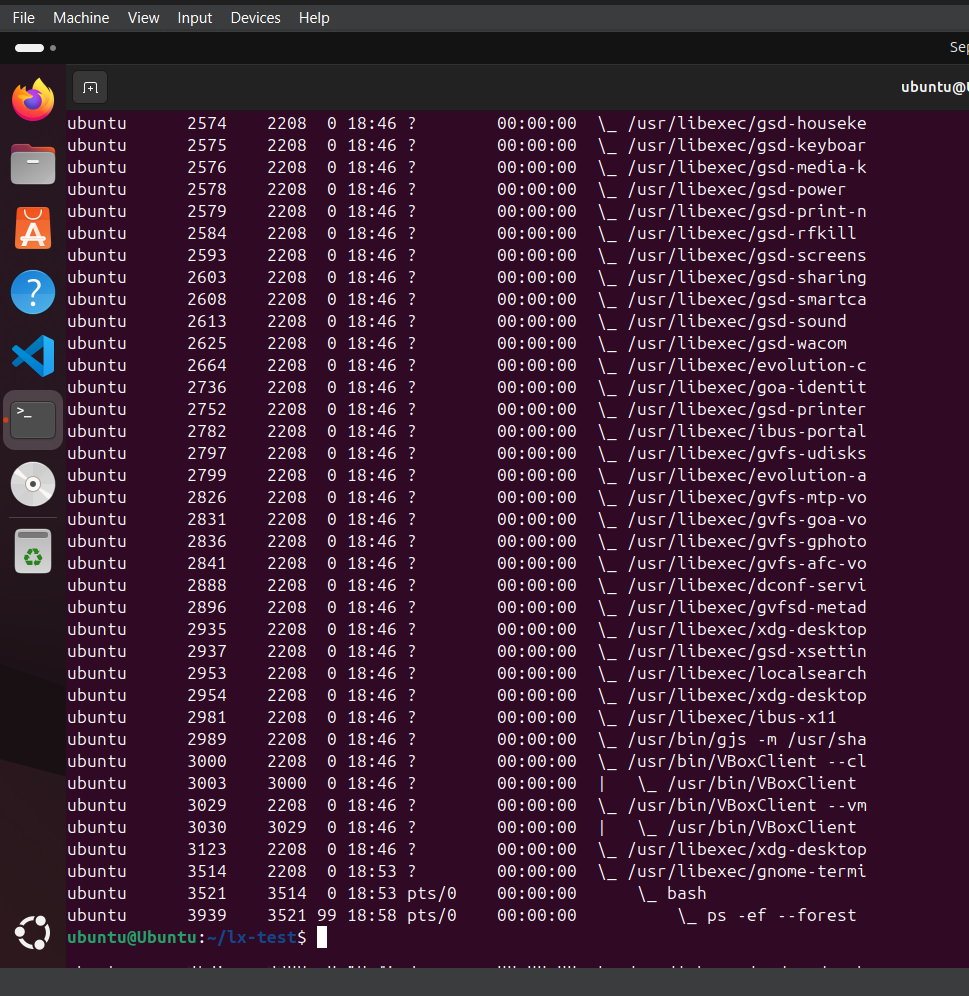
\includegraphics[width=15cm, height=10cm]{png/LinuxProblemSetPicsPNG/TreeView5.png}
        \caption{Part F \#24 Tree View 5}
        \label{fig:partF 24 Tree 5}
    \end{figure}
    
    \item 25: 
     \begin{figure}[H]
        \centering
        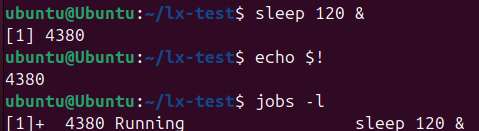
\includegraphics[width=10cm, height=5cm]{png/LinuxProblemSetPicsPNG/PartF25.png}
        \caption{Part F \#25 Sleep 120 in the background and its PID}
        \label{fig:partF 25}
    \end{figure}
    
    \item 26: 
    \begin{figure}[H]
        \centering
        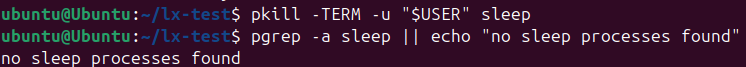
\includegraphics[width=15cm, height=4cm]{png/LinuxProblemSetPicsPNG/PartF26.png}
        \caption{Part F \#26 TERM signal}
        \label{fig:partF 26}
    \end{figure}
    
    \item 27: 
     \begin{figure}[H]
        \centering
        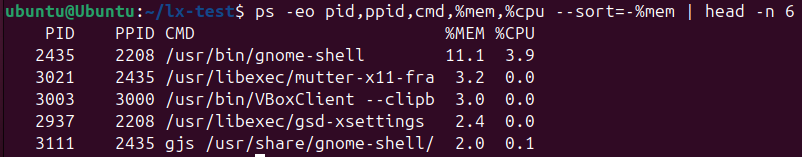
\includegraphics[width=15cm, height=4cm]{png/LinuxProblemSetPicsPNG/PartF27.png}
        \caption{Part F \#27 Top 5 Processes}
        \label{fig:partF 27}
    \end{figure}
\end{itemize}

\section{Part G: Archiving \& Compression}
\begin{itemize}
    \item 28: 
    \begin{lstlisting}[language=Bash]
        tar czf src.tar.gz
    \end{lstlisting}
    \item 29: 
    \begin{lstlisting}[language=Bash]
        tar -tf src.tar.gz
    \end{lstlisting}
    \item 30: 
    \begin{lstlisting}[language=Bash]
        tar -xzf src.tar.gz -C tmp src/file2.txt
    \end{lstlisting}
    \begin{figure}[htp]
    \centering
    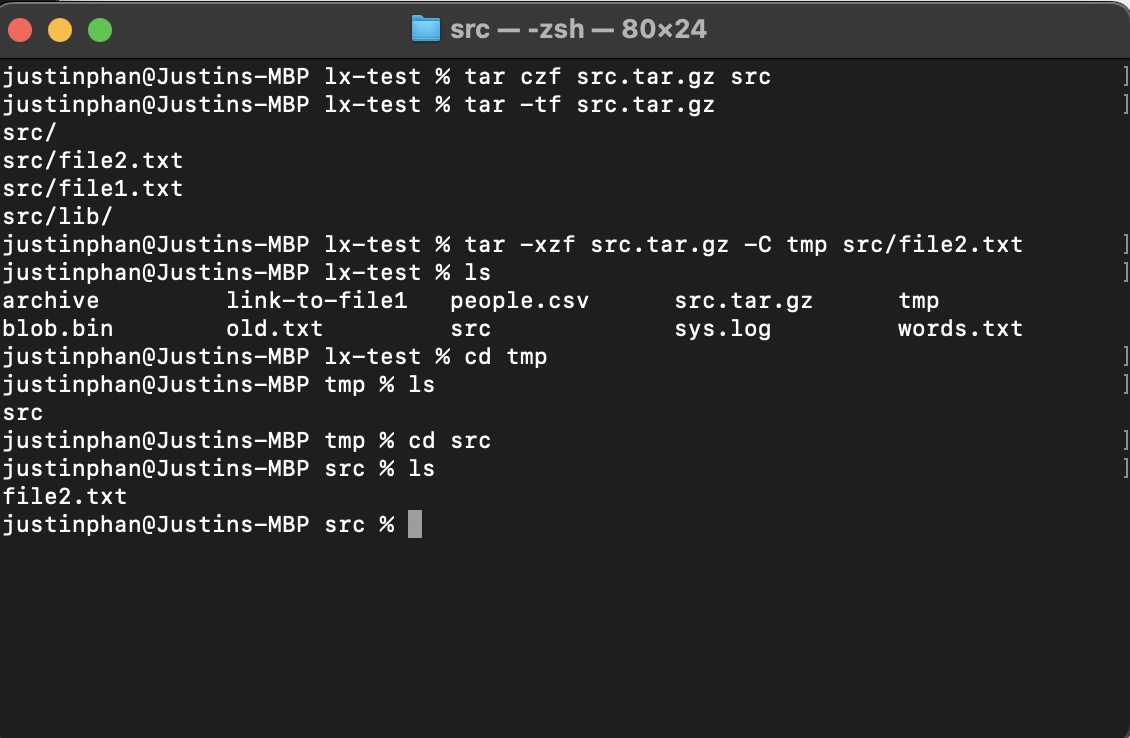
\includegraphics[width=15cm, height=10cm]{png/LinuxProblemSetPicsPNG/part_g.png}
    \caption{Part G Terminal Output}
    \label{fig:part G}
\end{figure}
\end{itemize}

\section{Part H: Networking \& System Info}
\begin{itemize}
    \item 31:
     \begin{figure}[H]
        \centering
        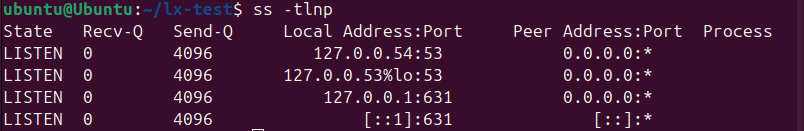
\includegraphics[width=15cm, height=4cm]{png/LinuxProblemSetPicsPNG/PartH31.png}
        \caption{Part H \#31 TCP sockets with associated PIDs }
        \label{fig:partH 31}
    \end{figure}
    
    \item 32: 
     \begin{figure}[H]
        \centering
        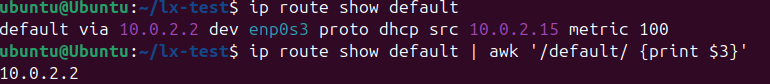
\includegraphics[width=15cm, height=4cm]{png/LinuxProblemSetPicsPNG/PartH32.png}
        \caption{Part H \#32 Default Route (gateway) in a concise form}
        \label{fig:partH 32}
    \end{figure}
    
    \item 33: 
     \begin{figure}[H]
        \centering
        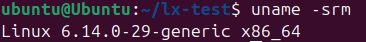
\includegraphics[width=15cm, height=4cm]{png/LinuxProblemSetPicsPNG/PartH33.png}
        \caption{Part H \#33 Kernel name, Release, and Machine Architecture}
        \label{fig:partH 33}
    \end{figure}
    
    \item 34: 
     \begin{figure}[H]
        \centering
        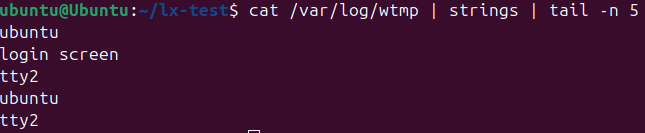
\includegraphics[width=15cm, height=4cm]{png/LinuxProblemSetPicsPNG/PartH34.png}
        \caption{Part H \#34 Last 5 successful logins on the system}
        \label{fig:partH 34}
    \end{figure}

\end{itemize}

\section{Part I: Package \& Services (Debian/Ubuntu)}
\begin{itemize}
    \item 35: 
    \begin{lstlisting}[language=Bash]
         brew list --versions coreutils
    \end{lstlisting}
    \begin{figure}[htp]
    \centering
    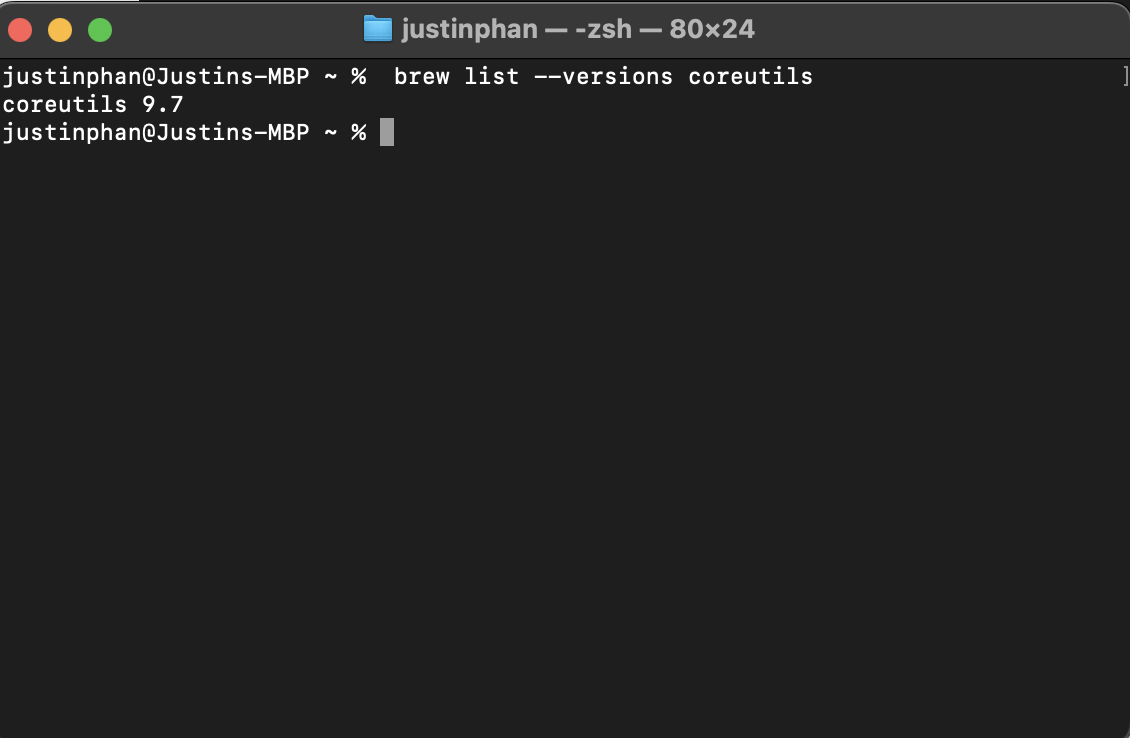
\includegraphics[width=15cm, height=10cm]{png/LinuxProblemSetPicsPNG/part_i_35.png}
    \caption{Part I \#35 Terminal Output showing the installed version of package coreutils}
    \label{fig:part I 35}
\end{figure}
    \item 36: 
    \begin{lstlisting}[language=Bash]
        brew search ripgrep
    \end{lstlisting}
    \begin{figure}[htp]
    \centering
    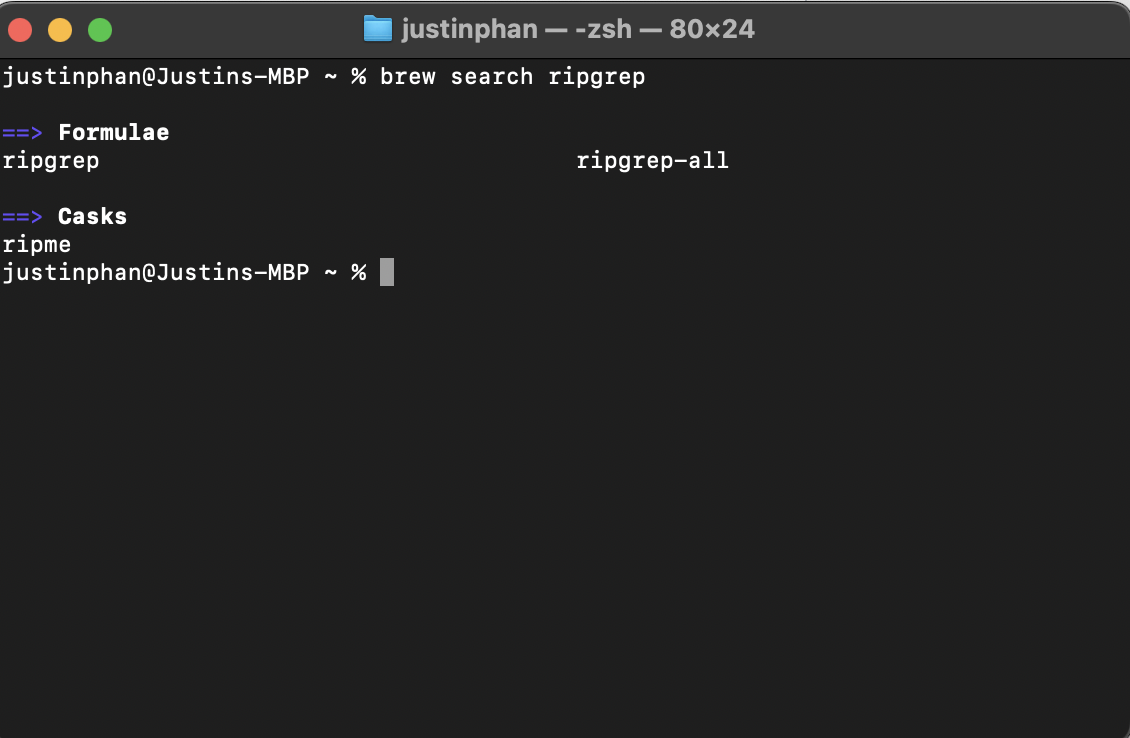
\includegraphics[width=15cm, height=10cm]{png/LinuxProblemSetPicsPNG/part_i_36.png}
    \caption{Part I \#36 Terminal Output showing all available packages whose names contain ripgrep}
    \label{fig:part I 36}
\end{figure}
    \item 37: 
    \begin{lstlisting}[language=Bash]
        systemctl status cron | grep "Active."
    \end{lstlisting}
    \begin{figure}[htp]
    \centering
    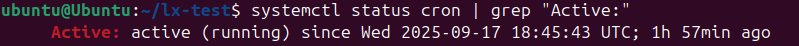
\includegraphics[width=16cm, height=4cm]{png/LinuxProblemSetPicsPNG/part_i_37.png}
    \caption{Part I \#37 Terminal Output}
    \label{fig:part I 37}
\end{figure}
\end{itemize}

\section{Part J: Bash \& Scripting}
\begin{itemize}
    \item 38: 
     \begin{figure}[H]
        \centering
        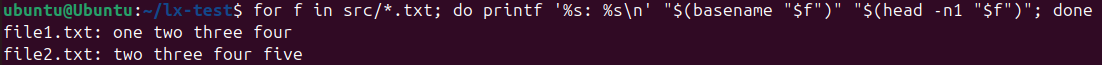
\includegraphics[width=12cm, height=2cm]{png/LinuxProblemSetPicsPNG/PartI38.png}
        \caption{Part J \#38 One-liner that loops over}
        \label{fig:partJ 38}
    \end{figure}
    \item 39: 
     \begin{figure}[H]
        \centering
        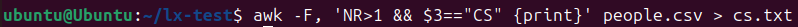
\includegraphics[width=15cm, height=2cm]{png/LinuxProblemSetPicsPNG/PartI39.png}
        \caption{Part J \#39 A command that exports CSV rows}
        \label{fig:partJ 39}
    \end{figure}
    \item 40: 
     \begin{figure}[H]
        \centering
        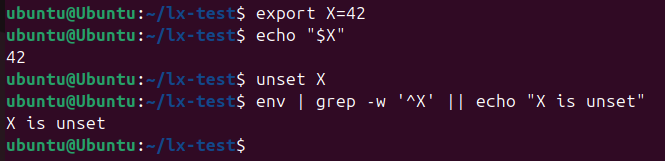
\includegraphics[width=15cm, height=4cm]{png/LinuxProblemSetPicsPNG/PartI40.png}
        \caption{Part J \#40 Create a variable X with value 42}
        \label{fig:partJ 40}
    \end{figure}
\end{itemize}


\chapter[Project Proposal]{Project Proposal\\\small{\textit{-- Charles, Justin, Benedict, Jacky}}}
\label{Chapter::Project Proposal}
\index{Chapter!Project Proposal}

% Please describe your project.
% Include a title and a description that includes sample task and DevSecOps tools used, such as source control, testing, deployment, databases, etc.  At this point everything is very vague, but I want you to think about the tools you might need, even if you don't have all the tools very detailed yet.
% 2. Expectations/Rubric for the project:

% The project will be evaluated based on:

% Selected tool, tools or environment
% Building a sample working application (40 pts)
% Using specific tools (DevOps tools) to build a simple project. 
% Ideally, you will try using two comparable tools to do the same project and draw comparisons (security, development, hosting, monitoring, testing, operations, …) (20 pts)
% Use an environment to build the project, AWS, azure or homebrew (containers, micro services, github, …) (20 pts)
% Construct a dashboard reflecting operational aspects (20 pts)
% Construct a modified strength, weakness, opportunities, thread (SWOT) chart for each tool (20 pts)
% Propose something unique


\textbf{Project Title:} Dicey DevOps: A Luck-Based Probability Game
\\

\textbf{Project Description:} Our project is a web-based luck game that also teaches concepts of probability and the idea of risk versus reward. Players will roll dice and place bets on different outcomes such as totals, pairs, triples, or exact numbers. They can choose to re-roll or lock dice, which adds strategic choices between safer but lower-value options and riskier plays with higher potential rewards. The game will also feature occasional "event rounds" where special conditions apply (such as bonus payouts or inverted win conditions). After each round, the game will provide insights into the actual probability of success and expected value, helping players better understand chance, statistics, and decision-making.

Sample tasks include designing the dice roll system with fair randomness, building a leader board to track high scores, and implementing "learning mode" features that explain probabilities to the player. Some tasks we have brainstormed include implementing the dice roll system, building a leader board, and creating a "learning mode" that explains probability insights to players. We will also design a dashboard to track both system health and game-related metrics such as win/loss ratios, re-roll usage, and outcome distributions.

For the DevOps side, we plan to use version control, testing, deployment pipelines, and monitoring tools. Examples may include GitHub for source control, Gitlab CI/CD pipelines to automate builds and deployments, PostgreSQL or another database for storing results, containerization with Docker, infrastructure as code tools for environment setup, and monitoring solutions such as Prometheus and Grafana. We are still discussing the exact tech stack as a team, but our goal is to keep the setup lightweight and easy to extend while still allowing us to compare multiple DevOps tools as required.


\chapter[AWS Deployment]{AWS Deployment\\\small{\textit{-- Charles, Justin, Benedict, Jacky}}}
\label{Chapter::AWS Deployment}
\index{Chapter!AWS Deployment}

\noindent\textbf{Live URL:} \url{https://zjnbvfjpug.us-east-1.awsapprunner.com}

\section*{Overview}
We deployed the \emph{Two Buttons} website as a containerized service on AWS. The pipeline is:
\begin{enumerate}
  \item Authenticate the AWS CLI via \textbf{SSO} (IAM Identity Center).
  \item Build a Docker image locally and push it to \textbf{Amazon ECR}.
  \item Deploy from ECR to a managed container runtime using \textbf{AWS App Runner}.
\end{enumerate}

\paragraph{Why App Runner?}
For a small stateless web app, App Runner removes the need to manage ECS tasks/services, load balancers, or EC2 capacity. It auto-builds or pulls from ECR, provisions HTTPS and scaling, and exposes a public URL with minimal ops overhead (good for a course project).

\paragraph{Project root used for the build}
\path{C:\Users\benma\Documents\docker-examples-benedict\docker-examples\color-buttons-app}

\subsection*{Prerequisites}
\begin{itemize}
  \item Windows 10/11 with \textbf{Docker Desktop} and \textbf{AWS CLI v2}.
  \item \textbf{SSO} set up in the AWS Console (IAM Identity Center) with an AdminAccess permission set (temporary for the lab).
  \item Overleaf configured to compile with \texttt{minted} (shell escape enabled).
\end{itemize}

\section*{Authenticate the AWS CLI (SSO)}
\begin{minted}[fontsize=\small]{powershell}
aws configure sso
aws sso login --profile default
aws sts get-caller-identity --profile default
# Confirm the returned Account ID is yours and an SSO role is assumed.
\end{minted}

\section*{Build, Tag, and Push the Image to Amazon ECR}
\vspace{-0.5\baselineskip}
\begin{minted}[fontsize=\small]{powershell}
# Go to the project folder
cd "C:\Users\benma\Documents\docker-examples-benedict\docker-examples\color-buttons-app"

# Environment
$Env:AWS_REGION="us-east-1"
$Env:ECR_REPO="color-buttons-app"
$Env:IMAGE_TAG="v1"
$Env:AWS_ACCOUNT_ID=(aws sts get-caller-identity --query Account --output text --profile default)

# Create the ECR repo if missing
aws ecr describe-repositories --repository-names $Env:ECR_REPO --region $Env:AWS_REGION --profile default *> $null ; if ($LASTEXITCODE -ne 0) {
  aws ecr create-repository --repository-name $Env:ECR_REPO `
    --image-scanning-configuration scanOnPush=true `
    --region $Env:AWS_REGION --profile default
}

# Log in Docker to ECR
aws ecr get-login-password --region $Env:AWS_REGION --profile default |
  docker login --username AWS --password-stdin "$($Env:AWS_ACCOUNT_ID).dkr.ecr.$($Env:AWS_REGION).amazonaws.com"

# Build, tag, and push (force linux/amd64 for App Runner build fleet compatibility)
docker build --platform linux/amd64 -t "$($Env:ECR_REPO):$($Env:IMAGE_TAG)" .
docker tag  "$($Env:ECR_REPO):$($Env:IMAGE_TAG)" `
            "$($Env:AWS_ACCOUNT_ID).dkr.ecr.$($Env:AWS_REGION).amazonaws.com/$($Env:ECR_REPO):$($Env:IMAGE_TAG)"
docker push "$($Env:AWS_ACCOUNT_ID).dkr.ecr.$($Env:AWS_REGION).amazonaws.com/$($Env:ECR_REPO):$($Env:IMAGE_TAG)"
\end{minted}

\section*{Deploy with AWS App Runner (Console)}
\begin{enumerate}
  \item \textbf{Create service} $\rightarrow$ \textbf{Source}: \emph{Container registry} $\rightarrow$ \emph{Amazon ECR}.\\
        Choose repository \texttt{color-buttons-app} and tag \texttt{v1}.
  \item \textbf{Service name}: \texttt{color-buttons-app} \quad \textbf{Port}: \texttt{3000}.
  \item \textbf{ECR access role}: \emph{Create new service role} (let App Runner pull from ECR).
  \item \textbf{Health check}: \texttt{HTTP} on path \texttt{/} (timeout 5s, interval 10s).
  \item Click \textbf{Create \& Deploy}; wait for \emph{Status: Running} and note the \emph{Default domain}.
\end{enumerate}

\section*{Verification}
\begin{minted}[fontsize=\small]{powershell}
# Expect HTTP/2 200 (or similar)
curl -I https://zjnbvfjpug.us-east-1.awsapprunner.com
\end{minted}
Manually verify the page renders and both buttons switch background color (blue/red).

\section*{Operating the Service (Logs, Scaling, Rollback)}
\begin{itemize}
  \item \textbf{Logs:} In App Runner $\rightarrow$ \emph{Logs} tab to view system/app logs.
  \item \textbf{Scaling:} Default concurrency is 100 requests/instance, min 1, max 25 instances.
  \item \textbf{Re-deploy:} Push the same tag and choose \emph{Actions $\rightarrow$ Deploy} for manual trigger services.
  \item \textbf{Rollback:} Keep prior image tags; re-point the service to the last known-good tag and redeploy.
\end{itemize}

\section*{Cost Guardrails \& Cleanup}
App Runner and ECR are pay-as-you-go. To avoid charges after grading:
\begin{enumerate}
  \item In \textbf{App Runner}: \emph{Actions $\rightarrow$ Pause} or \emph{Delete} the service.
  \item In \textbf{ECR}: delete the image(s) and (optionally) the repository.
\end{enumerate}
(We also set an AWS Budget alarm earlier to notify on any unexpected spend.)

\section*{Figure}
\begin{figure}[htbp]
  \centering
  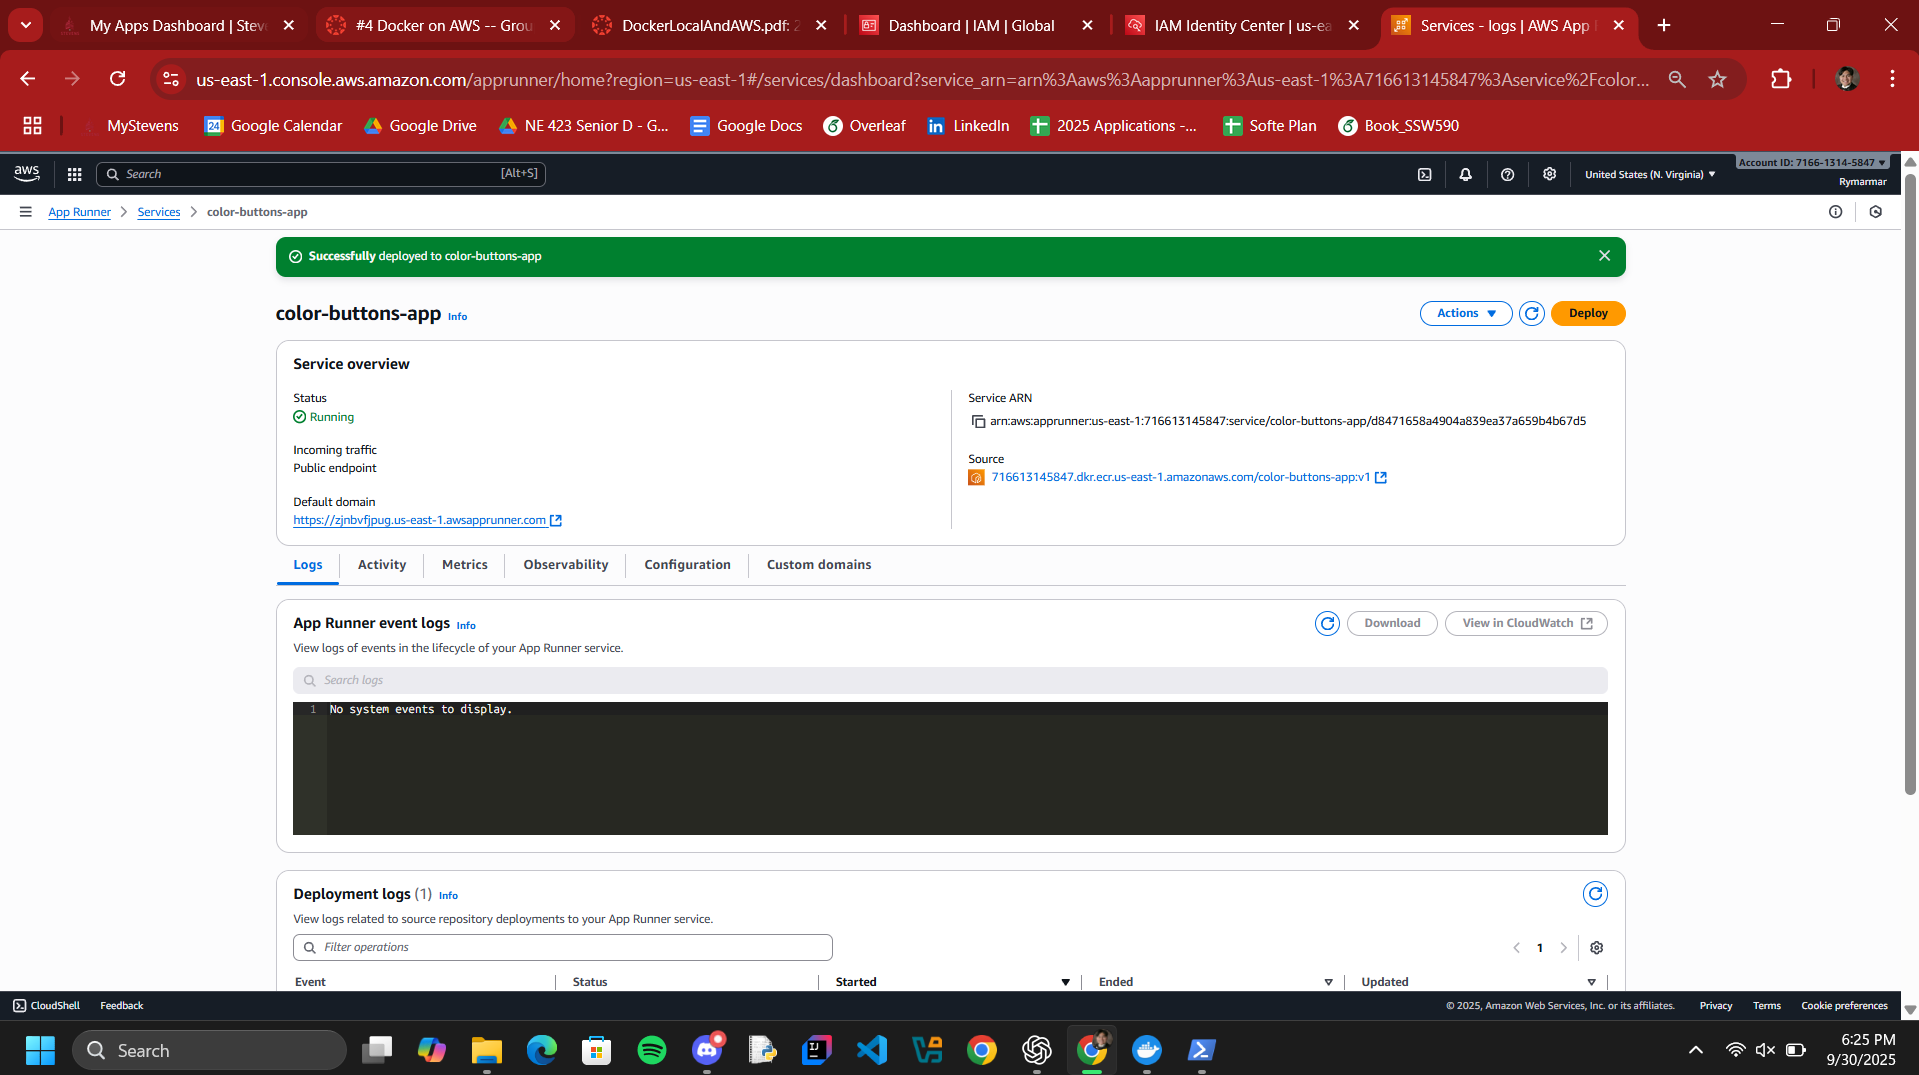
\includegraphics[width=.95\linewidth]{png/docker/app-runner-running.png}
  \caption{App Runner service in \emph{Running} state with the default domain.}
\end{figure}

\section*{Class-based JavaScript Refactor}

We replaced the old function-based handlers with an class that encapsulates all behavior (buttons, events, and background updates). Only the public assets changed (\texttt{public/index.html}, \texttt{public/app.js}); the server continues to serve \texttt{public/} and listen on \texttt{0.0.0.0:3000}.

\subsection*{Updated \texttt{public/index.html}}
\begin{minted}[fontsize=\small]{html}
<!doctype html>
<html lang="en">
<head>
  <meta charset="utf-8" />
  <title>Two Buttons</title>
</head>
<body>
  <h1>Two Buttons</h1>
  <button id="blueBtn">Blue</button>
  <button id="redBtn">Red</button>

  <script src="app.js"></script>
</body>
</html>
\end{minted}

\subsection*{New \texttt{public/app.js} (class-based)}
\begin{minted}[fontsize=\small]{javascript}
class ColorButtonsApp {
  constructor() {
    this.$blue = document.getElementById("blueBtn");
    this.$red  = document.getElementById("redBtn");
    this.bindEvents();
  }
  bindEvents() {
    this.$blue.addEventListener("click", () => this.setBg("steelblue"));
    this.$red .addEventListener("click", () => this.setBg("crimson"));
  }
  setBg(color) { document.body.style.backgroundColor = color; }
}
window.addEventListener("DOMContentLoaded", () => new ColorButtonsApp());
\end{minted}

\begin{figure}[htbp]
  \centering
  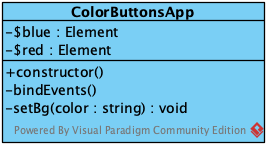
\includegraphics[width=.95\linewidth]{png/docker/DockerOnAWSGroup.png}
  \caption{Class Diagram for App.js}
\end{figure}

\subsection*{Server.js}
\begin{minted}[fontsize=\small]{javascript}
import express from "express";
import path from "path";
import { fileURLToPath } from "url";

const __filename = fileURLToPath(import.meta.url);
const __dirname = path.dirname(__filename);

const app = express();
const PORT = process.env.PORT || 3000;

// Serve static files from public/
app.use(express.static(path.join(__dirname, "public")));

app.listen(PORT, "0.0.0.0", () => {
  console.log(`Server running at http://0.0.0.0:${PORT}!`);
});
\end{minted}

\subsection*{\texttt{package.json}}
\begin{minted}[fontsize=\small]{json}
{
  "name": "color-buttons-app",
  "version": "1.0.0",
  "type": "module",
  "main": "server.js",
  "scripts": {
    "start": "node server.js"
  },
  "dependencies": {
    "express": "^4.18.2"
  }
}
\end{minted}

\paragraph{Result.}
Clicking \textbf{Blue} or \textbf{Red} now triggers methods on a single \texttt{ColorButtonsApp} instance, keeping the global scope clean and making the behavior easy to unit test or extend.

\chapter[LaTeX Docker]{LaTeX Docker\\\small{\textit{-- Charles, Justin, Benedict, Jacky}}}
\label{Chapter::LaTeX Docker}
\index{Chapter!LaTeX Docker}



\subsection{Project Directory Setup}
\begin{itemize}
    \item Create a folder docker-latex 
    \item Start docker
    \item Make sure docker is running by using docker run hello-world 
    \item cd into that folder directory 
\end{itemize}

\subsection{Docker Commands}
\begin{itemize}
    \item Create a Dockerfile with the content below
\end{itemize}

\begin{minted}{Bash}
FROM debian:bullseye-slim

ENV DEBIAN_FRONTEND=noninteractive

RUN apt-get update && \
    apt-get install -y \
        texlive-latex-base \
        texlive-latex-recommended \
        texlive-fonts-recommended \
        texlive-latex-extra \
        make \
        && apt-get clean && rm -rf /var/lib/apt/lists/*

WORKDIR /doc

CMD ["pdflatex", "main.tex"]
\end{minted}
\begin{itemize}
    \item Run nano main.tex and paste your desired LaTeX content 
    \item Build the docker image 
    \item Run the docker command 
    \item Check your folder to see if the main.pdf file is created 
\end{itemize}

\begin{minted}{Bash}
    nano main.tex
    docker build -t docker-latex . 
    docker run --rm -v "$PWD":/doc docker-latex
\end{minted}

\begin{figure}[htp]
    \centering
    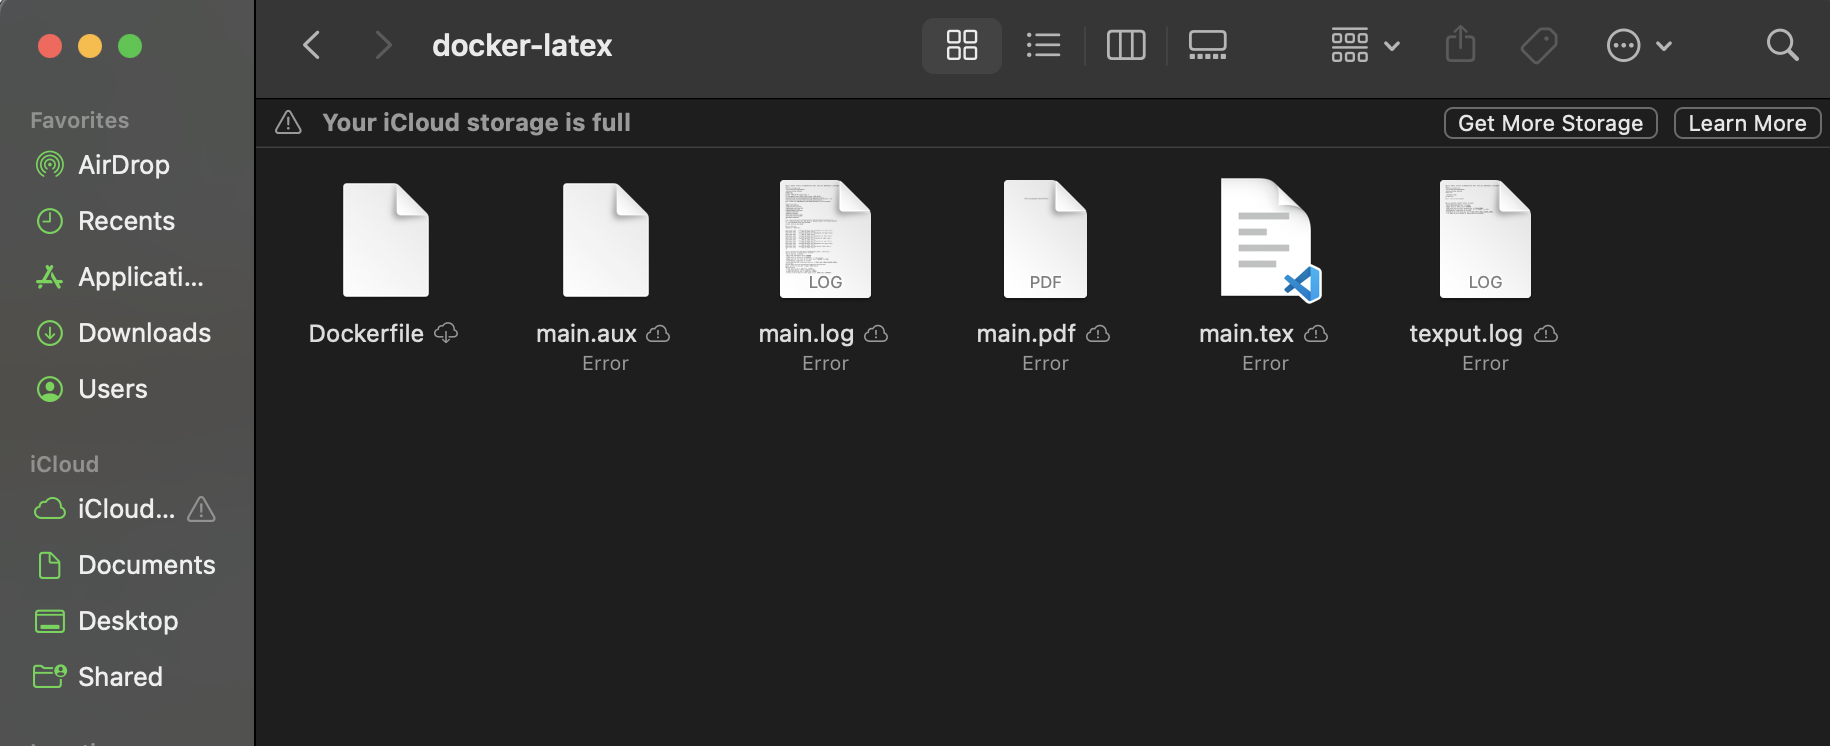
\includegraphics[width=15cm, height=10cm]{png/docker/docker-latex.png}
    \caption{Folder containing files created from successful Docker build}
    \label{fig:Part I Folder}
\end{figure}

\begin{figure}[htp]
    \centering
    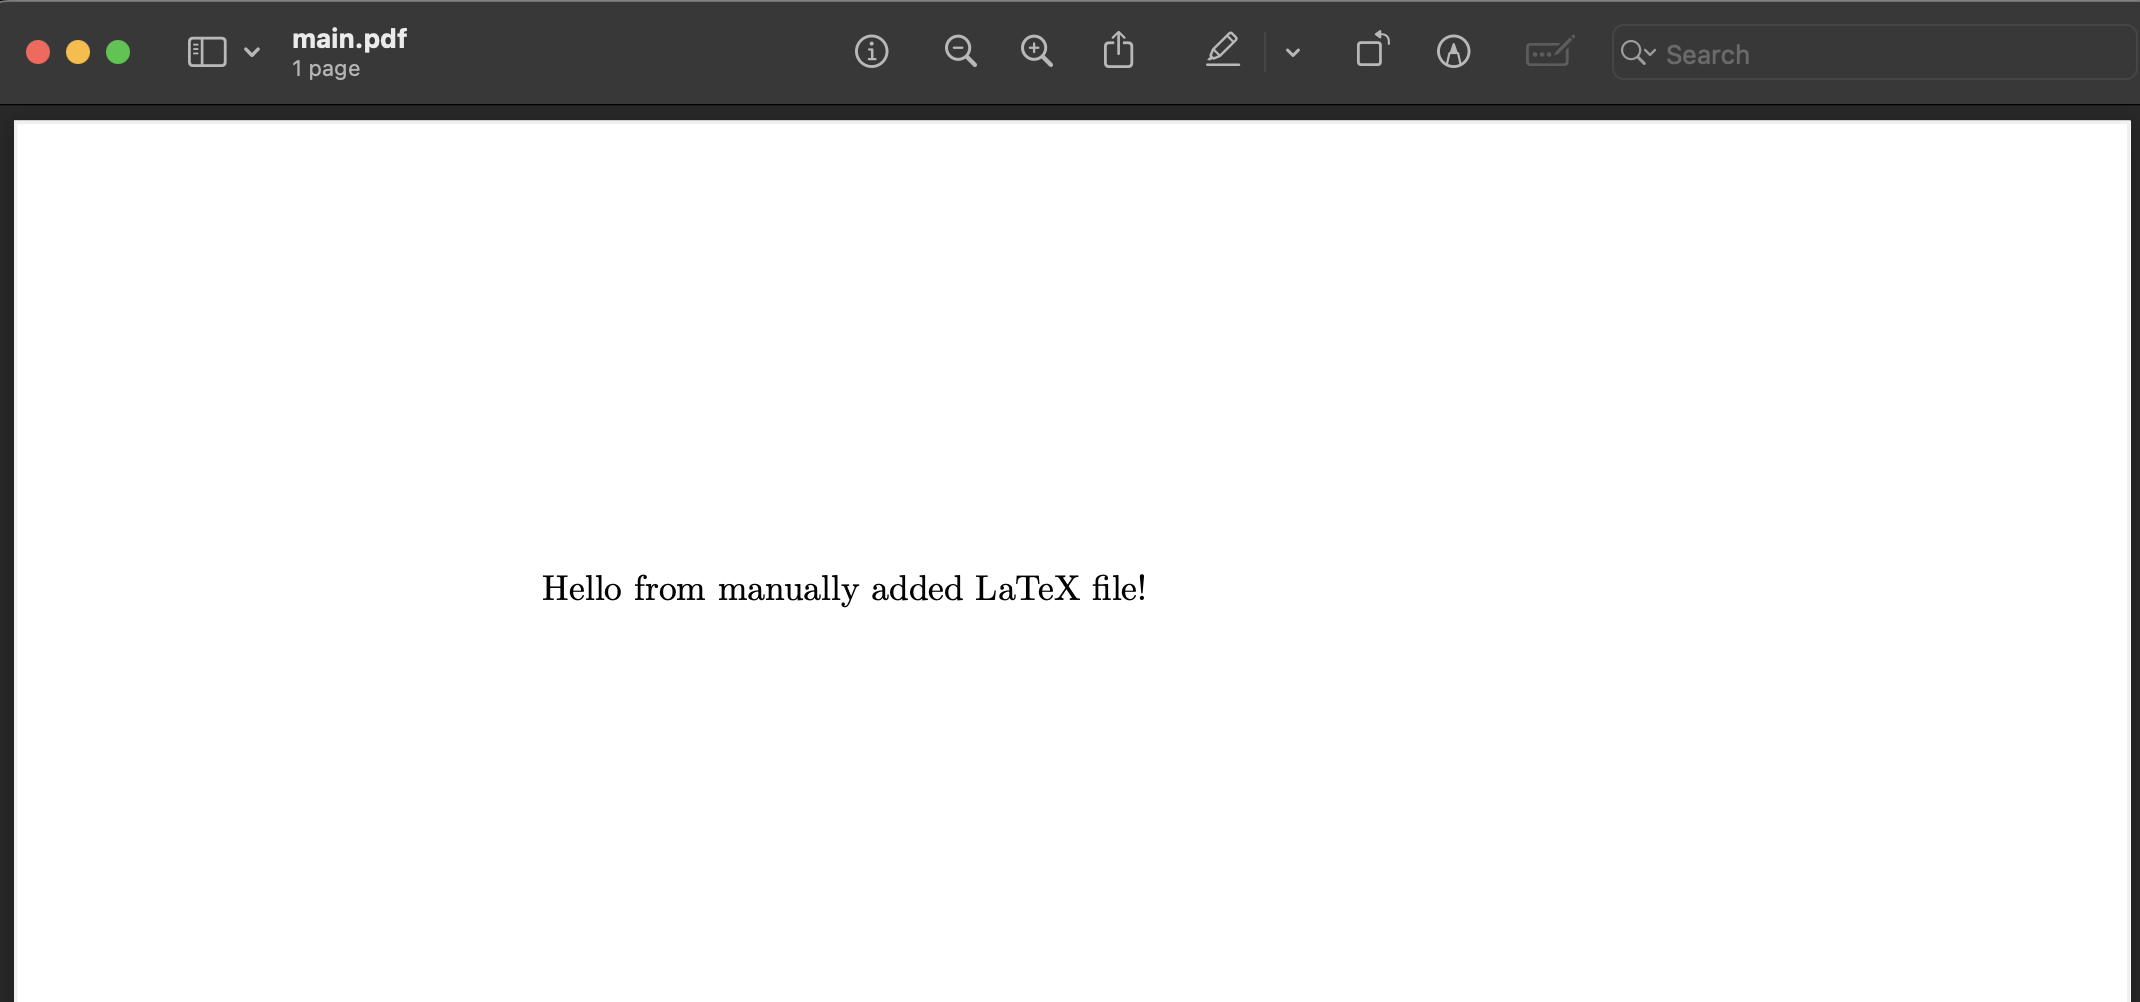
\includegraphics[width=15cm, height=10cm]{png/docker/docker_latex.png}
    \caption{Docker compiled LaTeX document}
    \label{fig:Part I LaTeX}
\end{figure}

\chapter[Bugzilla]{Bugzilla \\\small{\textit{-- Charles, Justin, Benedict, Jacky}}}
\label{Chapter::Bugzilla}
\index{Chapter!Bugzilla}

\begin{enumerate}
    \item Setup Cloud Infrastructure and Access
    \begin{itemize}
        \item Created a Digital Ocean account and created a Ubuntu Droplet VM.
        \item Secured access by generating and adding an SSH key to the Droplet.
    \end{itemize}
    
    \item Prepare Container Environment
    \begin{itemize}
        \item Cloned the Bugzilla source code.
        \item Installed and fixed the missing dependencies (Docker Compose and the Docker service daemon) needed to run containers.
    \end{itemize}
    
    \item Deploy Application Containers
    \begin{itemize}
        \item Used Docker Compose to launch two linked services: the Bugzilla web application container and the MariaDB database container.
        \item Ensured the application's internal network port was mapped to the Droplet's external port 8080.
    \end{itemize}
    
    \item Finalize Configuration
    \begin{itemize}
        \item Executed the required Bugzilla setup script (checksetup.pl) inside the running web container to build the database schema and verify system readiness.
    \end{itemize}
    
    \item Access and Admin Creation
    \begin{itemize}
        \item Confirmed the application was accessible in a web browser at the public IP and port (http://174.138.69.132.8080).
        \item Completed the final step by creating the administrator account via the web interface.
        \item Deleted the Droplet (which is why the link might not work anymore) to avoid any unnecessary billing.
    \end{itemize}
    
\end{enumerate}

\begin{figure}[htp]
    \centering
    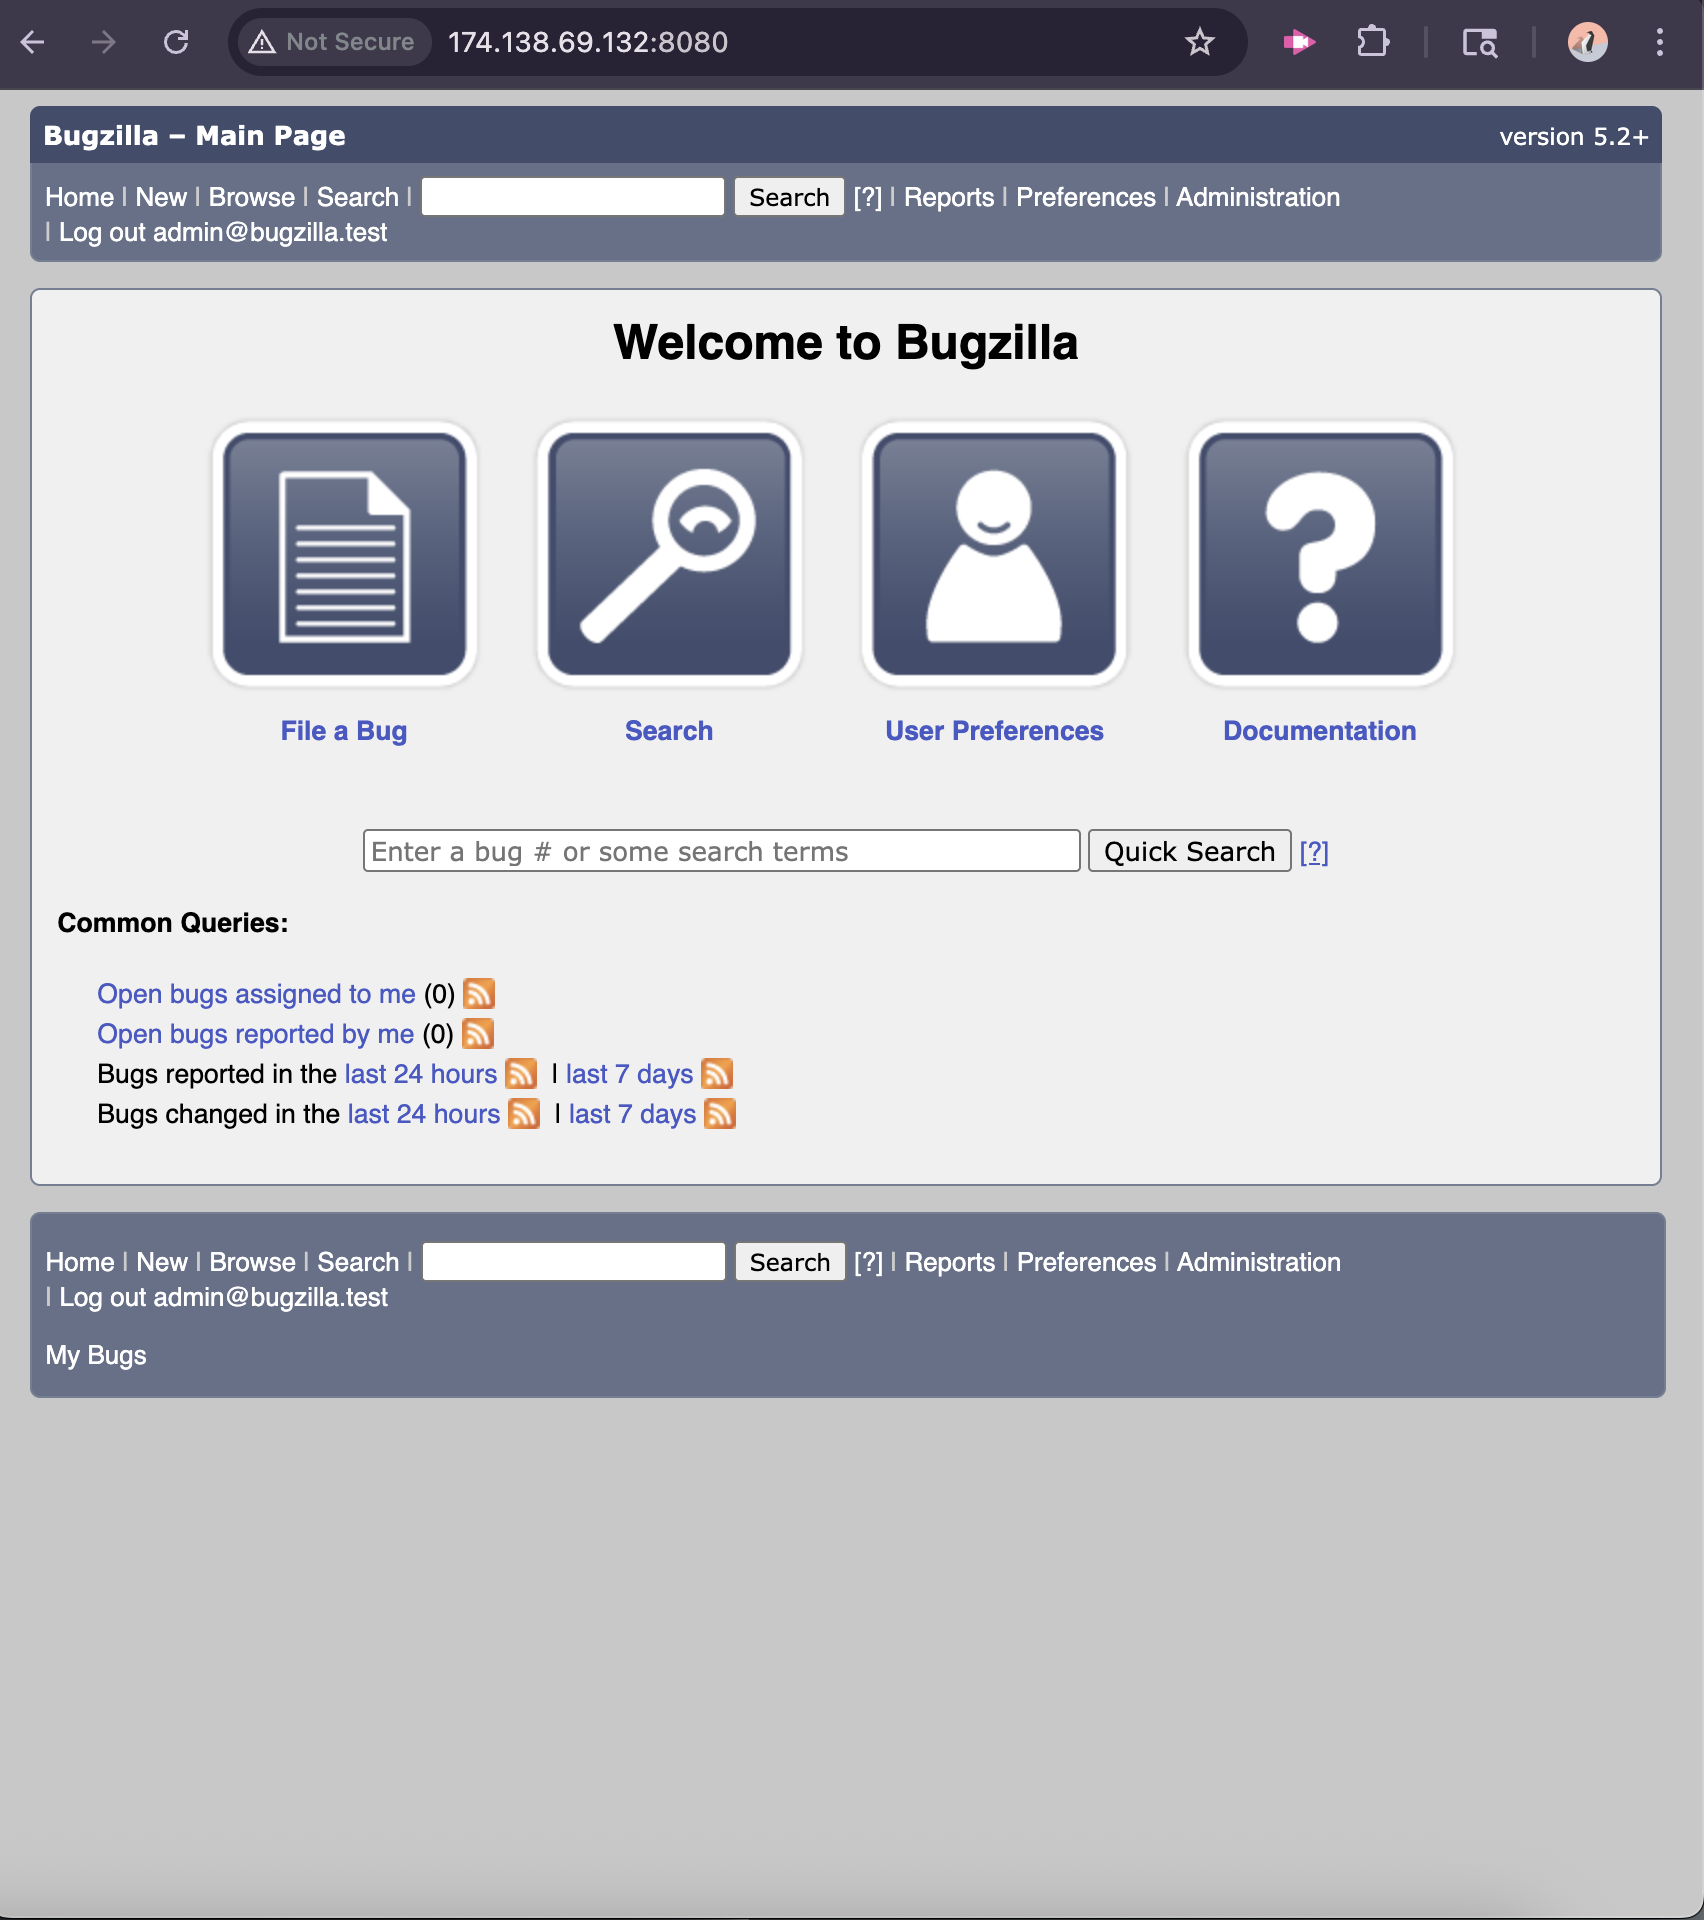
\includegraphics[width=15cm, height=10cm]{png/DigitalOcean/Bugzilla.png}
    \caption{Bugzilla Container Running Screenshot}
    \label{fig:Bugzilla}
\end{figure}
\chapter[Overleaf]{Overleaf \\\small{\textit{-- Charles, Justin, Benedict, Jacky}}}
\label{Chapter::Overleaf}
\index{Chapter!Overleaf}

\begin{enumerate}
    \item Setup Cloud Infrastructure and Access
    \begin{itemize}
        \item Created a Digital Ocean Droplet (VM) running  Ubuntu.
        \item Secured access to the server by using the SSH protocol through the local terminal, which was made in the Bugzilla step.
        \item Resolved an initial SSH access issue to gain root privileges on the Droplet.
    \end{itemize}

    \item Prepare Container Environment
    \begin{itemize}
        \item Installed the necessary container tools (Docker Engine and Docker Compose V1), resolving dependency issues with the correct package name.
        \item Cloned the Overleaf Toolkit source code into the overleaf-ce directory.
        \item Edited the config/overleaf.tc file to set the application's public-facing address and listen on the appropriate IP/Port:
        \begin{itemize}
            \item Set OVERLEAF\_LISTEN\_IP=0.0.0.0 and OVERLEAF\_PORT=80
        \end{itemize}
    \end{itemize}

    \item Deploy Application Containers
    \begin{itemize}
        \item Launched the linked services (sharelatex, mongo, and redis) using the Toolkit's wrapper script "bin/up -d".
        \item Configured the host firewall (UFW) to allow external HTTP traffic on Port 80, exposing the application to the public internet.
    \end{itemize}

    \item Access and Admin Creation
    \begin{itemize}
        \item Confirmed the application was accessible in a web browser at the public IP and port (http://104.236.74.225).
        \item Deleted the Droplet (which is why the link might not work anymore) to avoid any unnecessary billing.
    \end{itemize}
\end{enumerate}

\begin{figure}[htp]
    \centering
    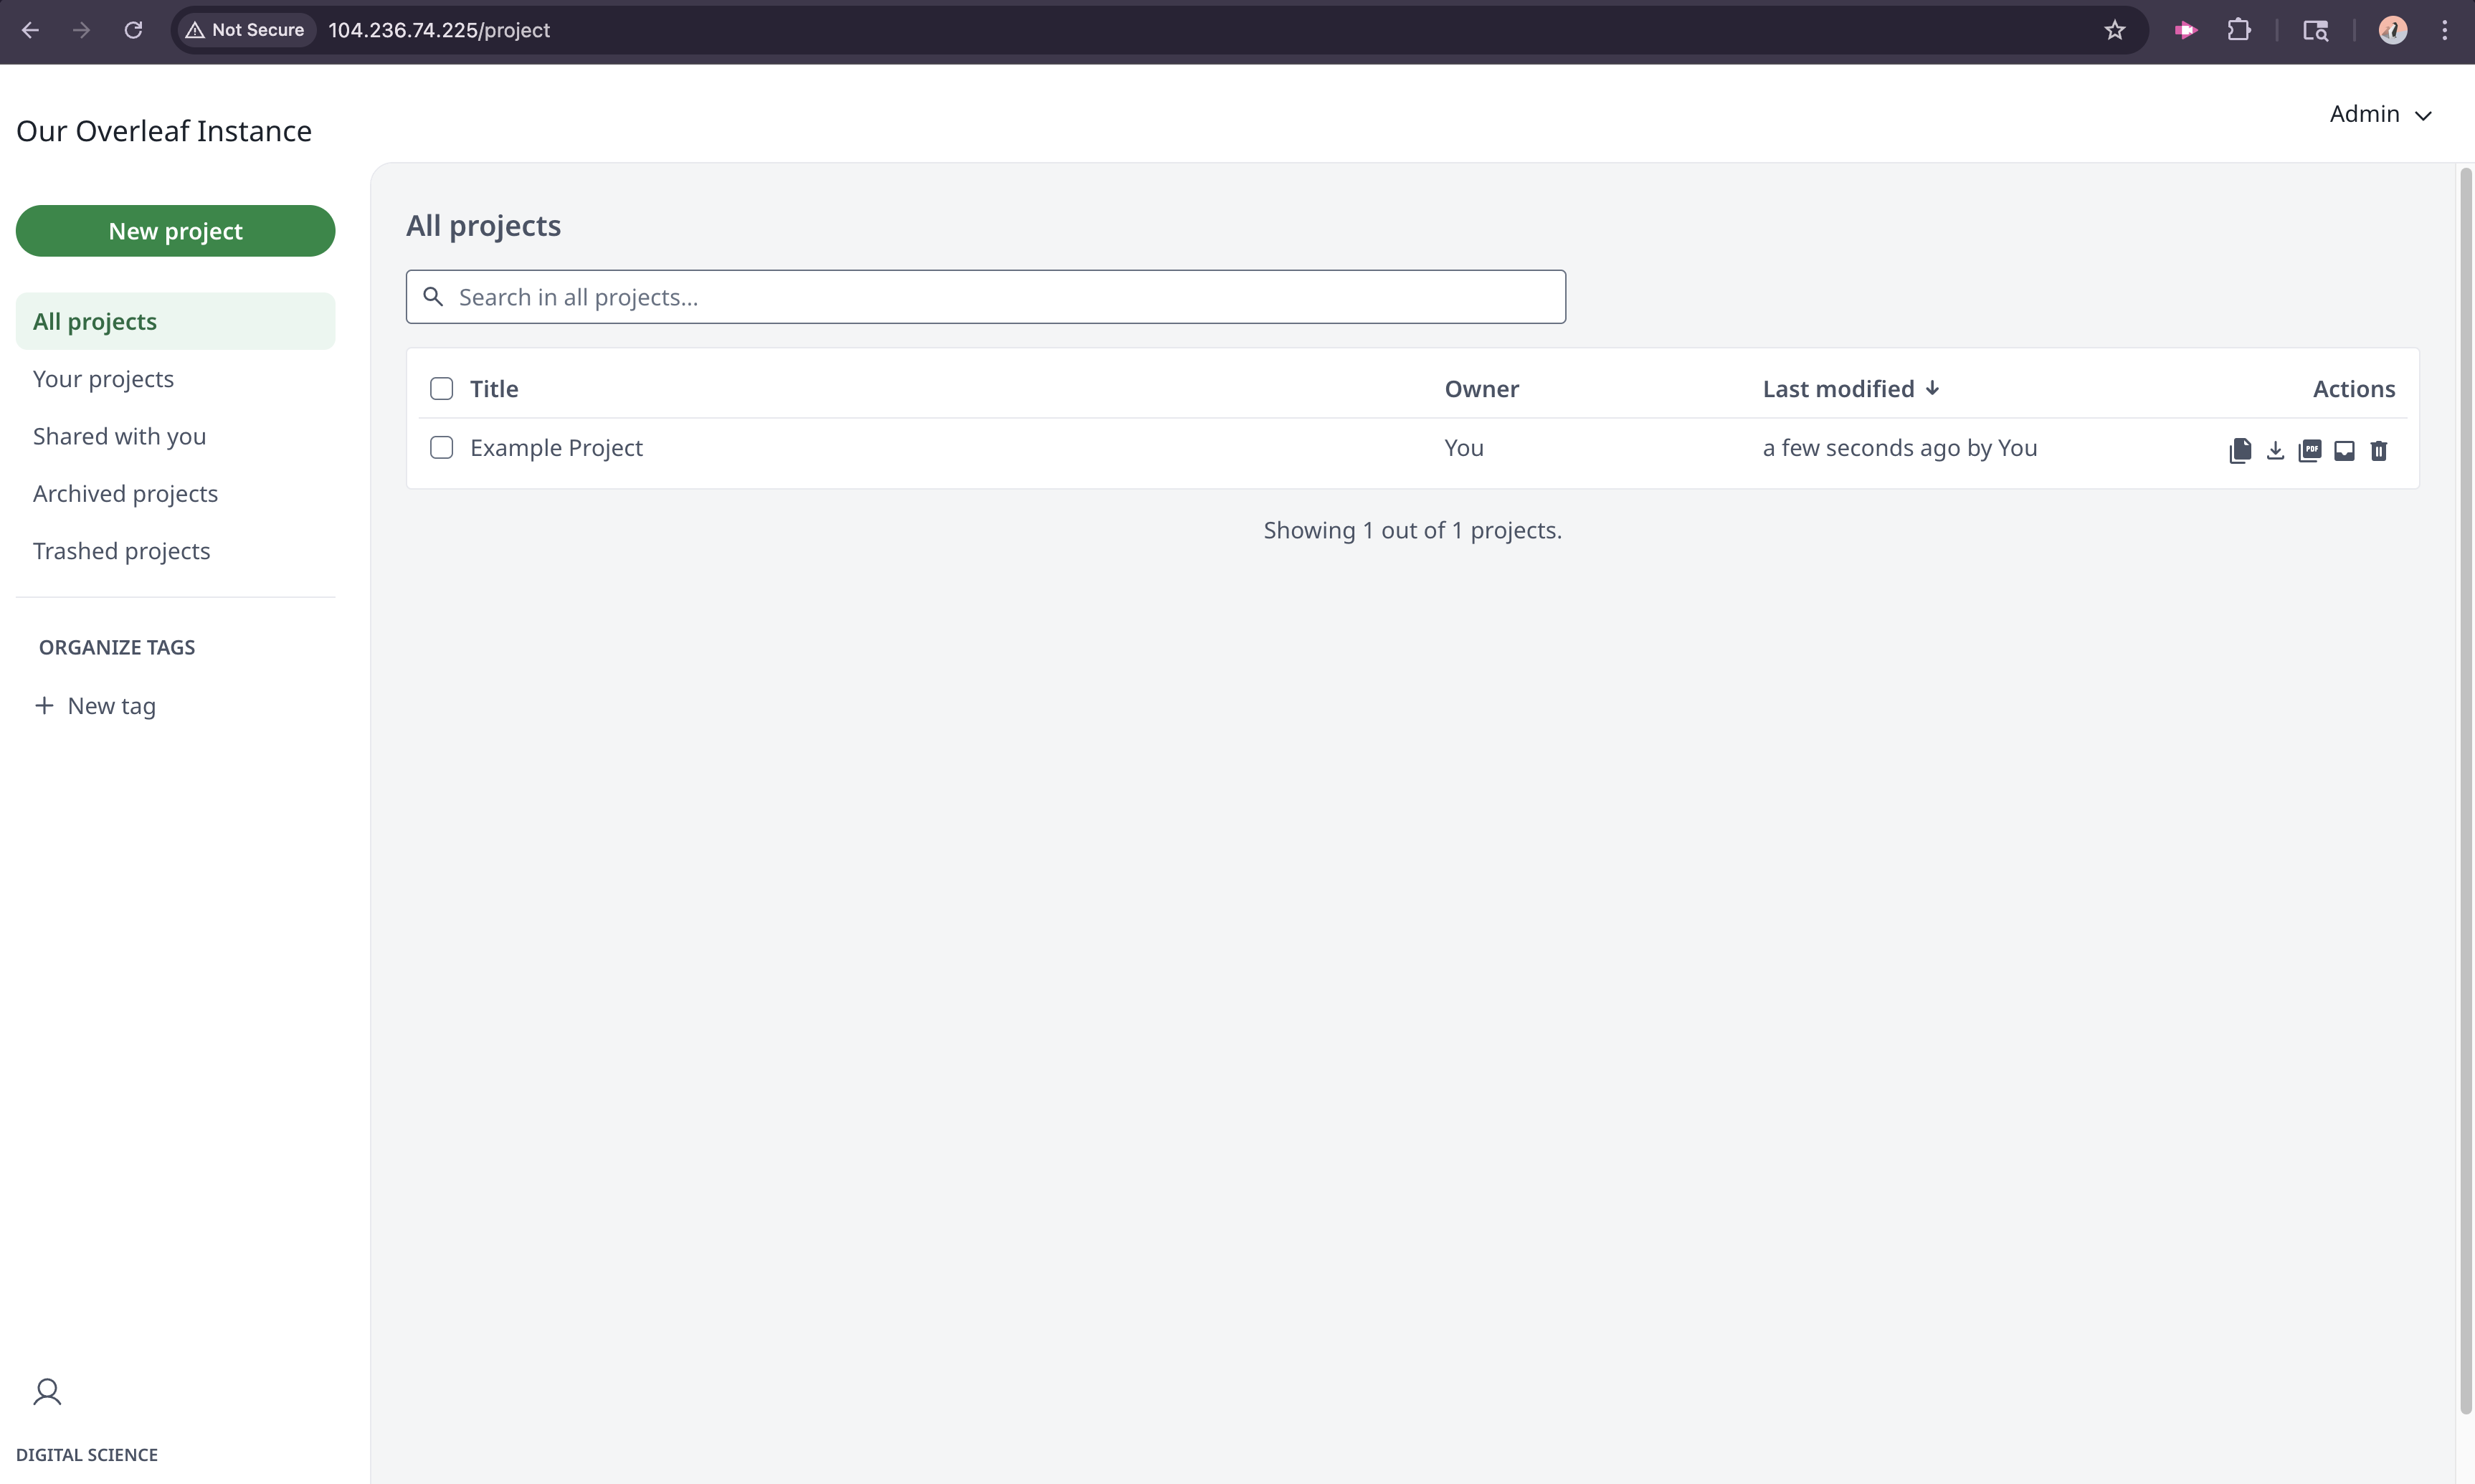
\includegraphics[width=15cm, height=10cm]{png/DigitalOcean/OverleafInstanceMainMenu.png}
    \caption{Overleaf Instance Main Menu Screenshot}
    \label{fig:OverleafInstanceMainMenu}
\end{figure}

\begin{figure}[htp]
    \centering
    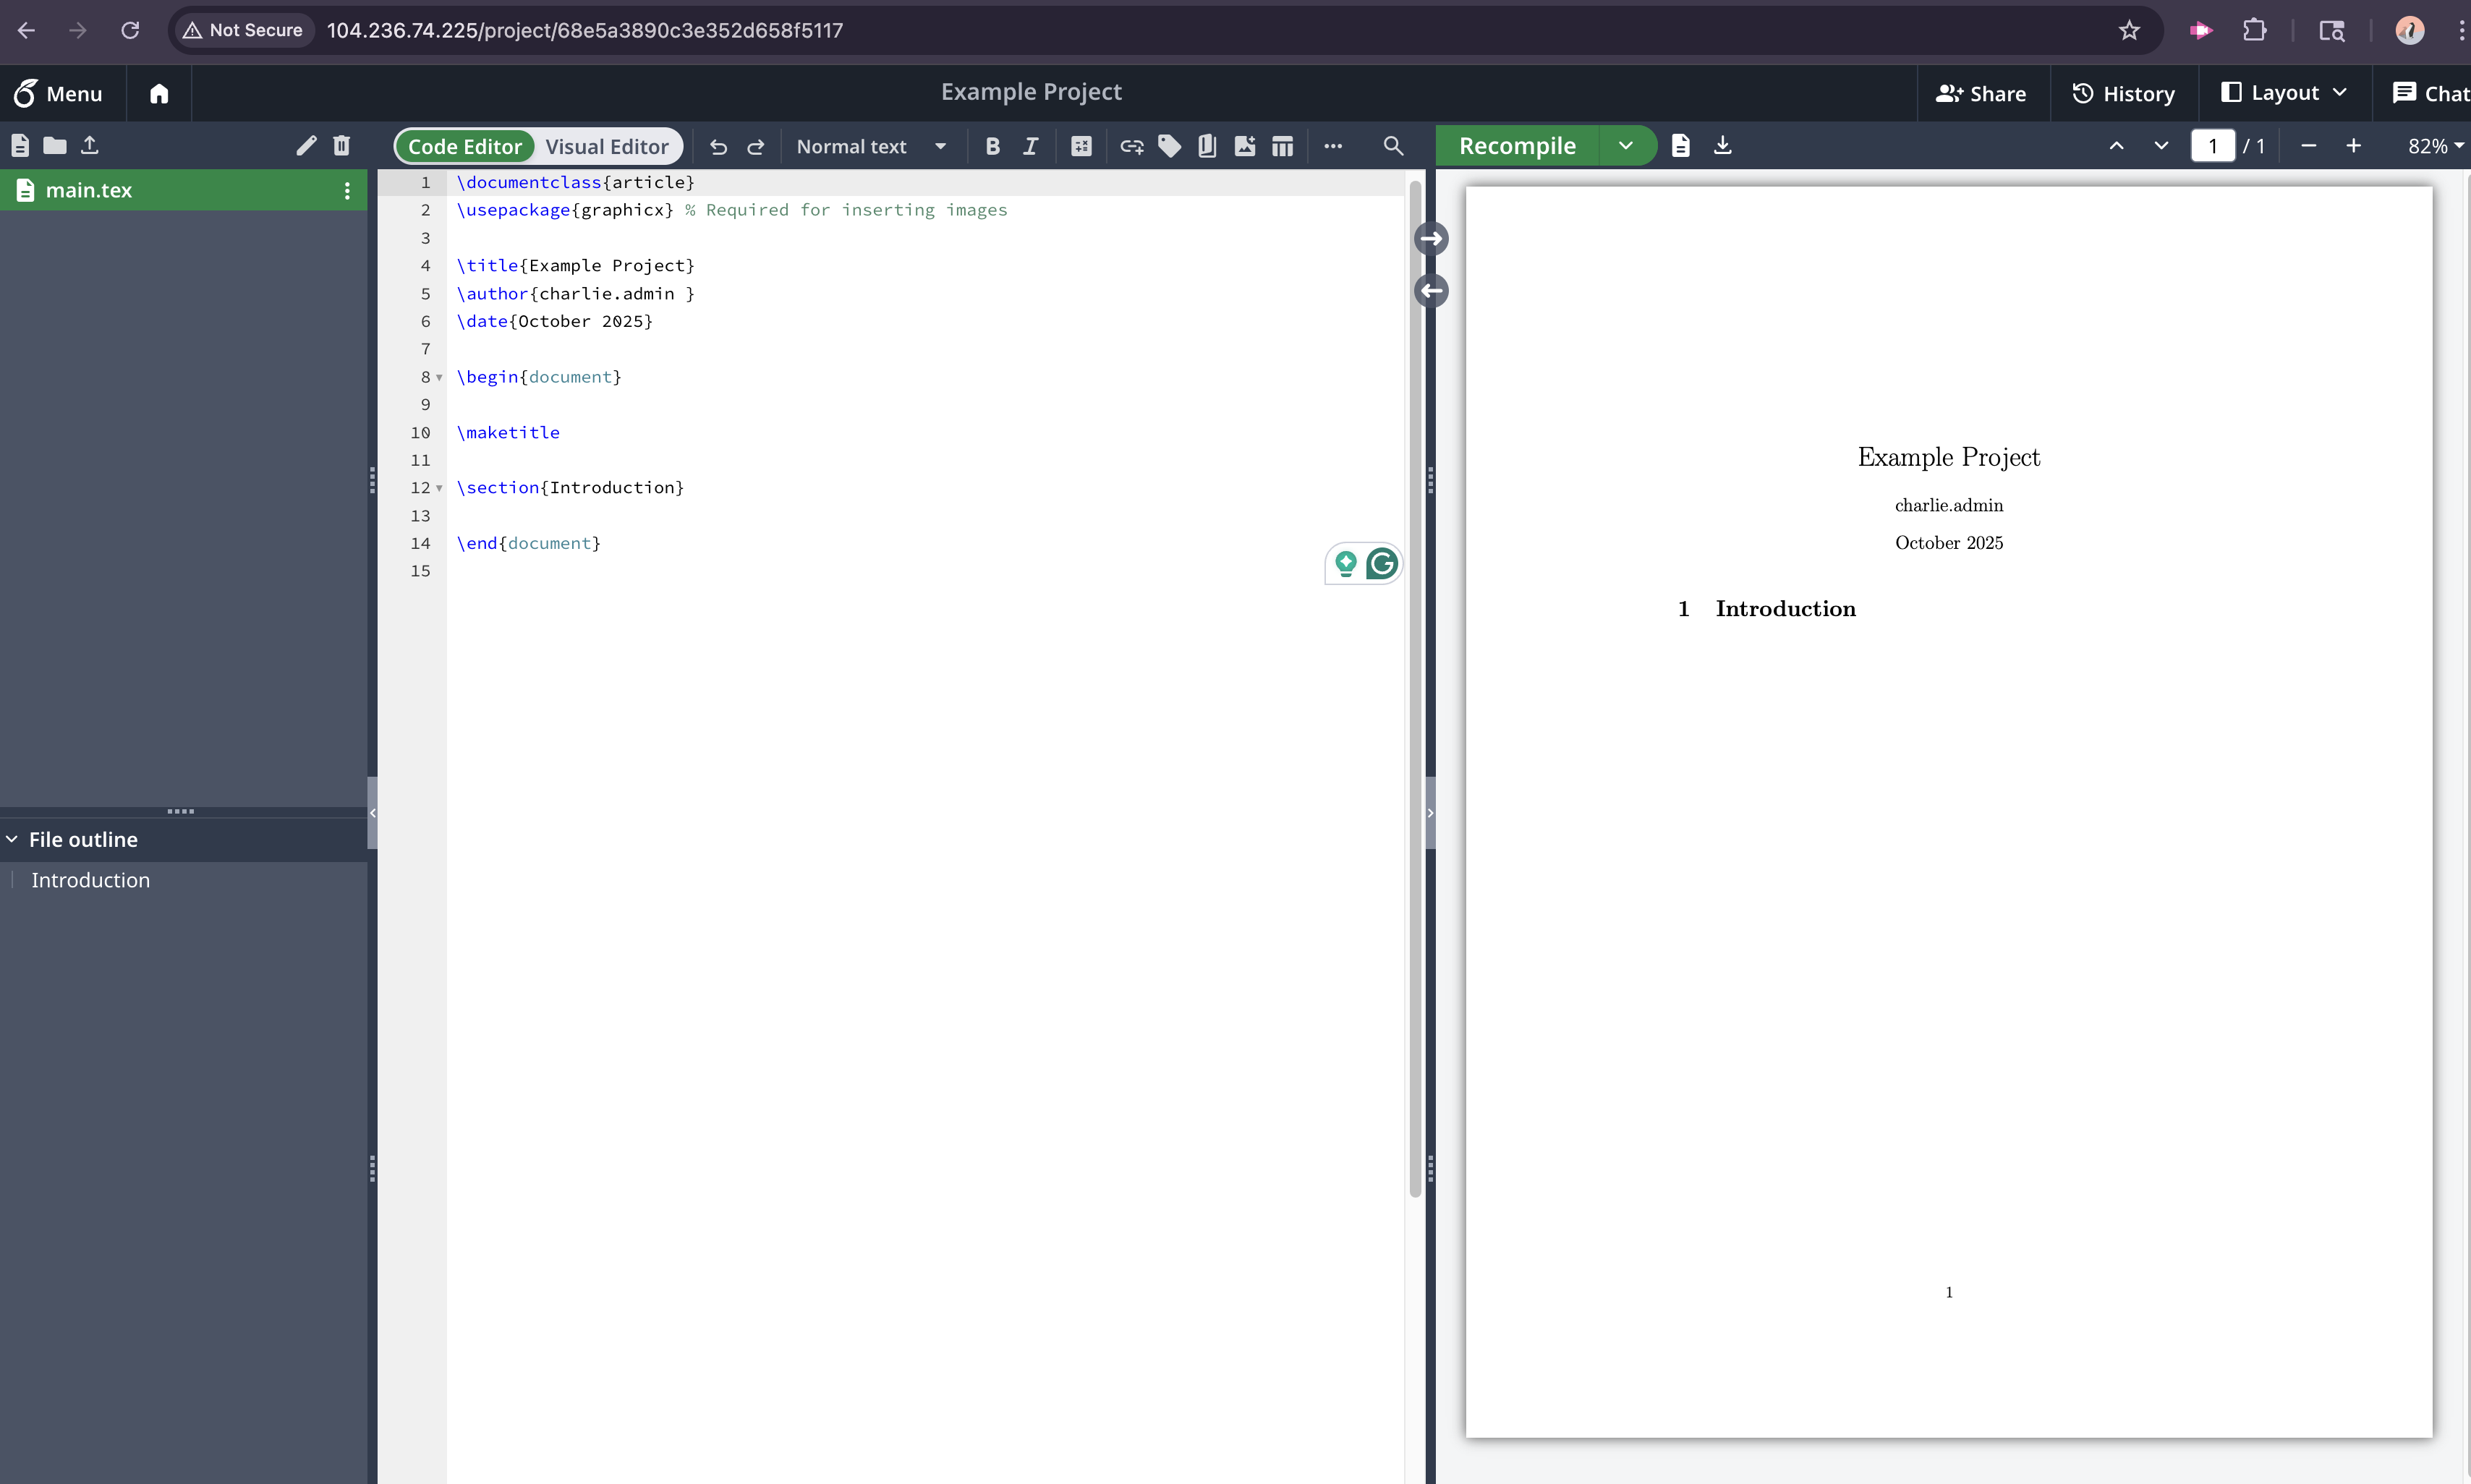
\includegraphics[width=15cm, height=10cm]{png/DigitalOcean/OverleafInstanceExProject.png}
    \caption{Overleaf Instance Example Project Screenshot}
    \label{fig:OverleafInstanceExProject}
\end{figure}
% !TEX program = pdflatex
\chapter[Domain Names]{Domain Names, SSL, and Versioning\\\small{\textit{-- Charles, Justin, Benedict, Jacky}}}
\label{Chapter::Domain Names}
\index{Chapter!Domain Names}

\section{Assignment Overview}
This chapter documents how our group configured a custom domain, secured it with SSL, and connected it to an Overleaf instance hosted via DigitalOcean and GitHub Pages.  
The work combines the DigitalOcean setup (completed by team members on macOS) with my GitHub Pages + SSL configuration.  
Screenshots and command examples are provided for each major step.

%----------------------------------------------------
\section{Step 1: Domain Registration}
Our team registered the domain \textbf{rymarmar.me} using Namecheap through the GitHub Student Developer Pack (free for one year).  
The domain was verified, includes WHOIS privacy protection, and is configured to auto-renew.

\begin{figure}[h!]
    \centering
    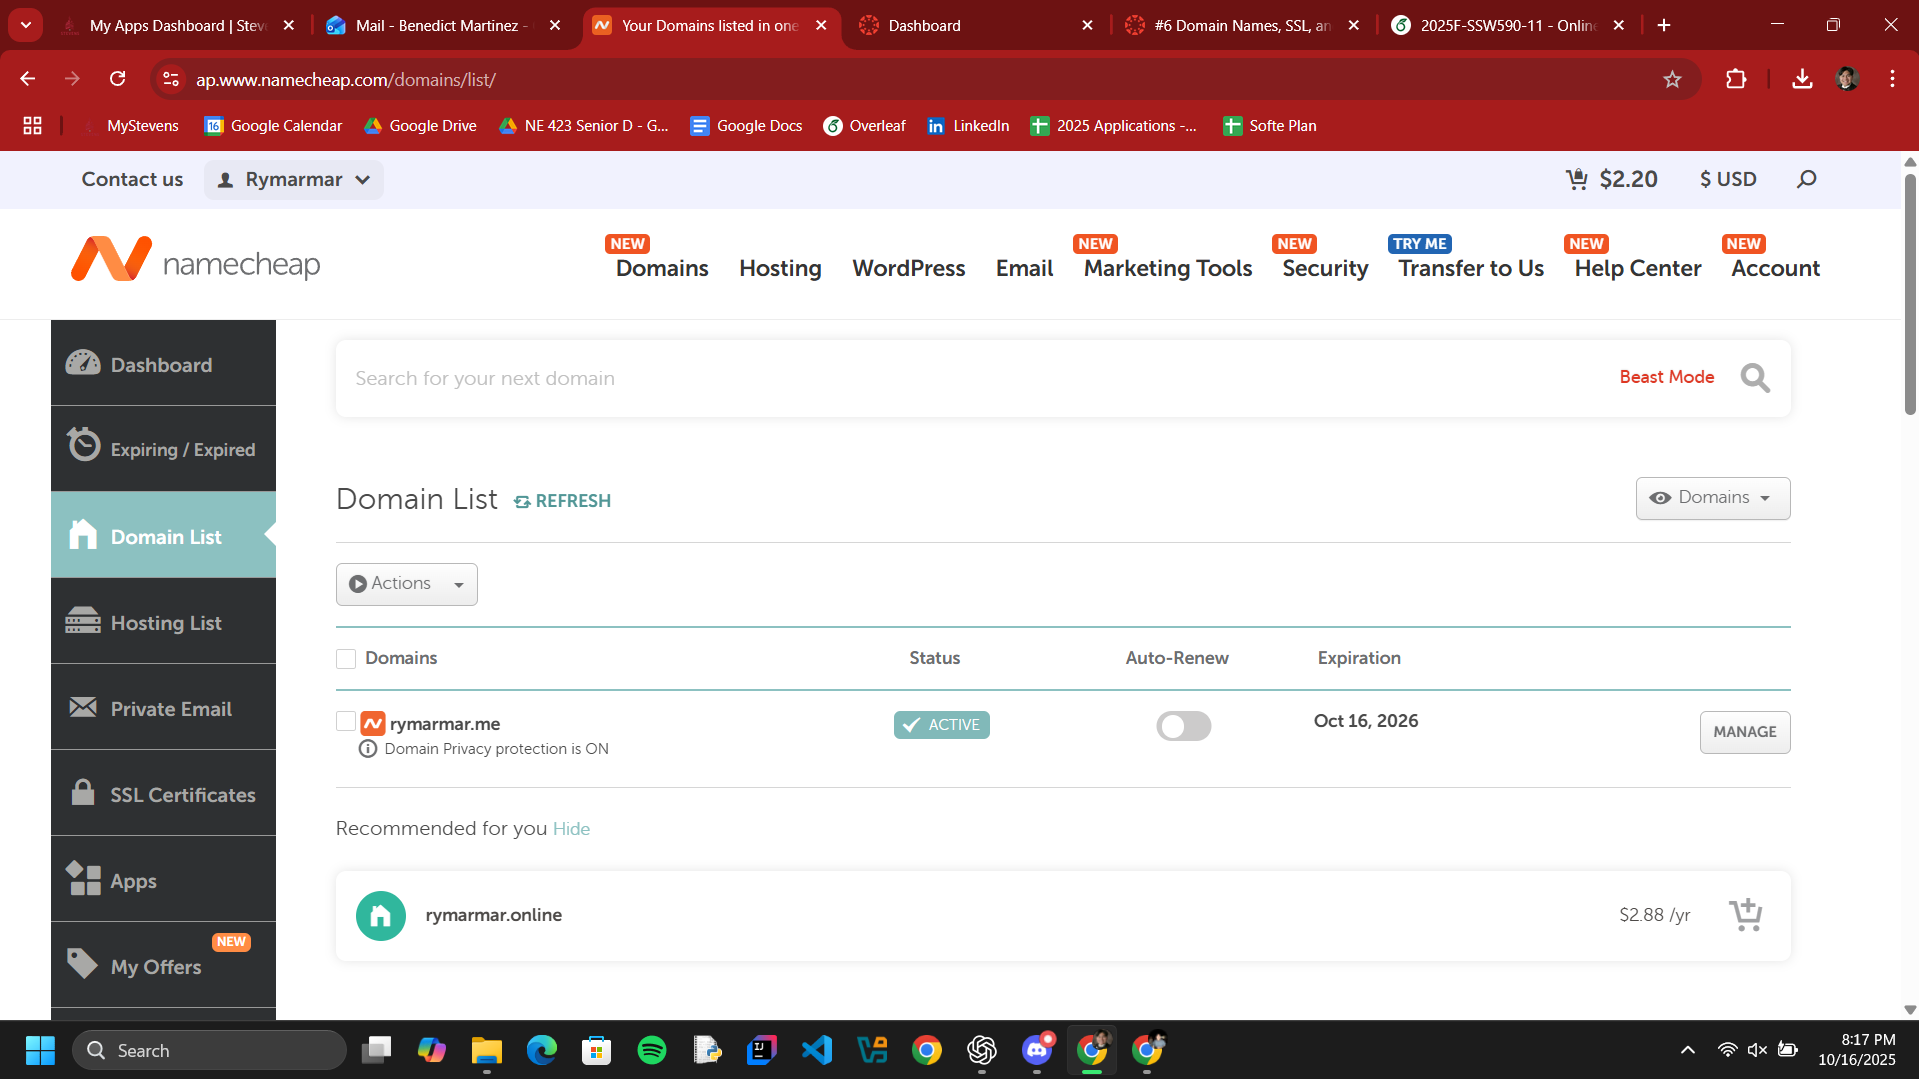
\includegraphics[width=\textwidth]{png/DomainNames/domain_list.png}
    \caption{Namecheap domain list confirming registration of \texttt{rymarmar.me}.}
\end{figure}

%----------------------------------------------------
\section{Step 2: SSL Certificate Configuration}
To secure all traffic, we enabled \textbf{HTTPS enforcement} using GitHub Pages, which automatically provisions SSL certificates through Let’s Encrypt (renewed every 90 days).  
This provides secure HTTPS access without needing to manually install certificates.

\begin{figure}[H]
    \centering
    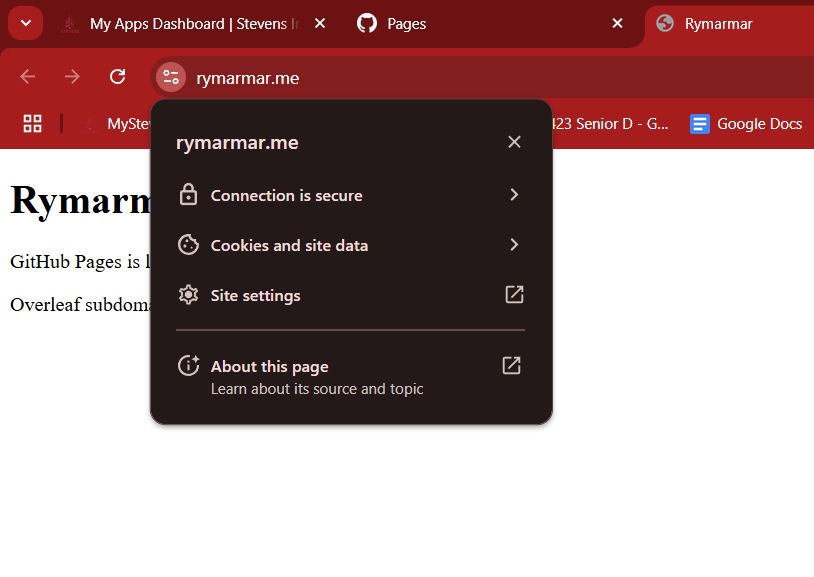
\includegraphics[width=\textwidth]{png/DomainNames/Enforce_HTTPS.png}
    \caption{GitHub Pages settings showing HTTPS enforcement and DNS verification.}
\end{figure}

\begin{figure}[H]
    \centering
    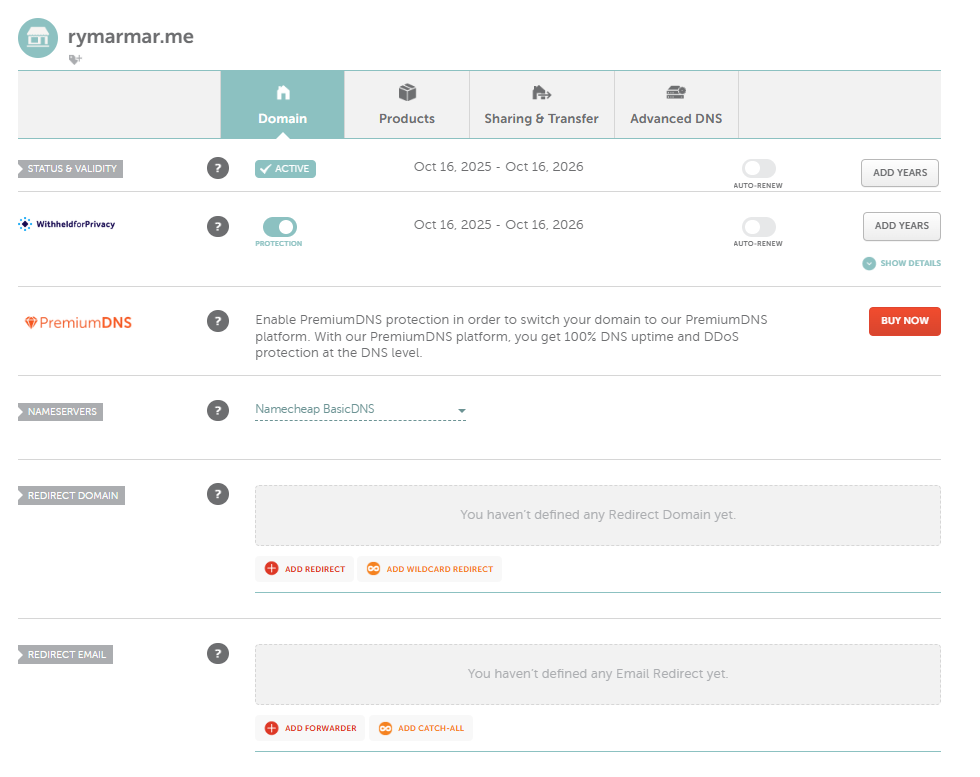
\includegraphics[width=0.7\textwidth]{png/DomainNames/domain_secured.png}
    \caption{Browser confirmation that \texttt{https://rymarmar.me} is secured via SSL.}
\end{figure}

\begin{figure}[H]
    \centering
    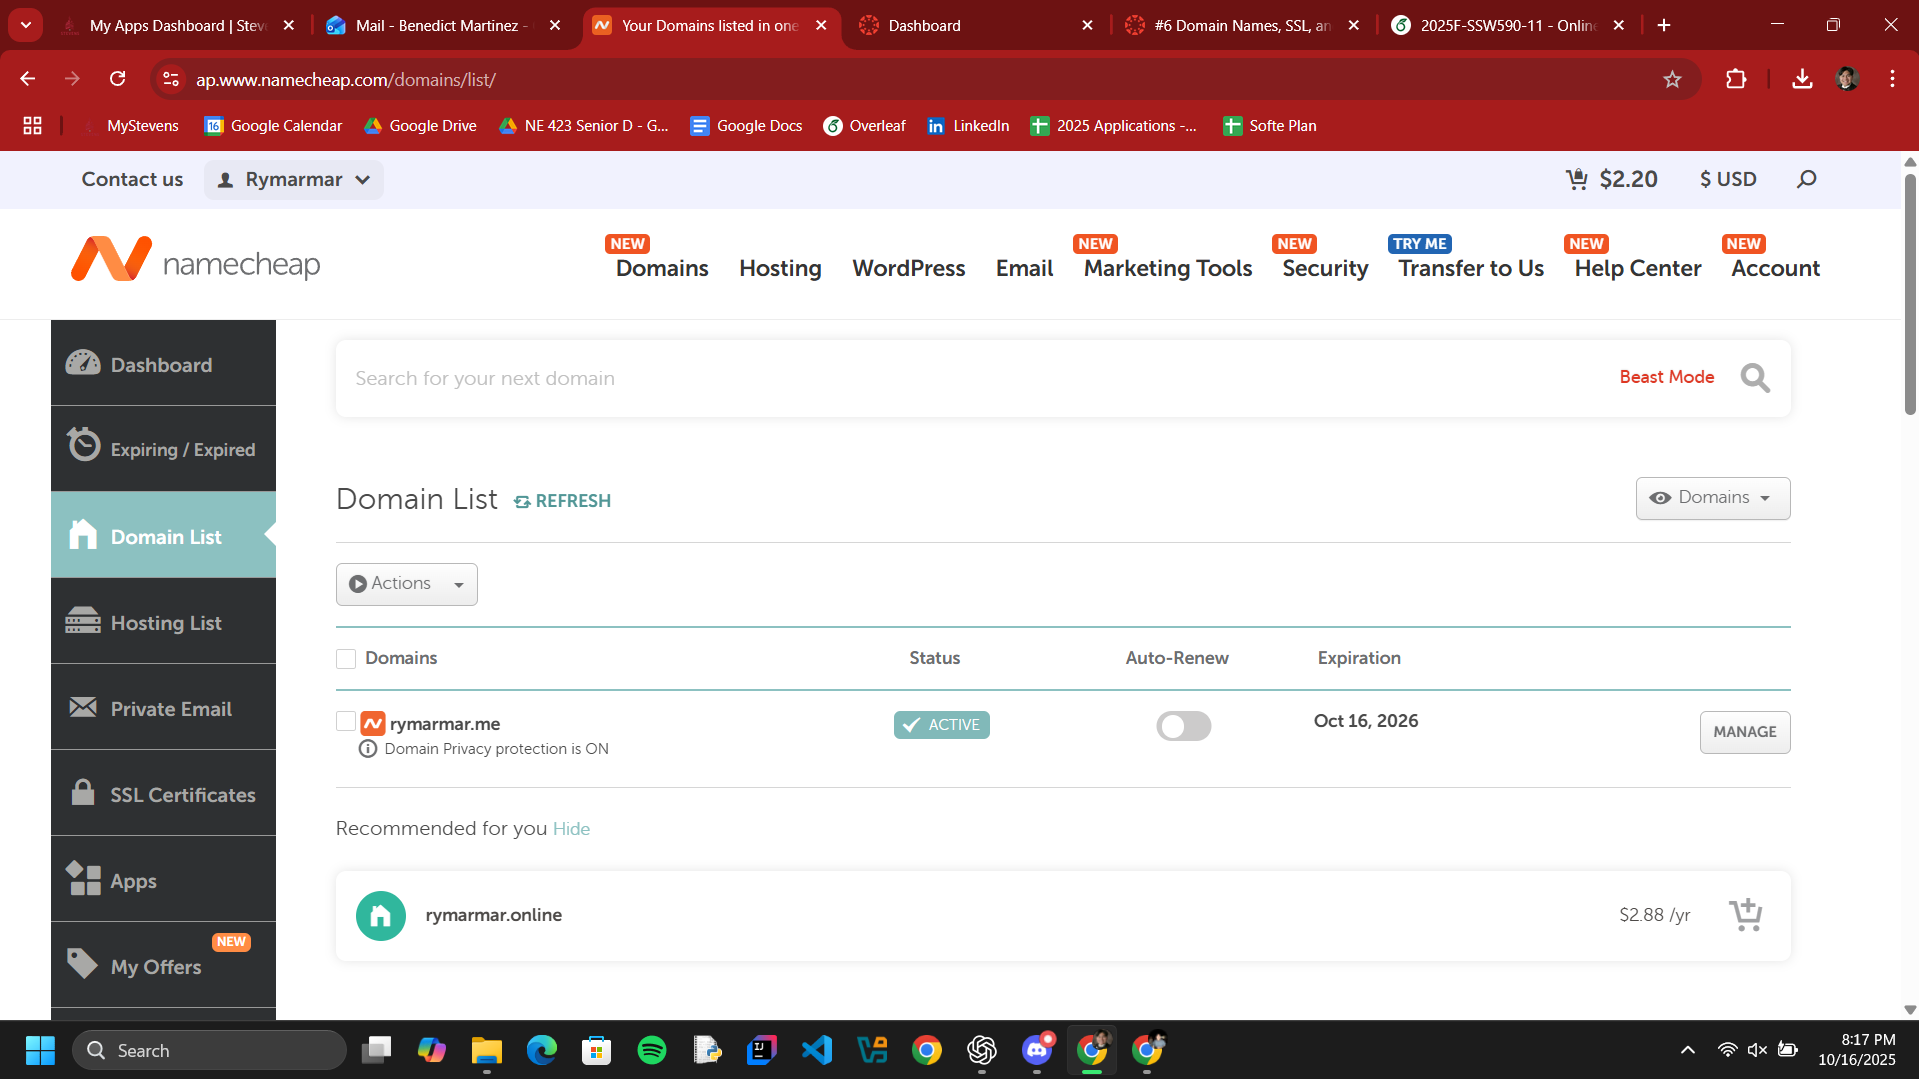
\includegraphics[width=\textwidth]{png/DomainNames/domain_list.png}
    \caption{Namecheap domain list confirming registration of \texttt{rymarmar.me}.}
\end{figure}
%----------------------------------------------------
\section{Step 2.1: SSL Configuration using Caddy}

Another option for providing SSL to the domain is using Caddy. Once installed using apt install caddy, we made a Caddyfile and modified the docker-compose file.    
\begin{figure}[H]
\begin{minted}[linenos]{python}
     1	services:
     2	    sharelatex:
    16	        volumes:
    33	            OVERLEAF_SITE_URL: "https://ssw590team11.me"
   156	    caddy:
   157	      image: caddy:latest
   158	      container_name: caddy
   159	      ports:
   160	        - "80:80"
   161	        - "443:443"
   162	      volumes:
   163	        - ./Caddyfile:/etc/caddy/Caddyfile
   164	        - caddy_data:/data
   165	        - caddy_config:/config
   166	      depends_on:
   167	        - sharelatex
   168	      restart: unless-stopped
   169	volumes:
   170	  mongo_data:
   171	  caddy_data:
   172	  caddy_config:
\end{minted}
\caption{docker-compose.yml additions}
\end{figure}

\begin{figure}[H]
\begin{minted}[linenos]{python}
ssw590team11.me {
	reverse_proxy sharelatex:80
}
\end{minted}
\caption{Caddyfile}
\end{figure}

We also added records on Digital Ocean and Namecheap to link our droplet to the domain.

\begin{figure}[H]
    \centering
    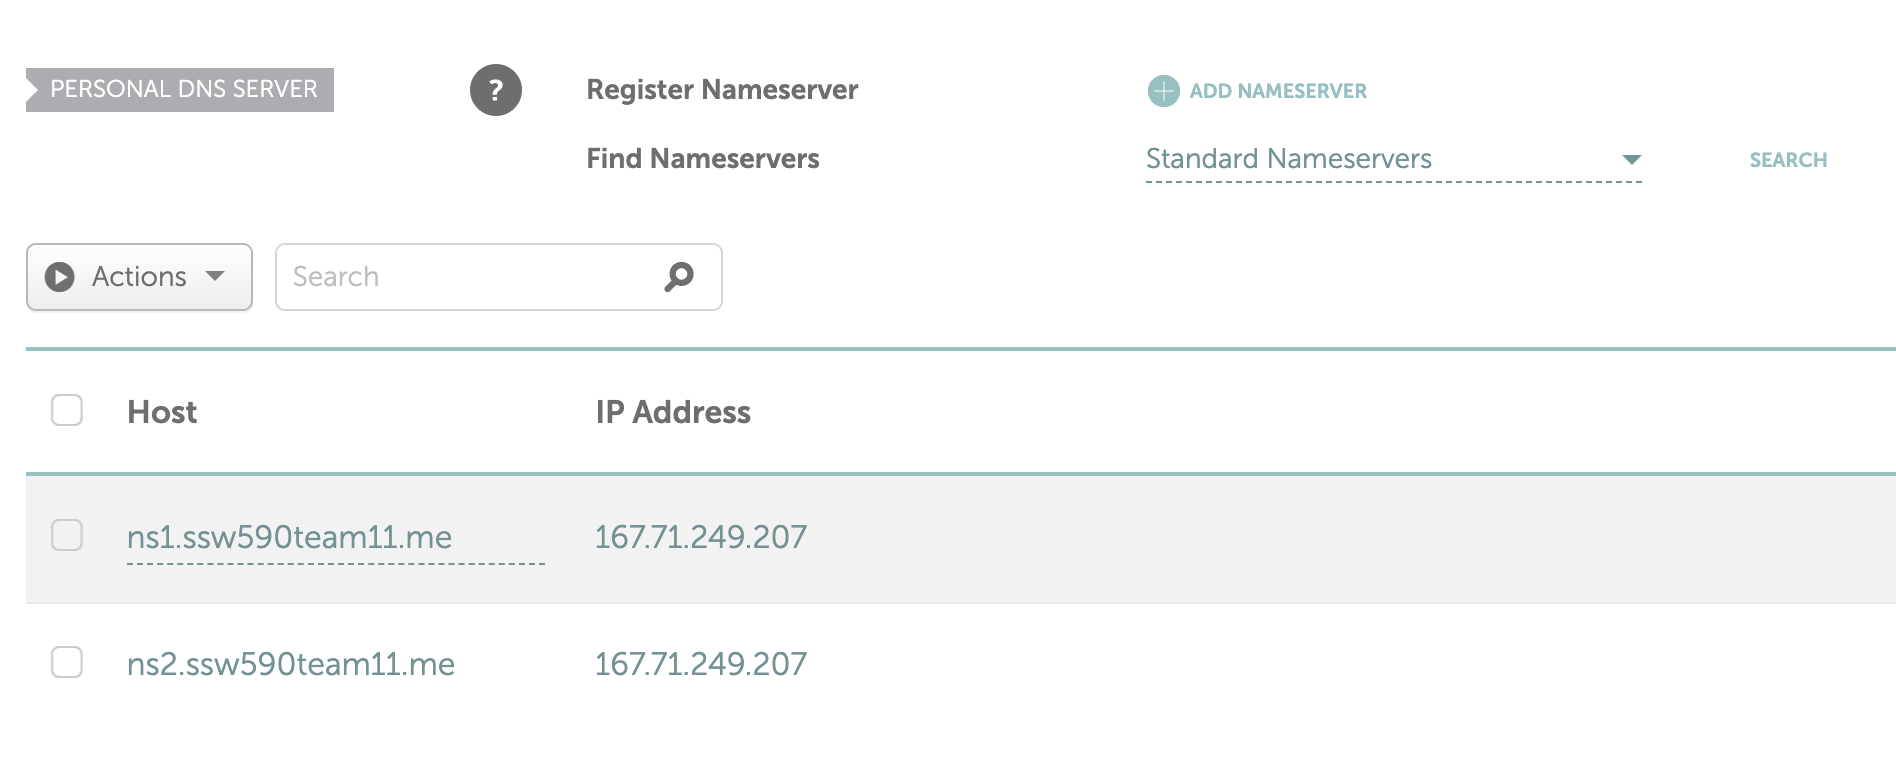
\includegraphics[width=0.7\textwidth]{png/DigitalOcean/DigitalOceanDNS.png}
    \caption{Digital Ocean DNS records linking to domain}
\end{figure}

\begin{figure}[H]
    \centering
    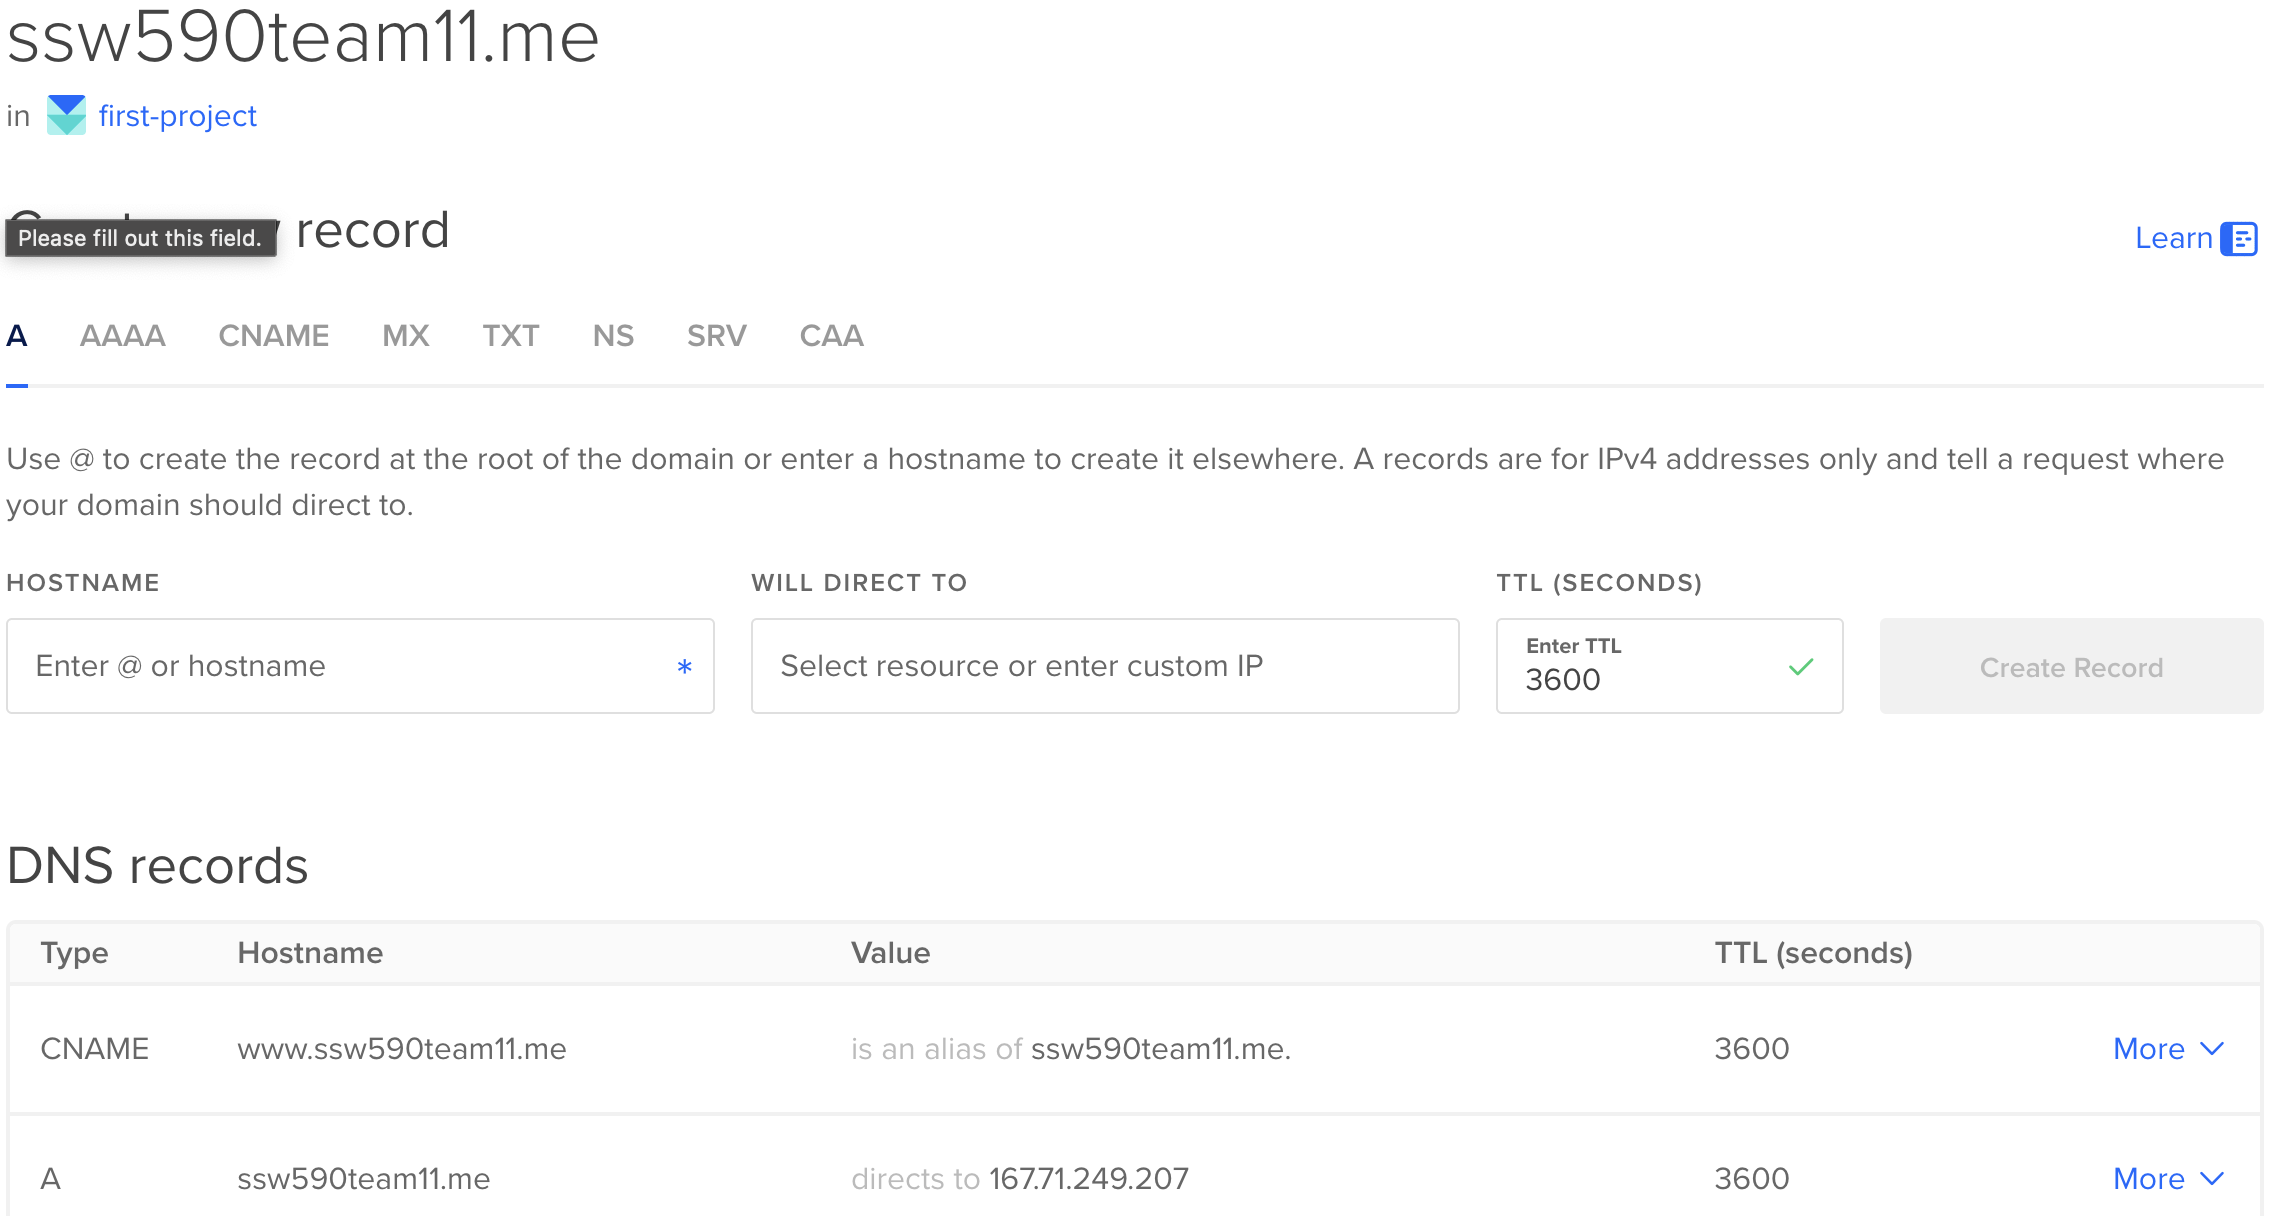
\includegraphics[width=0.7\textwidth]{png/DigitalOcean/NamecheapRecords.png}
    \caption{Namecheap DNS records to go to droplet IP address}
\end{figure}

%----------------------------------------------------
\section{Step 3: Overleaf Container Setup on DigitalOcean}
Our teammates (Charles and Justin) deployed an Overleaf Community Edition container using a DigitalOcean droplet.  
This ensured the Overleaf instance supported all LaTeX packages and allowed testing of compilation consistency.  
The container was connected to our team GitHub repository and included a custom domain mapping for the subdomain.

\begin{minted}{bash}
# Example Docker-based deployment used on DigitalOcean
sudo docker run -d --name overleaf -p 80:80 sharelatex/sharelatex
\end{minted}

This step satisfied the “configure container/image” requirement for Overleaf hosting.  
The configuration process was documented and replicated locally for testing.

\begin{figure}[h!]
    \centering
    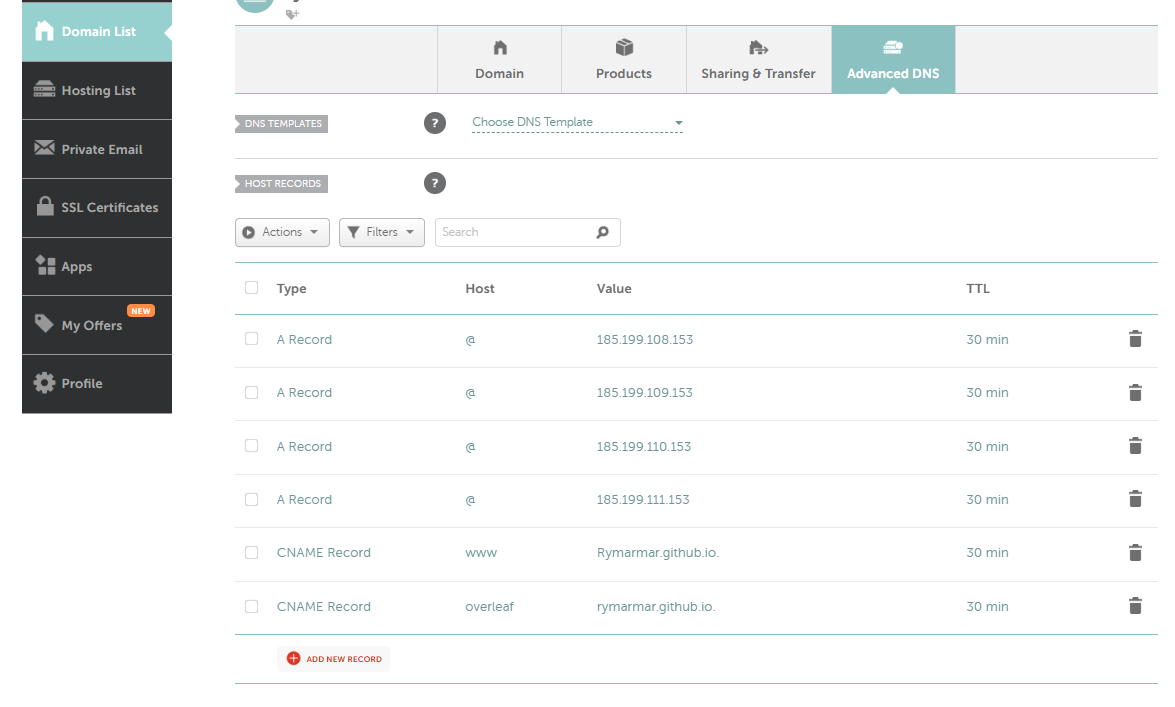
\includegraphics[width=\textwidth]{png/DomainNames/namespacesettings.png}
    \caption{Namecheap Advanced DNS configuration showing A and CNAME records for the root and subdomains.}
\end{figure}

\begin{figure}[h!]
    \centering
    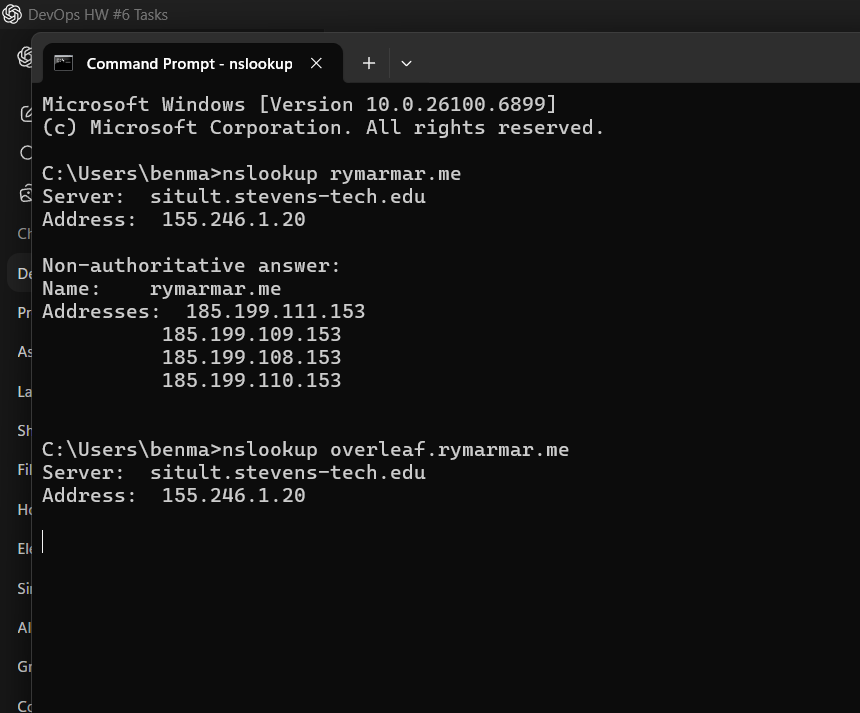
\includegraphics[width=0.85\textwidth]{png/DomainNames/cmd_checkup.png}
    \caption{Verification using \texttt{nslookup} confirming successful DNS and subdomain resolution.}
\end{figure}

%----------------------------------------------------
\section{Step 4: GitHub Pages Integration (Benedict)}
The GitHub repository \texttt{Rymarmar.github.io} was configured to serve as the main site using the custom domain \texttt{rymarmar.me}.  
Deployment is configured directly from the \texttt{main} branch, and HTTPS is now enforced.  
This serves as a simple landing page while the Overleaf container is being finalized.

\begin{figure}[h!]
    \centering
    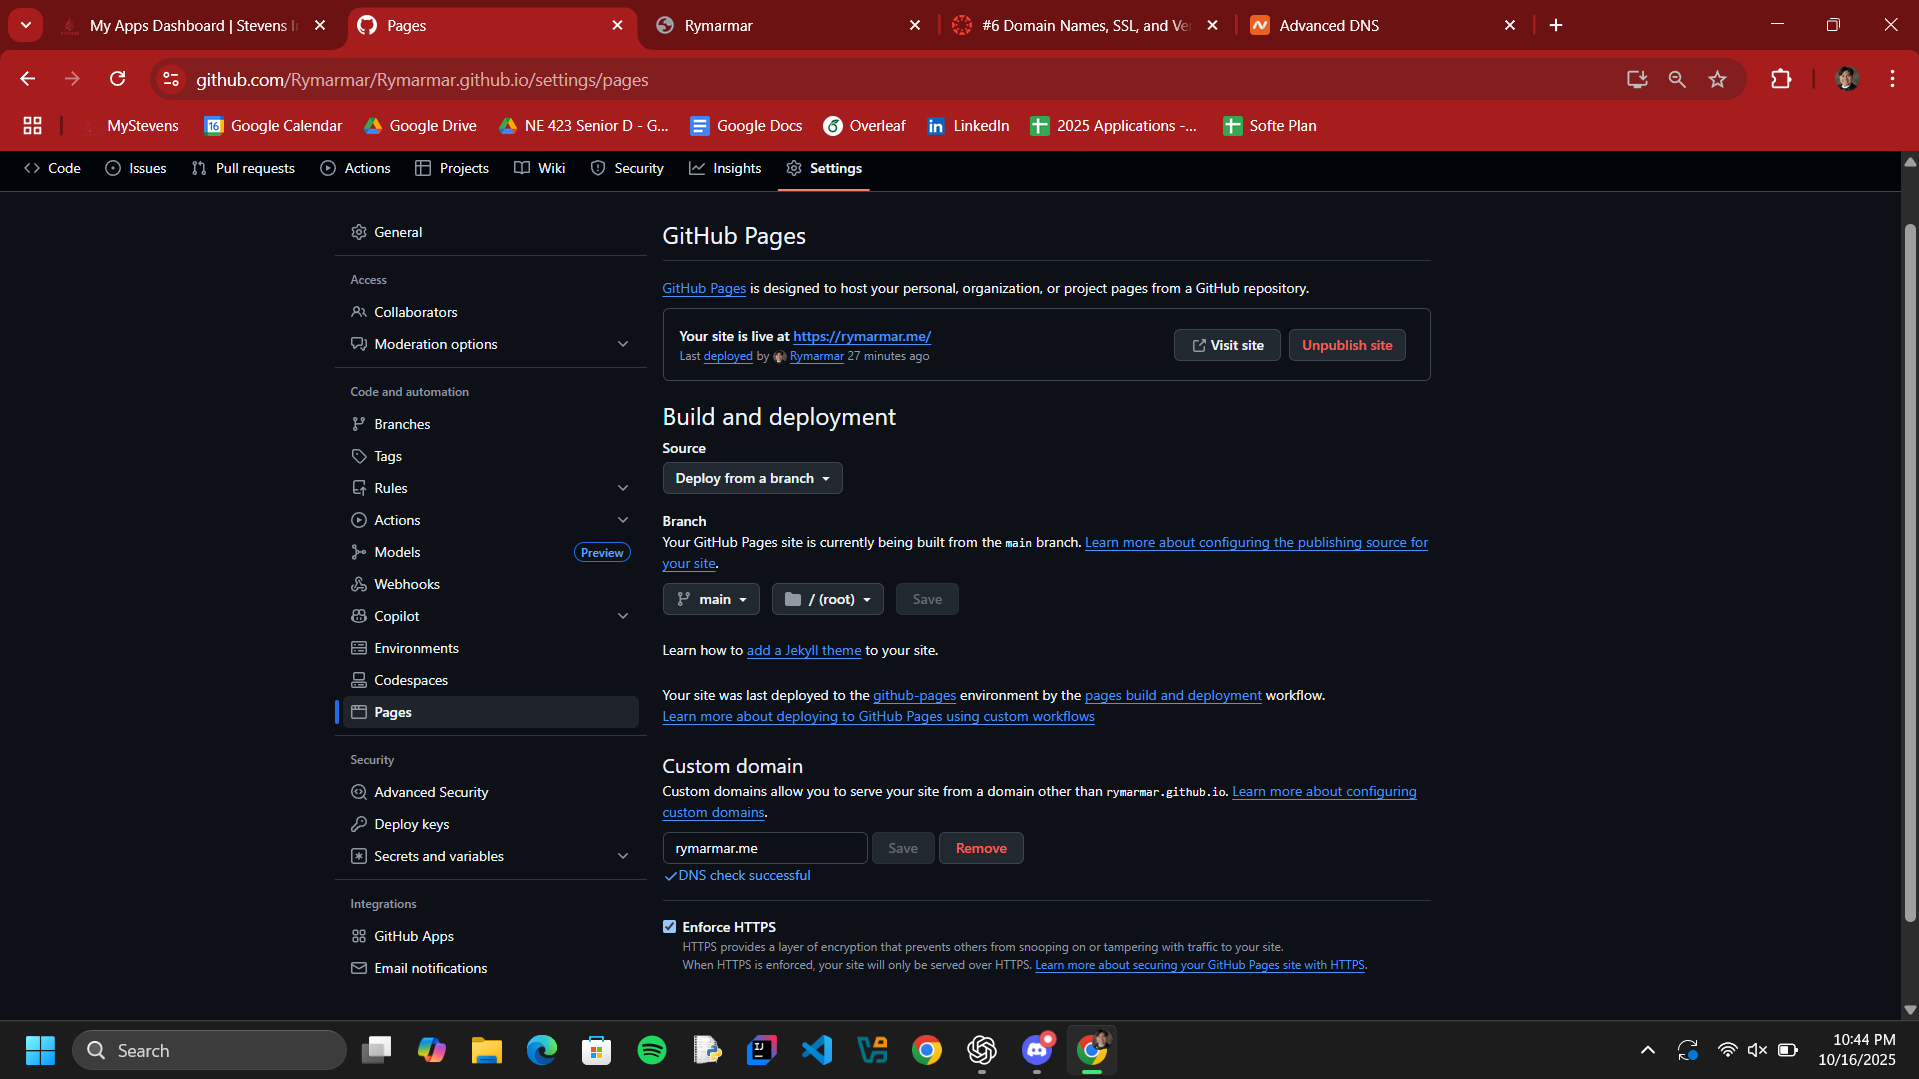
\includegraphics[width=\textwidth]{png/DomainNames/github settings.png}
    \caption{GitHub Pages settings confirming DNS validation and HTTPS enforcement.}
\end{figure}

The \texttt{index.html} page was published successfully. Some users experienced delays when loading the domain due to DNS propagation time, but configuration remains correct.

\begin{figure}[h!]
    \centering
    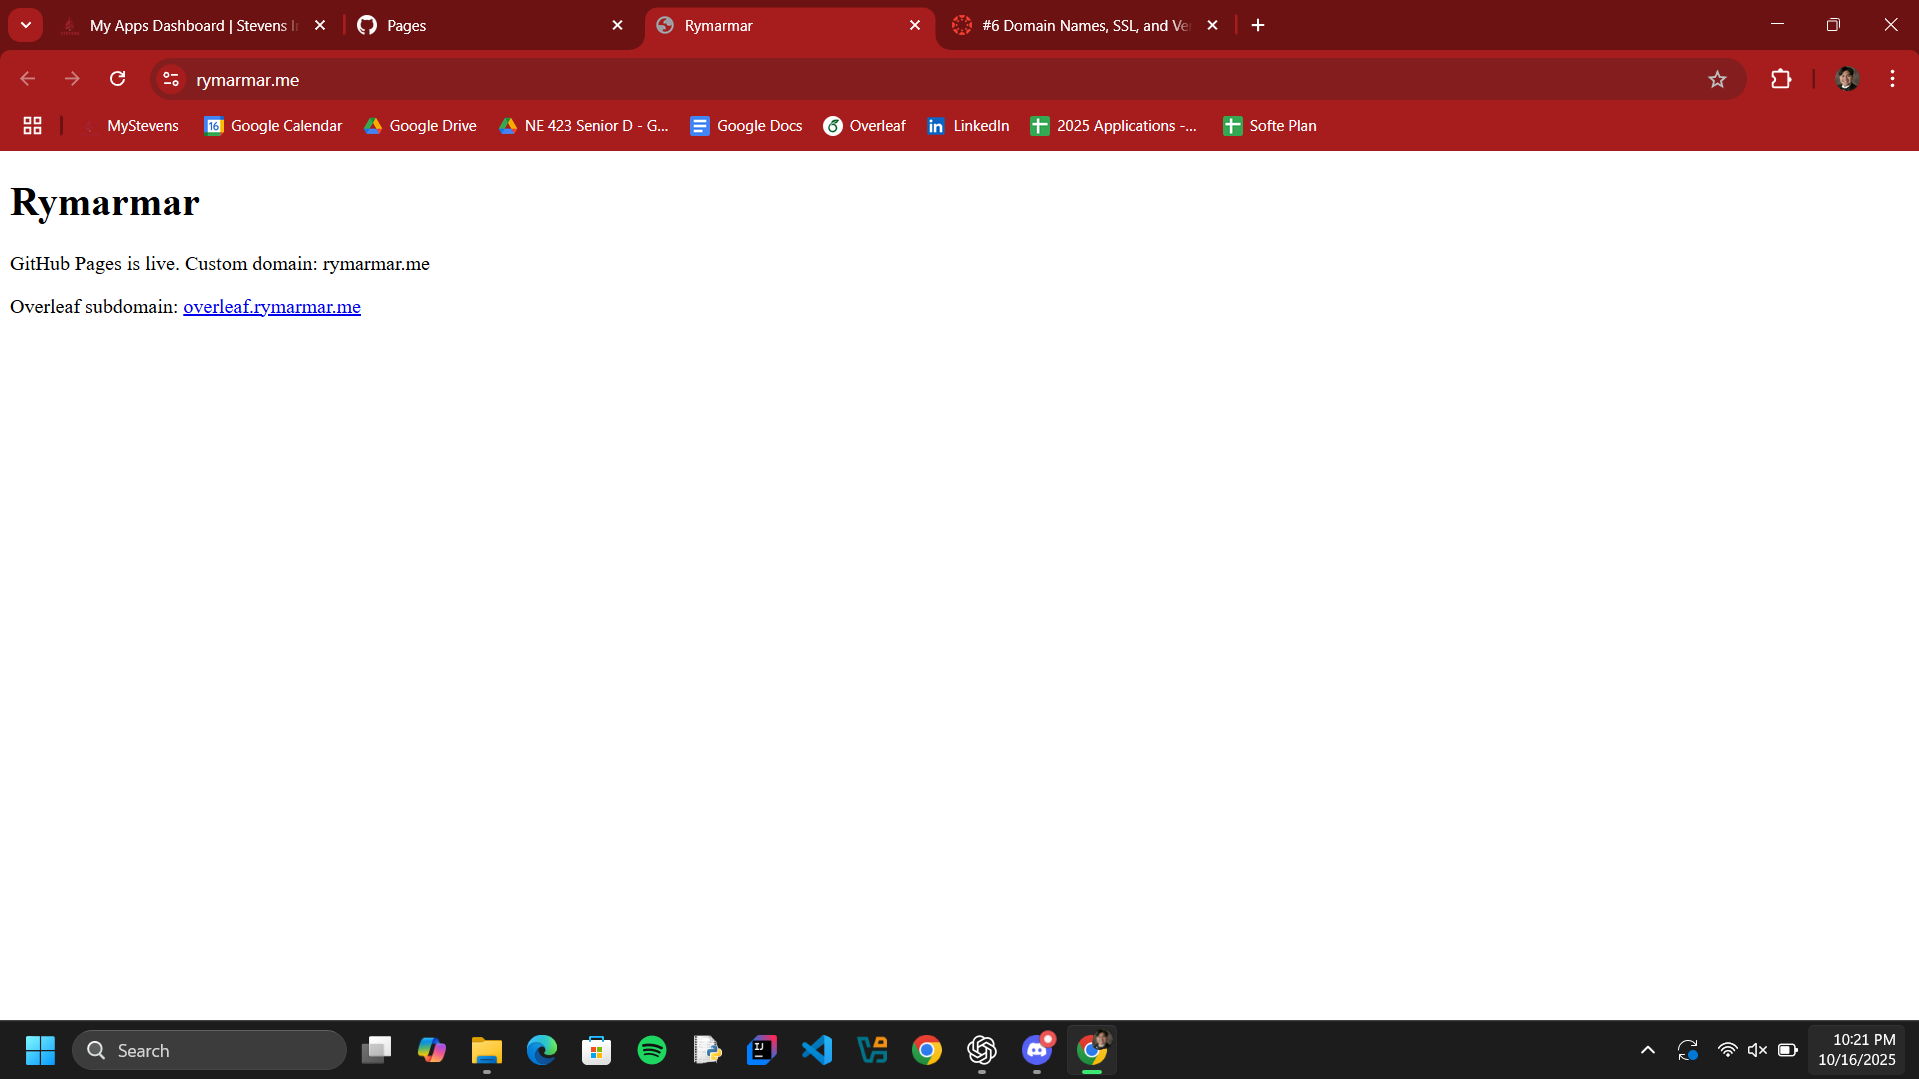
\includegraphics[width=\textwidth]{png/DomainNames/website.png}
    \caption{Deployed GitHub Pages site confirming build and domain resolution for \texttt{rymarmar.me}.}
\end{figure}

%----------------------------------------------------
\section{Step 5: Overleaf Subdomain Redirect Verification}
A subdomain \texttt{overleaf.rymarmar.me} was created in Namecheap and configured to redirect to our GitHub Pages site.  
This verifies that DNS records for the Overleaf subdomain resolve correctly.

\begin{figure}[h!]
    \centering
    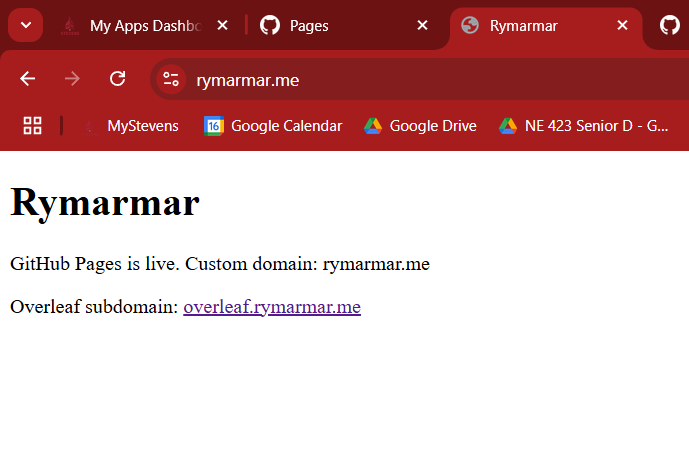
\includegraphics[width=\textwidth]{png/DomainNames/overleaf_redirect.png}
    \caption{The subdomain \texttt{overleaf.rymarmar.me} redirecting to the main site \texttt{rymarmar.me}.}
\end{figure}

%----------------------------------------------------
\section{Step 6: Overleaf–GitHub Sync (In Progress)}
Overleaf’s paid Git integration feature is unavailable for free users, so synchronization is currently being replicated manually using Git commands.  
The workflow allows us to update Overleaf projects locally and push them to GitHub for version tracking.

\begin{minted}{bash}
git clone https://github.com/Rymarmar/Overleaf.Rymarmar.me.git
cd Overleaf.Rymarmar.me
latexmk -pdf main.tex
\end{minted}

This process is being tested in parallel with the DigitalOcean instance to confirm compatibility between both platforms.

%----------------------------------------------------
\section{Step 7: Version Control and Hash Key (In Progress)}
To map each document version to a Git commit, versioning will be added to the LaTeX title once the sync process is finalized:

\begin{minted}{latex}
\title{SSW 590 - Domain Names, SSL, and Versioning (v1.0 - Commit 6fdbbf1)}
\end{minted}

This ensures full traceability between the Overleaf PDF and the GitHub repository version.

%----------------------------------------------------
\section{Conclusion and Deliverable Checklist}
This assignment demonstrates the end-to-end setup of a secured domain with SSL, integration with GitHub Pages, and configuration for an Overleaf instance hosted on DigitalOcean.  
Minor remaining work includes automating Overleaf <-> GitHub syncing and embedding commit hashes in titles for traceability.

\begin{itemize}
    \item[1.] \textbf{Domain Name:} Registered \texttt{rymarmar.me} via GitHub Student Pack – \checkmark
    \item[2.] \textbf{SSL Configuration:} HTTPS enforced via GitHub Pages / Let’s Encrypt – \checkmark
    \item[3.] \textbf{Overleaf Container Setup:} Hosted on DigitalOcean droplet – \checkmark
    \item[4.] \textbf{GitHub Pages Integration:} Site deployed and DNS verified – \checkmark
    \item[5.] \textbf{Overleaf Subdomain Redirect:} Verified redirect to GitHub Pages – \checkmark
    \item[6.] \textbf{Overleaf <-> GitHub Sync:} Manual workflow setup – \textit{In Progress}
    \item[7.] \textbf{Version/Hash in Title:} Format added, implementation pending – \textit{In Progress}
\end{itemize}

\chapter[GitHub Actions]{GitHub Actions \\\small{\textit{-- Charles, Justin, Benedict, Jacky}}}
\label{Chapter::GitHub Actions}
\index{Chapter!GitHub Actions}

\section{GitHub Actions Configuration}

\begin{enumerate}
    \item Using the Overleaf instance and GitHub repository we created in our  \nameref{Chapter::Domain Names} chapter 
    \item Create a new folder in the project named .github/workflows
    \item In that folder, create a .yml file which will contain the actions we want to use
    \item Push this file to the repo 
    \item Make changes to the Overleaf document and push them to the repository
    \item Check build status for successful compilation
\end{enumerate}
\\
\textbf{Our yml file}
\begin{minted}{Bash}
name: Compile LaTeX Documents

permissions:
  contents: write  # This allows the action to push changes back

on:
  push:
    branches: [ main, master ]
  pull_request:
    branches: [ main, master ]
  workflow_dispatch:

jobs:
  build:
    runs-on: ubuntu-latest
    
    steps:
    - name: Checkout repository
      uses: actions/checkout@v4
      with:
        fetch-depth: 0  # Get full history for version numbers
    
    - name: Get commit info
      id: commit
      run: |
        SHORT_HASH=$(git rev-parse --short HEAD)
        echo "short_hash=$(git rev-parse --short HEAD)" >> $GITHUB_OUTPUT
        echo "count=$(git rev-list --count HEAD)" >> $GITHUB_OUTPUT
    
    - name: Create builds directory
      run: mkdir -p builds

    - name: Update prologue.tex with commit hash
      run: |
        sed -i "s/GITHASHHERE/${{ steps.commit.outputs.short_hash }}/g" 2025F_SSW590_11/prologue.tex
        echo "Updated prologue.tex with commit hash: ${{ steps.commit.outputs.short_hash }}"

    - name: Compile LaTeX document
      uses: xu-cheng/latex-action@v3
      with:
        root_file: itManual.tex
        working_directory: 2025F_SSW590_11
        args: -pdf -interaction=nonstopmode -file-line-error -f
      continue-on-error: true
    
    - name: Create build info
      run: |
        echo "Build Information" > builds/BUILD_INFO.txt
        echo "================" >> builds/BUILD_INFO.txt
        echo "Commit: ${{ steps.commit.outputs.short_hash }}" >> builds/BUILD_INFO.txt
        echo "Build Number: ${{ steps.commit.outputs.count }}" >> builds/BUILD_INFO.txt
        echo "Date: $(date)" >> builds/BUILD_INFO.txt
        echo "Branch: ${{ github.ref_name }}" >> builds/BUILD_INFO.txt
    
    - name: Move PDFs to builds directory
      run: |
        # Define the source directory
        LATEX_DIR=2025F_SSW590_11
        
        # Check for the file in the correct subdirectory
        if [ -f $LATEX_DIR/itManual.pdf ]; then
          
          # Copy from the correct directory to the builds/ directory in the root
          cp $LATEX_DIR/itManual.pdf builds/itManual-${{ steps.commit.outputs.short_hash }}.pdf
          cp $LATEX_DIR/itManual.pdf builds/itManual-latest.pdf
          
          # Create a zip with the PDF and build info (CD to builds first)
          cd builds
          zip itManual-${{ steps.commit.outputs.short_hash }}.zip \
              itManual-${{ steps.commit.outputs.short_hash }}.pdf \
              BUILD_INFO.txt
          cd ..
          
        else
          echo "Error: PDF was not generated in $LATEX_DIR"
          exit 1
        fi 
    
    - name: Commit PDFs to repository
      run: |
        git config --local user.email "github-actions[bot]@users.noreply.github.com"
        git config --local user.name "github-actions[bot]"
        git add builds/
        git diff --staged --quiet || git commit -m "�� Add compiled PDF for commit ${{ steps.commit.outputs.short_hash }}"
        git push
    
    - name: Upload PDF artifacts
      uses: actions/upload-artifact@v4
      with:
        name: compiled-pdfs-${{ steps.commit.outputs.short_hash }}
        path: |
          builds/*.pdf
          builds/*.zip
          builds/BUILD_INFO.txt
        retention-days: 90
\end{minted}
\appendix
\chapter{Appendix \\
\small{\textit{-- Author Name}}
\index{appendix} 
\index{Chapter!Appendix}
\label{Chapter::Appendix}}


% makeglossaries dsnManual -- from command prompt.
\clearpage
%\printglossaries


\printnoidxglossaries

\bibliography{bibfile}
%\bibliographystyle{unsrt}
\bibliographystyle{IEEEtran}

\printindex
%\input{dsnManual.idx}
\end{document}
